\documentclass[final, 12pt, oneside]{class_diss}

\usepackage{eurosym}
\usepackage{algpseudocode}
\usepackage{amsmath}
\usepackage{amssymb}
\usepackage{amsthm}
\usepackage{amsxtra}
\usepackage[spanish, es-tabla]{babel}
\usepackage[usenames]{color}
\usepackage{graphicx}
\usepackage[utf8]{inputenc}
\usepackage{latexsym}
\usepackage[sort&compress]{natbib}
\usepackage{siunitx}
\usepackage{svg}
\usepackage[spanish]{translator}
\usepackage{pgfgantt}
\usepackage[hyphens]{url}
\usepackage[pdftex, plainpages=false, pdfpagelabels]{hyperref}
\usepackage{algorithm}
\usepackage[T1]{fontenc}
\usepackage[acronym, nonumberlist, numberedsection=nolabel]{glossaries}
\usepackage{hypernat}

\topmargin = -0.56in
\textheight = 8.60in
\textwidth = 6.46in
\oddsidemargin = 0.02in

\definecolor{Pink}{rgb}{1.0, 0.5, 0.5}
\definecolor{Maroon}{rgb}{0.8, 0.0, 0.0}

\hypersetup{
  linktocpage=true,
  colorlinks=true,
  citecolor=blue,
  urlcolor=red,
  linkcolor=Maroon,
  citebordercolor={1 0 0},
  urlbordercolor={1 0 0},
  linkbordercolor={0.7 0.8 0.8},
  breaklinks=true,
}

\bibpunct{}{}{,}{s}{}{}

\newacronym[longplural=servicios de regulación terciaria]{afrr}{aFRR}{servicio de regulación terciaria}

\newacronym[longplural=direcciones comunes de unidad de datos del servicio de aplicación]{asdu}{ASDU}{dirección común de unidad de datos del servicio de aplicación}

\newacronym[longplural=sistemas de almacenamiento de energía en baterías]{bess}{BESS}{sistema de almacenamiento de energía en baterías}

\newacronym[longplural=sistemas de control de baterías]{bms}{BMS}{sistema de control de baterías}

\newacronym[longplural=Boletines Oficiales del Estado]{boe}{BOE}{Boletín Oficial del Estado}

\newacronym[longplural=costes capitales]{capex}{CAPEX}{coste capital}

\newacronym[longplural=Comisiones Nacionales de los Mercados y la Competencia]{cnmc}{CNMC}{Comisión Nacional de los Mercados y la Competencia}

\newacronym[longplural=almacenes de datos]{dw}{DW}{almacén de datos}

\newacronym[longplural=reservas para la contención de frecuencia]{fcr}{FCR}{reserva para la contención de frecuencia}

\newacronym[longplural=interrogaciones generales]{gi}{GI}{interrogación general}

\newacronym[longplural=sistemas de control industrial]{ics}{ICS}{sistema de control industrial}

\newacronym[longplural=zonas industriales desmilitarizadas]{idmz}{IDMZ}{zona industrial desmilitarizada}

\newacronym[longplural=internets de las cosas industrial]{iiot}{IIoT}{internet de las cosas industrial}

\newacronym[longplural=direcciones de objeto de información]{ioa}{IOA}{dirección de objeto de información}

\newacronym[longplural=internets de las cosas]{iot}{IoT}{internet de las cosas}

\newacronym[longplural=tecnologías de la información]{it}{IT}{tecnología de la información}

\newacronym[longplural=indicadores de desempeño]{kpi}{KPI}{indicador de desempeño}

\newacronym[longplural=programaciónes lineales]{lp}{LP}{programación lineal}

\newacronym[longplural=programas diarios básicos de casación marginal]{marginalpdbc}{MARGINALPDBC}{programa diarios básico de casación marginal}

\newacronym[longplural=programas intradiarios básicos de casación incremental marginal]{marginalpibci}{MARGINALPIBCI}{programa diarios básico de casación incremental marginal}

\newacronym[longplural=servicios de regulación secundaria]{mfrr}{mFRR}{servicio de regulación secundaria}

\newacronym[longplural=mercados diarios]{md}{MD}{mercado diario}

\newacronym[longplural=mercados intradiarios]{mi}{MI}{mercado intradiario}

\newacronym[longplural=mercados intradiarios continuos]{mic}{MIC}{mercado intradiario continuo}

\newacronym[longplural=programaciónes lineales de enteros mixtos]{milp}{MILP}{programación lineal de enteros mixtos}

\newacronym[longplural=operadores del mercado]{mo}{MO}{operador del mercado}

\newacronym[longplural=unidades de tiempo de mercado]{mtu}{MTU}{unidad de tiempo de mercado}

\newacronym[longplural=Operadores del Mercado Ibérico de Energía]{omie}{OMIE}{Operador del Mercado Ibérico de Energía}

\newacronym[longplural=costes de operación]{opex}{OPEX}{coste de operación}

\newacronym[longplural=tecnologías operativas]{ot}{OT}{tecnología operativa}

\newacronym[longplural=programas diarios básicos finales]{pdbf}{PDBF}{programa diario básico final}

\newacronym[longplural=programas intradiarios básicos de casación acumulados]{pibca}{PIBCA}{programa intradiario básicos de casación acumulado}

\newacronym[longplural=arquitecturas de referencia empresarial de Purdue]{pera}{PERA}{arquitectura de referencia empresarial de Purdue}

\newacronym[longplural=sistemas de conversión de energía]{pcs}{PCS}{sistema de conversión de energía}

\newacronym[longplural=puntos frontera]{pf}{PF}{punto frontera}

\newacronym[longplural=sistemas de información de planta]{pis}{PIS}{sistema de información de planta}

\newacronym[longplural=Redes Eléctricas Españolas]{ree}{REE}{Red Eléctrica Española}

\newacronym[longplural=unidades terminales remotas]{rtu}{RTU}{unidad terminal remota}

\newacronym[longplural=sistemas de comunicación\, ejecución y control de la interrumpibilidad]{sceci}{SCECI}{sistema de comunicación, ejecución y control de la interrumpibilidad}

\newacronym[longplural=estados de carga]{soc}{SoC}{estado de carga}

\newacronym[longplural=estados de salud]{soh}{SoH}{estado de salud}

\newacronym[longplural=operadores del sistema de transimisón]{tso}{TSO}{operador del sistema de transmisión}

\newacronym[longplural=unidades físicas]{ufi}{UFI}{unidad física}

\newacronym[longplural=unidades de oferta]{uof}{UOF}{unidad de oferta}

\newacronym[longplural=unidades de programación]{up}{UP}{unidad de programación}

\makeglossaries

\begin{document}

\section*{Todo}
\begin{enumerate}
  \item Acrónimos MD MI MIC LP MILP
  \item Imágenes y tablas optional caption \texttt{\textbackslash caption[]\{\}} para que no salgan las citas en el indice de figuras y tablas
  \item Redactar capítulo estado de la cuestión (1 día)
  \item ¿Anexo de símbolos? (1 día)
  \item Completar figuras (2 días)
\end{enumerate}

\setcounter{page}{-1}

\newpage

\thispagestyle{empty}

\begin{center}

  \vspace{1cm}

  {\large OPTIBAT\@: OPTIMIZACIÓN DE BATERÍAS EN EL MERCADO ELÉCTRICO}\\

  \vspace{0.5cm}

  \vspace{0.5cm}

  {\large JOSU GOMEZ ARANA}\\

  \vspace{0.5cm}

  MÁSTER EN INTERNET DE LAS COSAS\@. FACULTAD DE INFORMÁTICA\\
  UNIVERSIDAD COMPLUTENSE DE MADRID\\

  \vspace{0.65cm}

  \rule{2in}{0.5pt}\\

  \vspace{0.85cm}

  
\includegraphics[height=2.5in]{figures/escudo.jpg}

  \vspace{0.5cm}

  Trabajo Fin Máster en Internet de las Cosas

  \vspace{0.5cm}

  15 de septiembre de 2025\\

  \vspace{1cm}

\end{center}

{
  \raggedleft
  Director/es:\\
  \vspace{1cm}
  Francisco Daniel Igual Peña\\
  Luis Piñuel Moreno\\
}

\pdfbookmark[0]{Portada}{PDFPortadaPage}

\newpage

\thispagestyle{empty}

\begin{center}

  {\bf \Huge Autorización de difusión}

  \vspace{1cm}

  \large Josu Gomez Arana

  \vspace{0.5cm}

  5 de septiembre de 2025

  \vspace{0.5cm}

\end{center}

El/la arriba firmante, matriculado/a en el Máster en Investigación en Informática de la Facultad de Informática, autoriza a la Universidad Complutense de Madrid (UCM) a difundir y utilizar con fines académicos, no comerciales y mencionando expresamente a su autor el presente Trabajo Fin de Máster: “OPTIBAT\@: OPTIMIZACIÓN DE BATERÍAS EN EL MERCADO ELÉCTRICO”, realizado durante el curso académico 2024--2025 bajo la dirección de Francisco Daniel Igual Peña y Luis Piñuel Moreno en el Departamento de Informática, y a la Biblioteca de la UCM a depositarlo en el Archivo Institucional E-Prints Complutense con el objeto de incrementar la difusión, uso e impacto del trabajo en Internet y garantizar su preservación y acceso a largo plazo.

\pdfbookmark[0]{Autorización}{PDFAutorizacionPage}

\newpage

\thispagestyle{empty}

\begin{center}
  {\bf \huge Resumen en castellano}
\end{center}

\vspace{1cm}

En respuesta a la creciente adopción de los sistemas de almacenamiento de energía en baterías y la ausencia de soluciones actualmente en producción principalmente centradas en configuraciones topológicas híbridas, se define el diseño, desarrollo, despliegue y validación de \textsc{Optibat}, un sistema integral para la automatización del arbitraje en el mercado eléctrico. El sistema busca maximizar la rentabilidad económica comprando y vendiendo energía en los mercados spot mediante el control del ciclado de las baterías. Para ello, se integran datos operacionales en tiempo real de los activos energéticos con la información del entorno del operador del mercado y operador del sistema, empleando un modelo de programación lineal de enteros mixtos para determinar la estrategia óptima de carga y descarga e interactuando directamente con los agentes de mercado y operadores de telecontrol. Desplegado con éxito en múltiples instalaciones a gran escala, \textsc{Optibat} gestiona docenas de megavatios hora diarios y genera millones de euros de ingresos anuales previstos. Los resultados demuestran que las topologías híbridas son significativamente más rentables que las aisladas, destacando el modelo por su capacidad para aumentar el aprovechamiento de la generación energética. De esta forma, el proyecto aporta una solución robusta y escalable que valida el caso de negocio de las baterías, permitiendo su integración eficaz como activos óptimos y fiables en el mercado eléctrico.

\vspace{1cm}

\begin{center}
  {\bf \large Palabras clave}
\end{center}

\vspace{0.5cm}

Internet de las cosas industrial, sistema de almacenamiento de energía en baterías, mercado eléctrico, optimización energética, telecontrol

\pdfbookmark[0]{Resumen}{PDFResumenPage}

\vfill

\newpage
\pagenumbering{roman}
\setcounter{page}{1}

\phantomsection
\addcontentsline{toc}{chapter}{Índice}

\tableofcontents
\listoffigures
\listoftables

\newpage
\pagenumbering{arabic}
\setcounter{page}{1}

\cleardoublepage

\chapter{Introducción}
\label{makereference1}

\begin{quotation}

  El calor aprieta. Tratas de distraerte de las altas temperaturas y aliviar la pesadez del aire con tu programa favorito refrescante bebida en mano. En cambio, la nevera se mantiene inusualmente silenciosa, el ventilador permanece inmóvil y la televisión no parece despertar. Lentamente, la habitación se sume en la oscuridad.

  Un tiempo después, toda la estancia repentinamente se inunda nuevamente en la luz de las lámparas previamente impotentemente encendidas que vuelven a la vida, el apagón parece haber concluido. Comprendes que, acostumbrado a bastar con apretar el interruptor, rara vez reflexionas en el complejo entramado eléctrico detrás de algo tan simple que permanece oculto ante la mirada común.

\end{quotation}

El sistema energético por detrás de la totalidad de la generación, transporte y distribución de la electricidad se mantiene entendiblemente completamente transparente ante los ojos de los usuarios finales de dicha energía~\cite{garrues2009red}.

Por un lado, existe un entramado de redes de transporte eléctrico que combina múltiples tecnologías para asegurar su funcionamiento, teniendo que disponer de una elevada complejidad con el fin de integrar las diversas características del entorno cambiante de los activos energéticos.

Por otro, las partes interesadas realmente compran y venden la energía en masa en el llamado mercado de la electricidad, en el cual se determina finalmente su precio puntual. Esto da lugar a dinámicas de arbitraje con el objetivo de generar beneficio económico, al igual que sucede con cualquier otro activo financiero.

En la actualidad, existen multitud de soluciones energéticas con las que aprovisionar la red de energía y arbitrar en el mercado, como la generación fotovoltaica, eólica, hidráulica o ciclo combinado. Aunque todas ellas juegan un papel más que fundamental en el sistema energético~\cite{turkenburg2000renewable}, una de ellas destaca por encima del resto, especialmente por su creciente popularidad. Se trata de los \glspl{bess}, ilustrados en la figura~\ref{fig:instalacion-bess}.

\begin{figure}
  \centering
  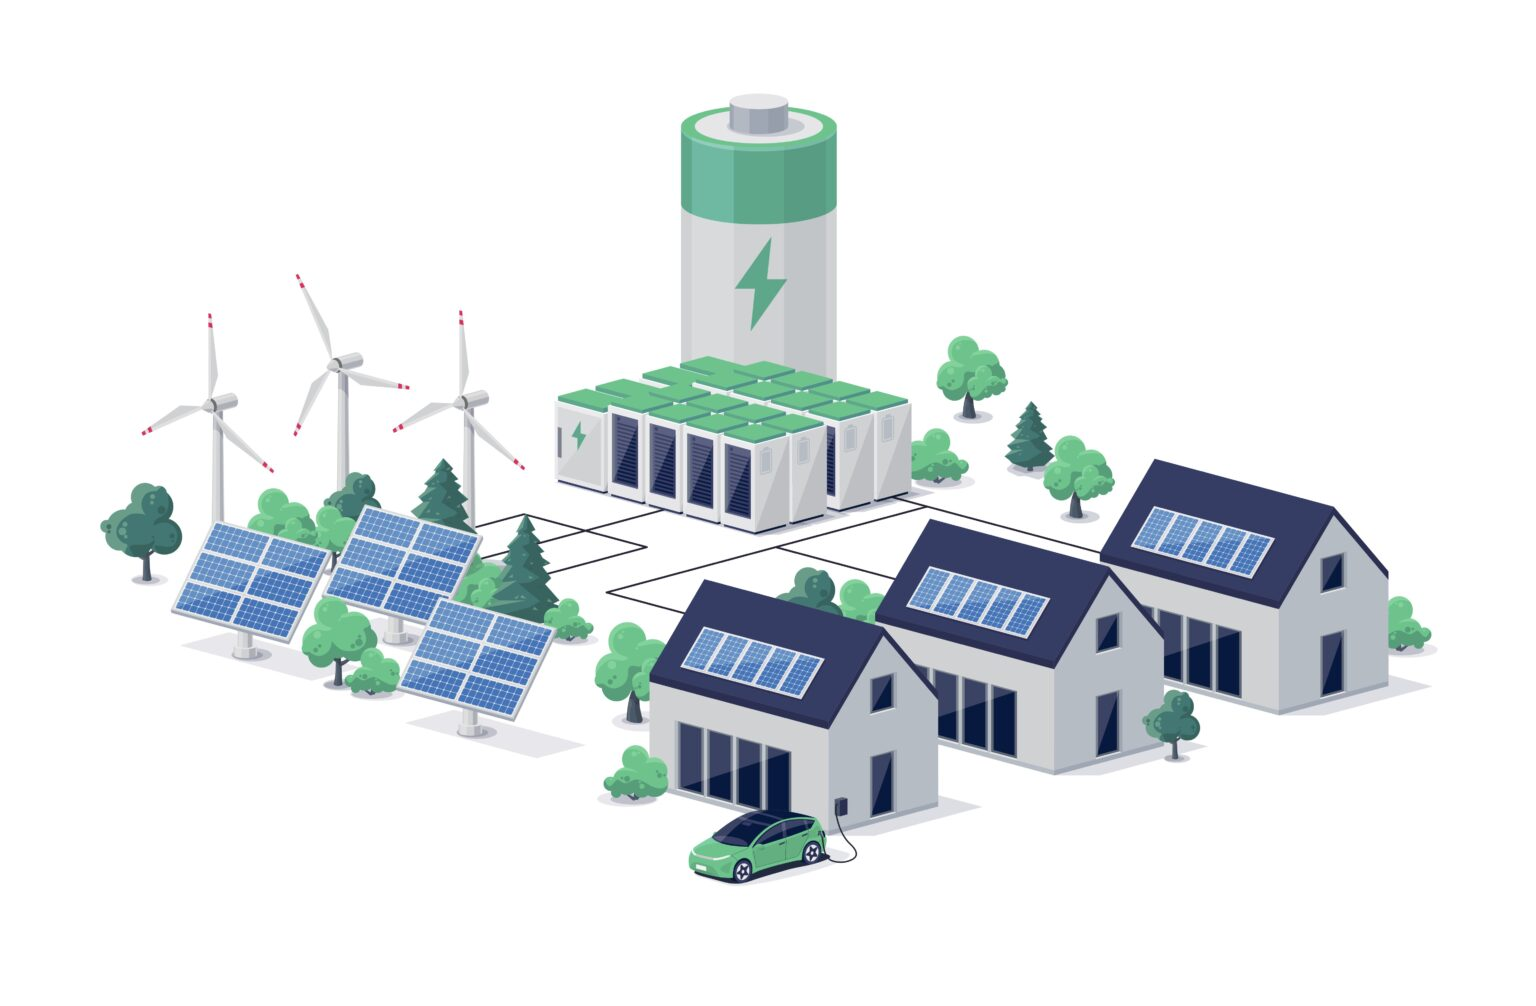
\includegraphics[width=0.5\linewidth]{figures/instalacion-bess.jpg}
  \caption{Ilustración de la disposición una instalación híbrida de generación y almacenamiento\cite{deutz2023what}}
  \label{fig:instalacion-bess}
\end{figure}

Precisamente, los \glspl{bess} son una comparativamente novedosa tecnología energética de almacenamiento que permiten, como su propio nombre indica, almacenar electricidad para su uso posterior. Esto facilita enormemente la gestión de la demanda y, crucialmente, mejora la estabilidad y eficiencia de la infraestructura eléctrica, pudiendo regularla activamente gracias a la rápida capacidad de conmutación de las baterías. De esta forma, son una de las tecnologías energéticas más idóneas para evitar posibles desajustes en la red~\cite{xu2014bess}.

Aún y todo, no sirve con disponer únicamente de las baterías, sino que, más que nada, es justamente imprescindible controlar la carga y descarga de estos dispositivos cuidadosamente para prolongar su vida útil y asegurar el correcto funcionamiento de los mismos. Como las baterías cuentan con un \gls{capex} inicialmente considerable, pero un \gls{opex} mínimo~\cite{larsson2018cost}, lo que se busca es su rentabilidad mediante el beneficio generado a través del arbitraje de la energía almacenada en el mercado eléctrico.

Es entonces cuando surge la necesidad de la creación de un sistema de optimización de baterías en el mercado eléctrico basado en el \gls{iiot}, el cual gestione tanto la infraestructura operacional, el entorno de mercado, la modelización estructural y el comando y control, continuamente ciclando la batería incansablemente en busca de los mejores márgenes.

De hecho, así es como nace Optibat, el sistema de optimización de baterías en el mercado eléctrico de desarrollo propio desplegado satisfactoriamente en múltiples instalaciones energéticas a lo largo del país, que mueve docenas de megavatios hora al día y genera millones de euros de ingresos previstos al año.

Con esto, se detallan las decisiones de diseño relacionadas con la integración del sistema y los componentes de la arquitectura ya existentes (es decir, sapectos fundamentales de la operación que la entidad energética dueña de los activos energéticos tenía disponibles con anterioridad), el desarrollo con respecto a la creación de todos los elementos propios a tener en cuenta, la validación para asegurar la seguridad y correcto funcionamiento, el despliegue en relación a la puesta en marcha en instalaciones a gran escala y la experimentación comparativa en busca del mejor modo de operación.

De esta forma, el sistema se divide en los apartados anteriormente mencionados. La infraestructura operacional, explicada en el capítulo~\ref{makereference3}, gestiona la capa de interacción de menor nivel disponible. El entorno de mercado, especificado en el capítulo~\ref{makereference4}, determina la información extraída de las instituciones regulatorias con las que se trabaja. La modelización estructural, puntualizada en el capítulo~\ref{makereference5}, habla de la lógica de negocio de las decisiones a tomar. El comando y control, precisado en el apartado~\ref{makereference6}, explica el flujo de vuelta a los activos físicos y la interacción de los agentes de mercado y operadores de telecontrol con el sistema. Finalmente, se describe la experimentación realizada en el capítulo~\ref{makereference7}.

\section{Objetivos}
\label{makereference1.1}

El objetivo principal es el diseño, desarrollo, validación y despliegue (excluyendo la experimentación) de un sistema de arbitraje de baterías en el mercado eléctrico, garantizando su integración con la infraestructura establecida y su habilitación para operar en el mercado eléctrico. Cabe destacar que, dado que la tecnología de almacenamiento de energía en baterías apenas se encuentra aún en su infancia, no existe una solución fácilmente integrable o de sencilla implementación sobre la infraestructura energética existente, aunque existan esfuerzos externos para mejorar la situación. Por ello, lo que primeramente se busca es establecer dicha base.

A su vez, se definen varios objetivos secundarios complementarios al objetivo principal anterior.

\begin{description}

  \item[Maximizar la rentabilidad] Más allá de hacer funcionar el sistema, obtener la mayor rentabilidad entre la energía comprada y vendida es lo primordial. El sistema debe ser capaz de analizar las previsiones de precios del mercado eléctrico para programar de forma óptima los ciclos de carga y descarga, asegurando la compra de energía en los periodos de menor coste y su venta en los de mayor precio, además de tener en cuanta factores externos al mercado y rentabilizar los \glspl{capex} y \gls{opex}. Lo más importante es diferenciar el beneficio neto en euros y la rentabilidad en euros por megavatio hora como determina la \gls{cnmc} en el \gls{boe}~\cite{cnmc2025resolucion}, ya que esta última es la métrica verdaderamente usada para asegurar que se asigna el valor correcto a las unidades de energía usada.

  \item[Minimizar el desgaste de las baterías] Se busca gestionar la operación del activo, principalmente la profundidad de descarga y el número de ciclos, de manera que se prolongue su vida útil y se minimice el desgaste físico del \gls{soc}. Se pretende encontrar el equilibrio entre la rentabilidad a corto plazo y la sostenibilidad de la inversión a largo plazo (ganar mucho dinero cuanto antes pero gastar la batería contra no ofertar tan agresivamente y estabilizar el ciclado pudiendo aprovechar mejores oportunidades futuras). La métrica usada para medir el desgaste se trata del número de ciclos de carga completos que, a diferencia del \gls{soh}, permite estimar la evolución del desgaste más fácilmente.

  \item[Cumplir con los requisitos regulatorios] Es altamente aconsejable que todas las operaciones de carga y descarga propuestas por el sistema se adhieran estrictamente a los requisitos técnicos y normativos impuestos por tanto el \gls{mo} como el \gls{tso}~\cite{crespo2004resolucion}. Esto incluye el respeto de los límites de potencia estructurales marcados por ley, los límites técnicos causados por indisponibilidades, etc. El cumplimiento se mide a través de la magnitud de la desviación final por periodo de mercado en megavatios hora, es decir, la cantidad de energía que el sistema a pactado pero no ha sido capaz de cubrir.

  \item[Garantizar la seguridad de la operación] Se deben implementar múltiples niveles de validación para prevenir cualquier operación que pueda comprometer la integridad física del \gls{bess} o de la información misma. Aunque el control de bajo nivel es responsabilidad del \gls{bms} nativo de la batería, el sistema de optimización tiene la obligación de operar siempre dentro de un rango seguro predefinido. Además, la información tiene que fluir adecuándose correctamente a la \gls{pera}~\cite{williams1994purdue} de ciberseguridad en el entrono industrial. La seguridad de la operación se mide de forma empírica teniendo en cuenta el número de alarmas causadas por los sistemas de almacenamiento y alertas de ciberseguridad.

  \item[Generalizar el diseño] El diseño de una arquitectura modular y configurable resulta clave para permitir la adaptación del sistema a diferentes instalaciones con capacidades de almacenamiento y configuraciones variadas. El objetivo es crear una solución escalable, no específica s una única instalación, facilitando su despliegue en futuras instalaciones con un esfuerzo de integración mínimo. La modularidad se analiza mediante el número íntegro de instalaciones soportadas por el sistema en el momento de su despliegue.

  \item[Facilitar la monitorización del sistema] Una interfaz de comando y control, que permita a los operadores de telecontrol y agentes de mercado supervisar el estado del sistema en tiempo real, ayuda a aumentar la confianza en el mismo. Esta interfaz debe proporcionar una visualización clara de las operaciones planificadas y ejecutadas y los resultados económicos obtenidos, garantizando la transparencia y la trazabilidad de las decisiones del sistema. Crucialmente, los agentes de mercado deben ser capaces de sobrescribir el comportamiento automático del sistema con indicaciones manuales ante situaciones de mercado no tenidas en cuenta, o periodos de prueba en el caso de los operadores de telecontrol.

  \item[Responder ante fallos] Se dota al sistema de mecanismos de detección y gestión de fallos, tanto internos como, principalmente, externos, para asegurar su robustez y alta disponibilidad. Esto incluye la capacidad de gestionar interrupciones en la operación de la disponibilidad de los activos físicos o la pérdida o información incompleta de los datos de mercado, debiendo tener en cuenta dichas situaciones explícitamente de tal forma que el funcionamiento del sistema, más allá de dicha particularidad, no se vea afectado. Medido programáticamente mediante el número indisponibilidades no causadas por factores externos, sino por el sistema.

  \item[Analizar la viabilidad económica] Utilizando los datos operativos y los resultados del sistema se busca realizar un análisis de viabilidad económica posterior. El objetivo es validar el caso de negocio, cuantificar con precisión la rentabilidad obtenida teniendo en cuenta los \glspl{capex} y \glspl{opex} y modelar el rendimiento financiero del activo bajo diferentes escenarios de mercado. Este análisis sirve para refinar las estrategias de operación y guiar futuras inversiones en los sistemas de almacenamiento de energía en baterías, intentando validar así la aparente predisposición al beneficio de las baterías como activo energético. Se mide en euros megavatio hora relativos. Se trata de un análisis posterior ya que se considera con anterioridad la tesis del beneficio de rentabilidad de los \glspl{bess}.

\end{description}

\section{Alcance}
\label{makereference1.2}

El proyecto se centra exclusivamente en el desarrollo de un sistema de optimización de baterías en el mercado eléctrico integral, de extremo a extremo. Se compone de la infraestructura operacional con la que interactuar con los elementos físicos que forman parte del sistema, la adquisición de la información del entorno de mercado a través de las instituciones regulatorias correspondientes, la modelización estructural de la situación del ciclado de las baterías y de la instalación al completo para la resolución de la optimalidad, y el comando y control para transmitir los resultados de vuelta a la batería y mercado e informar a los agentes de mercado que supervisan los movimientos realizados por el sistema.

En cambio, el alcance no incluye el control físico del nivel eléctrico de las instalaciones, realizado por el \gls{bms} que viene incluido en los \glspl{bess} industriales y es implantado a gran escala por el integrador del sistema, como lo es Ingeteam~\cite{ingeteam2022ingeteam}, debido a obvias consideraciones de seguridad y de acceso físico restringido.

Tampoco se realiza el despliegue en sí del \gls{pis} central, ya que otras tecnologías energéticas hacen uso del mismo más allá de las baterías. Esto no quita que, aunque el sistema de control de planta ya exista de antes, el sistema desarrollado realize la integración de los activos energéticos físicos mismos con el \gls{pis} mismo mediante su extensión, a única excepción de su despliegue.

Finalmente, el proyecto debe considerar procesos externos del entorno en el que es desplegado, por lo que no hay otra opción que depender de la capa de indirección del almacenamiento de la información del entorno de mercado (el \gls{dw}), del desglose de las posiciones negociadas previamente consultadas en servicios internos, y de la última etapa de la realización de las ofertas de mercado, la cual debe, por consideraciones legales, realizarse por la parte confiable de la entidad energética dueña de los activos energéticos.

Con esto, la implementación de los apartados no confidenciales se encuentra a disposición bajo solicitud.

% TODO
\section{Plan de trabajo}
\label{makereference1.3}

El plan de trabajo consta de la distribución en tareas del desarrollo del proyecto en su conjunto. Se constituye de la división de los apartados en concordancia con los objetivos, desde el inicio hasta el final del proyecto integrado, y de la explicación de estos.

\begin{figure}[h]
  \centering
  \resizebox{\textwidth}{!}{
    \begin{ganttchart}[x unit=1mm, time slot format=isodate, time slot unit=day]{2025-02-10}{2025-09-15}
      \gantttitlecalendar{month=shortname} \\
      \ganttgroup[name=análisis]{Análisis preliminar}{2025-02-10}{2025-03-09} \\
      \ganttgroup[name=desarrollo]{Desarrollo}{2025-03-10}{2025-07-31} \\
      \ganttgroup[name=experimentación]{Experimentación}{2025-07-01}{2025-08-04} \\
      \ganttgroup[name=redacción]{Redacción del informe}{2025-07-01}{2025-09-15} \\
      \ganttlink{análisis}{desarrollo}
      \ganttlink{desarrollo}{experimentación}
      \ganttlink{experimentación}{redacción}
    \end{ganttchart}
  }
  \caption{Diagrama Gantt del plan de trabajo}
  \label{fig:plan-trabajo}
\end{figure}

\begin{description}

  \item[Task 1] Lorem ipsum

  \item[Task 2] Lorem ipsum

  \item[Final Task] Lorem ipsum

\end{description}

\cleardoublepage

\chapter{Estado de la cuestión}
\label{makereference2}

% - estado inicial con la herramienta original que no funcionaba? DECIR QUE APENAS HABÍA NADA ANTES

Contextualizando el entorno, la transición hacia un sistema energético descarbonizado, impulsada por la creciente penetración de fuentes de energía renovable, como la solar fotovoltaica y la eólica, presenta desafíos significativos para la estabilidad y gestión de la red eléctrica~\cite{carrasco2023battery}. De esta forma, los \gls{bess} emergen como una tecnología clave para dotar de flexibilidad al sistema, solucionando el desacoplo entre la generación y el consumo de electricidad~\cite{gissey2018market}.

El mercado eléctrico, que opera usando un modelo marginalista para los mercados spot en donde el precio es determinado mediante el cruce de la oferta y demanda mostrado en la figura~\ref{fig:precio-casacion}, ofrece diversas oportunidades para los \glspl{bess}. Estas incluyen el arbitraje de energía en los mercados spot diario intradiarios y continuo, en los que se centra el sistema desarrollado, y la participación en los servicios de ajuste~\cite{gaspar2021optimisation}, \gls{afrr} y \gls{mfrr}, donde se arbitran disponibilidades. Por ello, la viabilidad económica depende intrínsecamente de la capacidad del sistema para formular y ejecutar estrategias de operación óptimas en un entorno de alta incertidumbre de precios y previsiones de generación~\cite{heredia2015economic}, llamándose incluso una ``tecnología clave''.

\begin{figure}
  \centering
  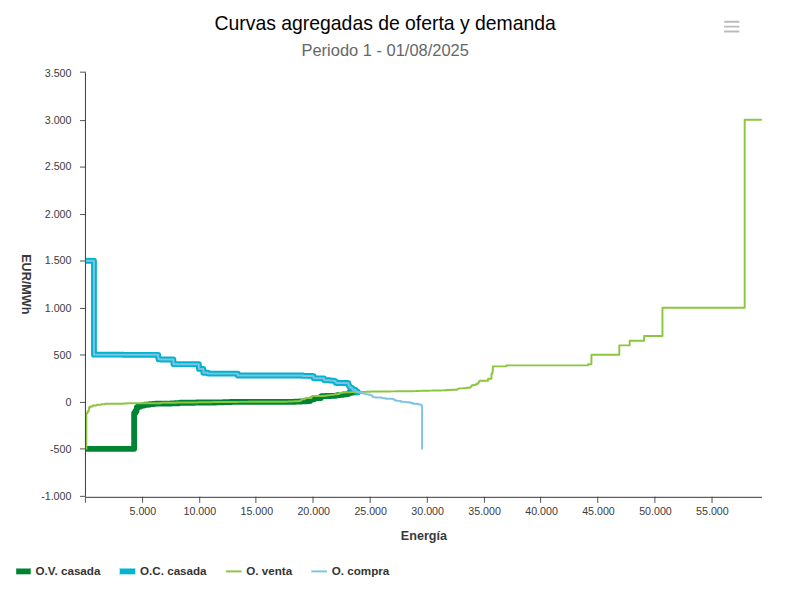
\includegraphics[width=0.5\linewidth]{figures/precio-casacion.png}
  \caption{Curva de casación real del inicio del mes de agosto del mercado eléctrico marginalista extraída de \gls{omie}, donde tan solo las ofertas de compra por encima y de venta por debajo del precio de casación son aceptadas.}
  \label{fig:precio-casacion}
\end{figure}

\section{Situación tecnológica}

La situación tecnológica de los optimizadores de \glspl{bess} varía significativamente entre los mercados eléctricos ibéricos, del resto de Europa y de Estados Unidos, debido a diferencias en el diseño de los mercados, los marcos regulatorios y los incentivos políticos.

\chapter{Infraestructura operacional}
\label{makereference3}

El desarrollo del sistema, visto desde una perspectiva \textit{bottom-up}, comienza con la capa de abstracción más baja, correspondiente con la infraestructura operacional.

Esta infraestructura, mayormente relacionada con el apartado físico del paradigma del \gls{iiot}, integra el hardware de campo con el software de análisis y constituye el pilar fundamental del sistema. Actúa como la conexión indispensable entre los dispositivos y sensores físicos reales, la lógica abstracta del modelo de optimización matemática y la comunicación de vuelta con los resultados obtenidos.

Como es entendible, el desarrollo ha hecho uso de la infraestructura operacional ya existente en cuanto a la red interna de las instalaciones a controlar. De cualquier otro modo, el despliegue real del sistema desarrollado no hubiera sido posible, ya que se necesitarían recursos a gran escala no comúnmente disponibles, pudiendo visualizar el activo energético principal en cuestión en la figura~\ref{fig:diagrama-bess}.

\begin{figure}
  \centering
  \includesvg[width=0.5\linewidth]{figures/diagrama-bess.svg}
  \caption[Diagrama de un sistema de almacenamiento de energía en baterías.]{Diagrama de un sistema de almacenamiento de energía en baterías~\cite{iberdrola2024bess}.}
  \label{fig:diagrama-bess}
\end{figure}

Por ello, la principal contribución del apartado de la infraestructura operacional se ve reflejada en la configuración, securización, despliegue y validación de la herramienta de conexión entre los activos físicos y del historiador del \gls{pis}, a través de los correspondientes protocolos de comunicación posteriormente descritos. Se busca la integración estandarizada con los componentes ya existentes, para el correcto funcionamiento de las instalaciones que alojan los \glspl{bess}, mientras se tiene en cuenta que los sistemas de almacenamiento apenas son una pequeña parte de la red al completo.

De esta forma, es posible obtener una visión más completa a través del análisis realizado en la sección~\ref{makereference3.1}, que define la arquitectura de la disposición de los activos energéticos y las múltiples restricciones operativas fundamentales tenidas en cuenta por el desarrollo. También, se examinan los componentes físicos que forman parte de la infraestructura al completo, detallados en la sección~\ref{makereference3.2}, que actúan como la fuente primaria de la obtención de datos. Además, se explora la comunicación que unifica estos componentes en la sección~\ref{makereference3.3},  facilitando un intercambio de datos estandarizado. Con esto, se describe la gestión de la información obtenida en la sección~\ref{makereference3.4}, detallando su rol en el almacenamiento, la gestión y la validación de los datos operativos. Por último, se explica como los datos de la infraestructura obtenidos son transformados y consumidos en la sección~\ref{makereference3.5}.

\section{Configuración topológica}
\label{makereference3.1}

Resulta que en los \glspl{bess}, la efectividad operativa y la rentabilidad, esta última sobre todo, no dependen exclusivamente de la tecnología intrínseca utilizada o de la optimalidad de su operación, sino que están condicionadas fundamentalmente por su configuración topológica.

Esta disposición es absolutamente necesaria para llegar a comprender el funcionamiento de la representación operacional de las plantas, ya que una de las principales motivaciones del desarrollo del sistema ha resultado ser la intención de aprovechar las ventajas de que brindan las topologías más avanzadas e integradas con el resto de activos, como lo es la topología híbrida aquí descrita. Posteriormente, en el apartado~\ref{makereference5} de modelización estructural se describe la implementación de la lógica topológica y en el apartado~\ref{makereference7} de resultados experimentales las diferencias en la operación de las topologías.

Así, la topología de una instalación energética se refiere a la arquitectura física de conexión de los activos energéticos con la red eléctrica y otros elementos de generación o consumo dentro de la instalación misma en todo su conjunto~\cite{parlikar2019topology}.

Esta define los flujos energéticos posibles y, por ello, impone las restricciones estructurales que el modelo de optimización debe considerar como premisas inviolables para garantizar la validez física y económica de las soluciones.

Precisamente, estos flujos energéticos son los que dictan los canales de importación y exportación de energía entre la red pública de alta tensión, controlada por el \gls{tso}, y la red interna de media tensión de la entidad energética, manejadas las instalaciones de almacenamiento mismas por el control del sistema desarrollado, a través del llamado \gls{pf}.

De igual manera, es necesario subrayar la relevancia de los flujos energéticos nuevamente, ya que todas y cada una de las operaciones en el mercado se realizan a través ellos, cada uno poseyendo una identificación correspondiente al flujo energético pertinente, como se muestra en la tabla~\ref{tab:unidades-fisicas}.

\begin{table}[ht]
  \centering
  \begin{tabular}{|l|l|l|l|}
    \hline
    UFI     & UP      & UOF     & Descripción         \\
    \hline
    BPLLANC & AFIBHFC & AFIBHFC & Batería Compra      \\
    BPLLANV & FBHIBHV & IBEVD22 & Batería Venta       \\
    PLLANO  & FBHIBHV & IBEVD22 & H.B. Puertollano II \\
    BURKIC  & AFIBHEC & AFIBHEC & Batería Compra      \\
    BURKIV  & EBHIBHV & IBEVD24 & Batería Venta       \\
    ELGURKI & EBHIBHV & IBEVD24 & P.E. Elgea-Urkilla  \\
    \hline
  \end{tabular}
  \caption[Unidades físicas, de programación y de oferta.]{Unidades físicas, de programación y de oferta de múltiples instalaciones.}
  \label{tab:unidades-fisicas}
\end{table}

Los flujos energéticos, o, mejor expresado, las interfaces correspondientes a los mismos, son conocidos como \gls{ufi}, mientras que la interfaz que oferta a mercado y engloba las \glspl{ufi} es llamada \gls{up} desde el punto de vista del \gls{tso} y \gls{uof} desde la perspectiva del \gls{mo}.

El sistema desarrollado, por tanto, hace uso de la configuración topológica ya existente, es decir, no se encarga de la implantación física de los activos energéticos o de la conexión de los mismos con la red física, ya que eso queda bien fuera del alcance del diseño. En cambio, sí que hace uso de los diferentes componentes mediante sus correspondientes canales.

De esta forma, en términos generales y en el ámbito del mercado eléctrico peninsular, como es el caso, las instalaciones que alojan baterías de escala industrial se pueden clasificar principalmente en dos grandes familias, la configuración aislada y la híbrida, basada la terminología en las definiciones oficiales del Estado~\cite{cnmc2024servicios}.

\subsection{Topología aislada}
\label{makereference3.1.1}

La configuración aislada o \textit{standalone} representa el arquetipo más directo de despliegue de un \gls{bess}~\cite{gallo2023stand}.

En esta topología, la batería es el único activo energético de la instalación y su principal propósito es interactuar con la red eléctrica pública de alta tensión, conectada a través del \gls{pf} a la red interna de media tensión, como se observa en la figura~\ref{fig:topologia-aislada}.

\begin{figure}
  \centering
  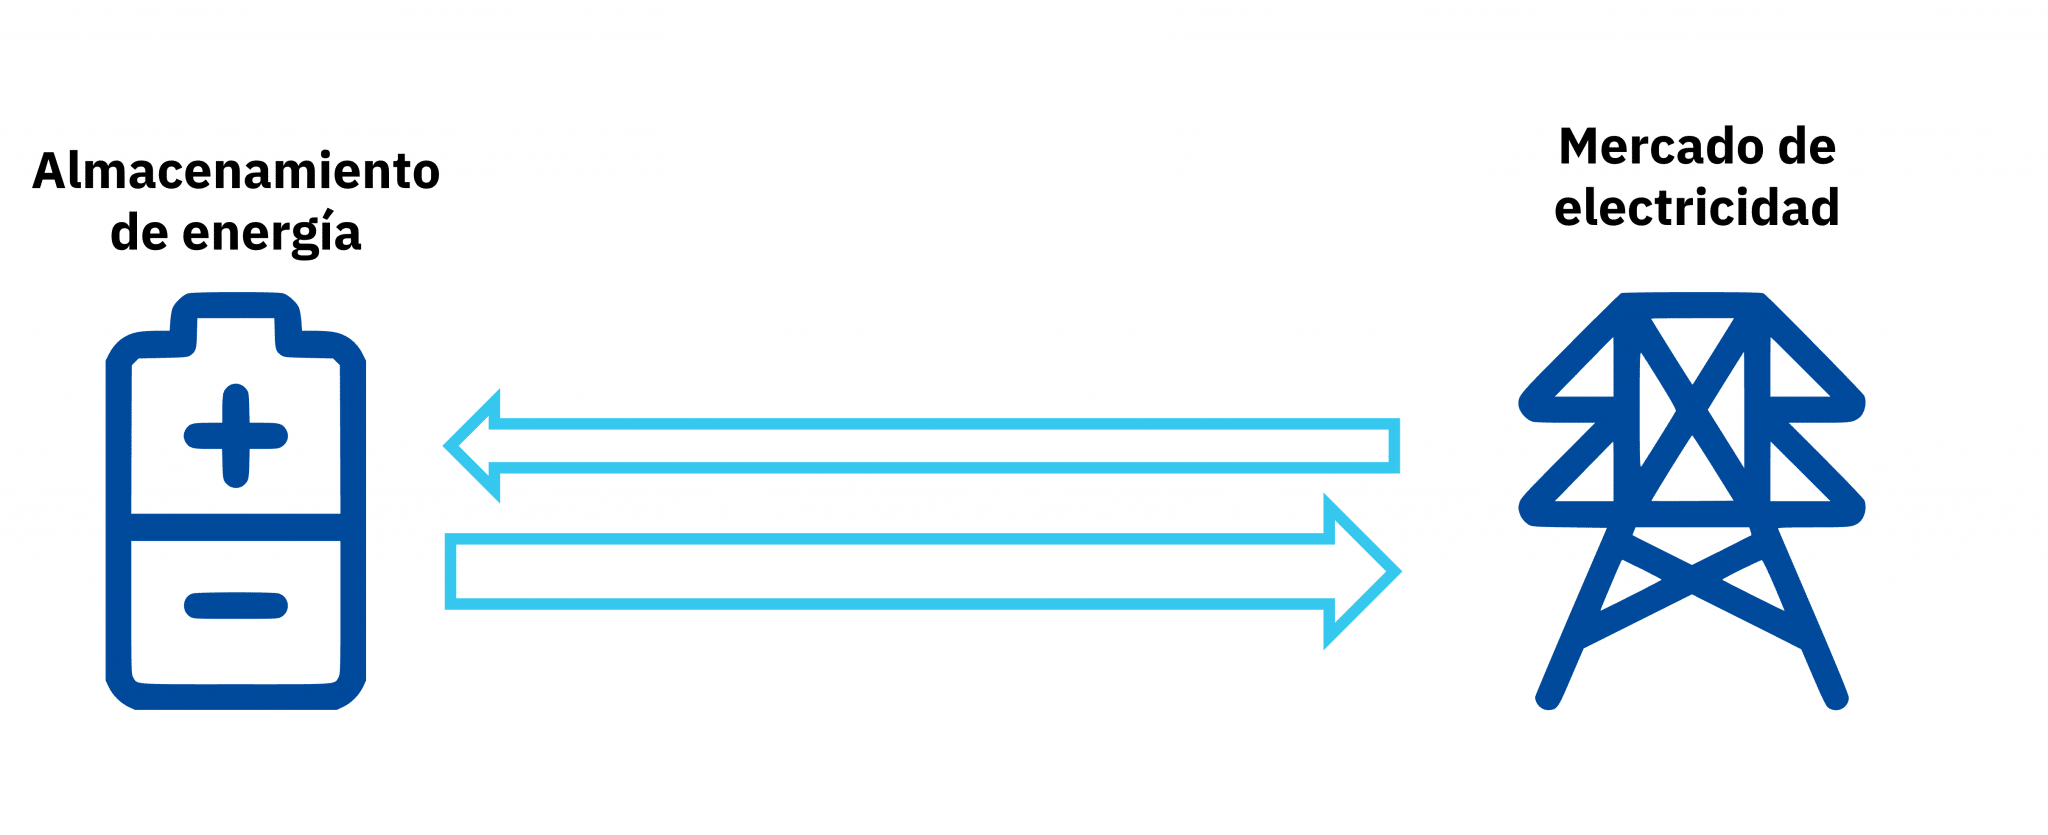
\includegraphics[width=0.5\linewidth]{figures/topologia-aislada.png}
  \caption[Diagrama de una instalación aislada.]{Diagrama de una instalación aislada con su activo de almacenamiento y sus correspondientes flujos energéticos~\cite{aleasoft2025la}.}
  \label{fig:topologia-aislada}
\end{figure}

Esto significa que la operación de un sistema de almacenamiento de energía en baterías aislado se centra puramente en el intercambio de energía con la red, lo que tan solo permite definir dos interfaces de flujo energético.

\begin{itemize}

  \item La interfaz de importación se corresponde al flujo de energía desde la red hacia el \gls{bess}. Este flujo comprende la única fuente de carga de la batería.

  \item  La interfaz de exportación representa el flujo de energía desde el \gls{bess} hacia la red. En contrapunto, se corresponde con la descarga de la batería.

\end{itemize}

De esta forma, esta topología es más común en las instalaciones energéticas principalmente dedicadas al negocio en los mercados de ajuste~\cite{carbajo2007mercados}, de tal forma que no necesiten encargarse del aprovechamiento energético de otros posibles activos energéticos dentro de la misma instalación.

Precisamente, uno de los ejemplos más representativos de esta topología en la actualidad es el \gls{bess} de Abadiño, en donde el negocio principal se realiza en los mencionados mercados de ajuste (las diferencias entre la situación actual y futura de las instalaciones standalone resulta especialmente interesante y es evaluada posteriormente en la sección~\ref{makereference7.3}).

A pesar de su aparente simplicidad, los análisis de mercado demuestran que la viabilidad económica de la topología aislada es limitada~\cite{azahra2020optimized, baviskar2023opportunities, kalenderova2024batery}.

El margen diferencial de precios, también conocido como \textit{spread}, entre las horas de bajo coste (valle) y alto coste (pico), a menudo resulta insuficiente para generar los ingresos necesarios que permitan amortizar la elevada inversión de capital y cubrir el \gls{capex} y \gls{opex}, incluyendo la degradación.

De hecho, para que estas instalaciones sean rentables, generalmente deben diversificar sus fuentes de ingresos mediante la participación activa en los dichos mercados de servicios de ajuste, como el \gls{afrr} y el \gls{mfrr}, teniendo que ofrecer disponibilidades de frecuencia y potencia.

Aunque la participación en estos mercados de regulación ofrezca una remuneración por la disponibilidad de capacidad, lo que se adapta perfectamente a la rápida respuesta de conmutación de las baterías, proporciona flujos de ingreso inestables de cara al futuro. Esto es debido al enorme crecimiento de la implantación de sistemas de almacenamiento de energía en baterías esperado, aumentando la oferta de disponibilidad y, por lo tanto, reduciendo a su vez las ganancias generadas individualmente por las baterías.

Cabe destacar que, aun teniendo una baja rentabilidad esperada, el sistema desarrollado soporta la configuración aislada sin ninguna complicación, al ser diseñado con una arquitectura modular en mente, capaz de adaptarse a, presuntamente, cualquier configuración topológica.

\subsection{Topología híbrida}
\label{makereference3.1.2}

Con el propósito de superar las limitaciones del modelo aislado y maximizar el aprovechamiento de la energía, han emergido con fuerza las configuraciones híbridas~\cite{bresciani2025hybridization}, el principal enfoque del sistema.

Estas topologías se definen por la llamada colocación del activo de generación, principalmente de generación renovable y generalmente fotovoltaica o eólica, con un \gls{bess}, como se muestra en la figura~\ref{fig:topologia-hibrida}.

\begin{figure}
  \centering
  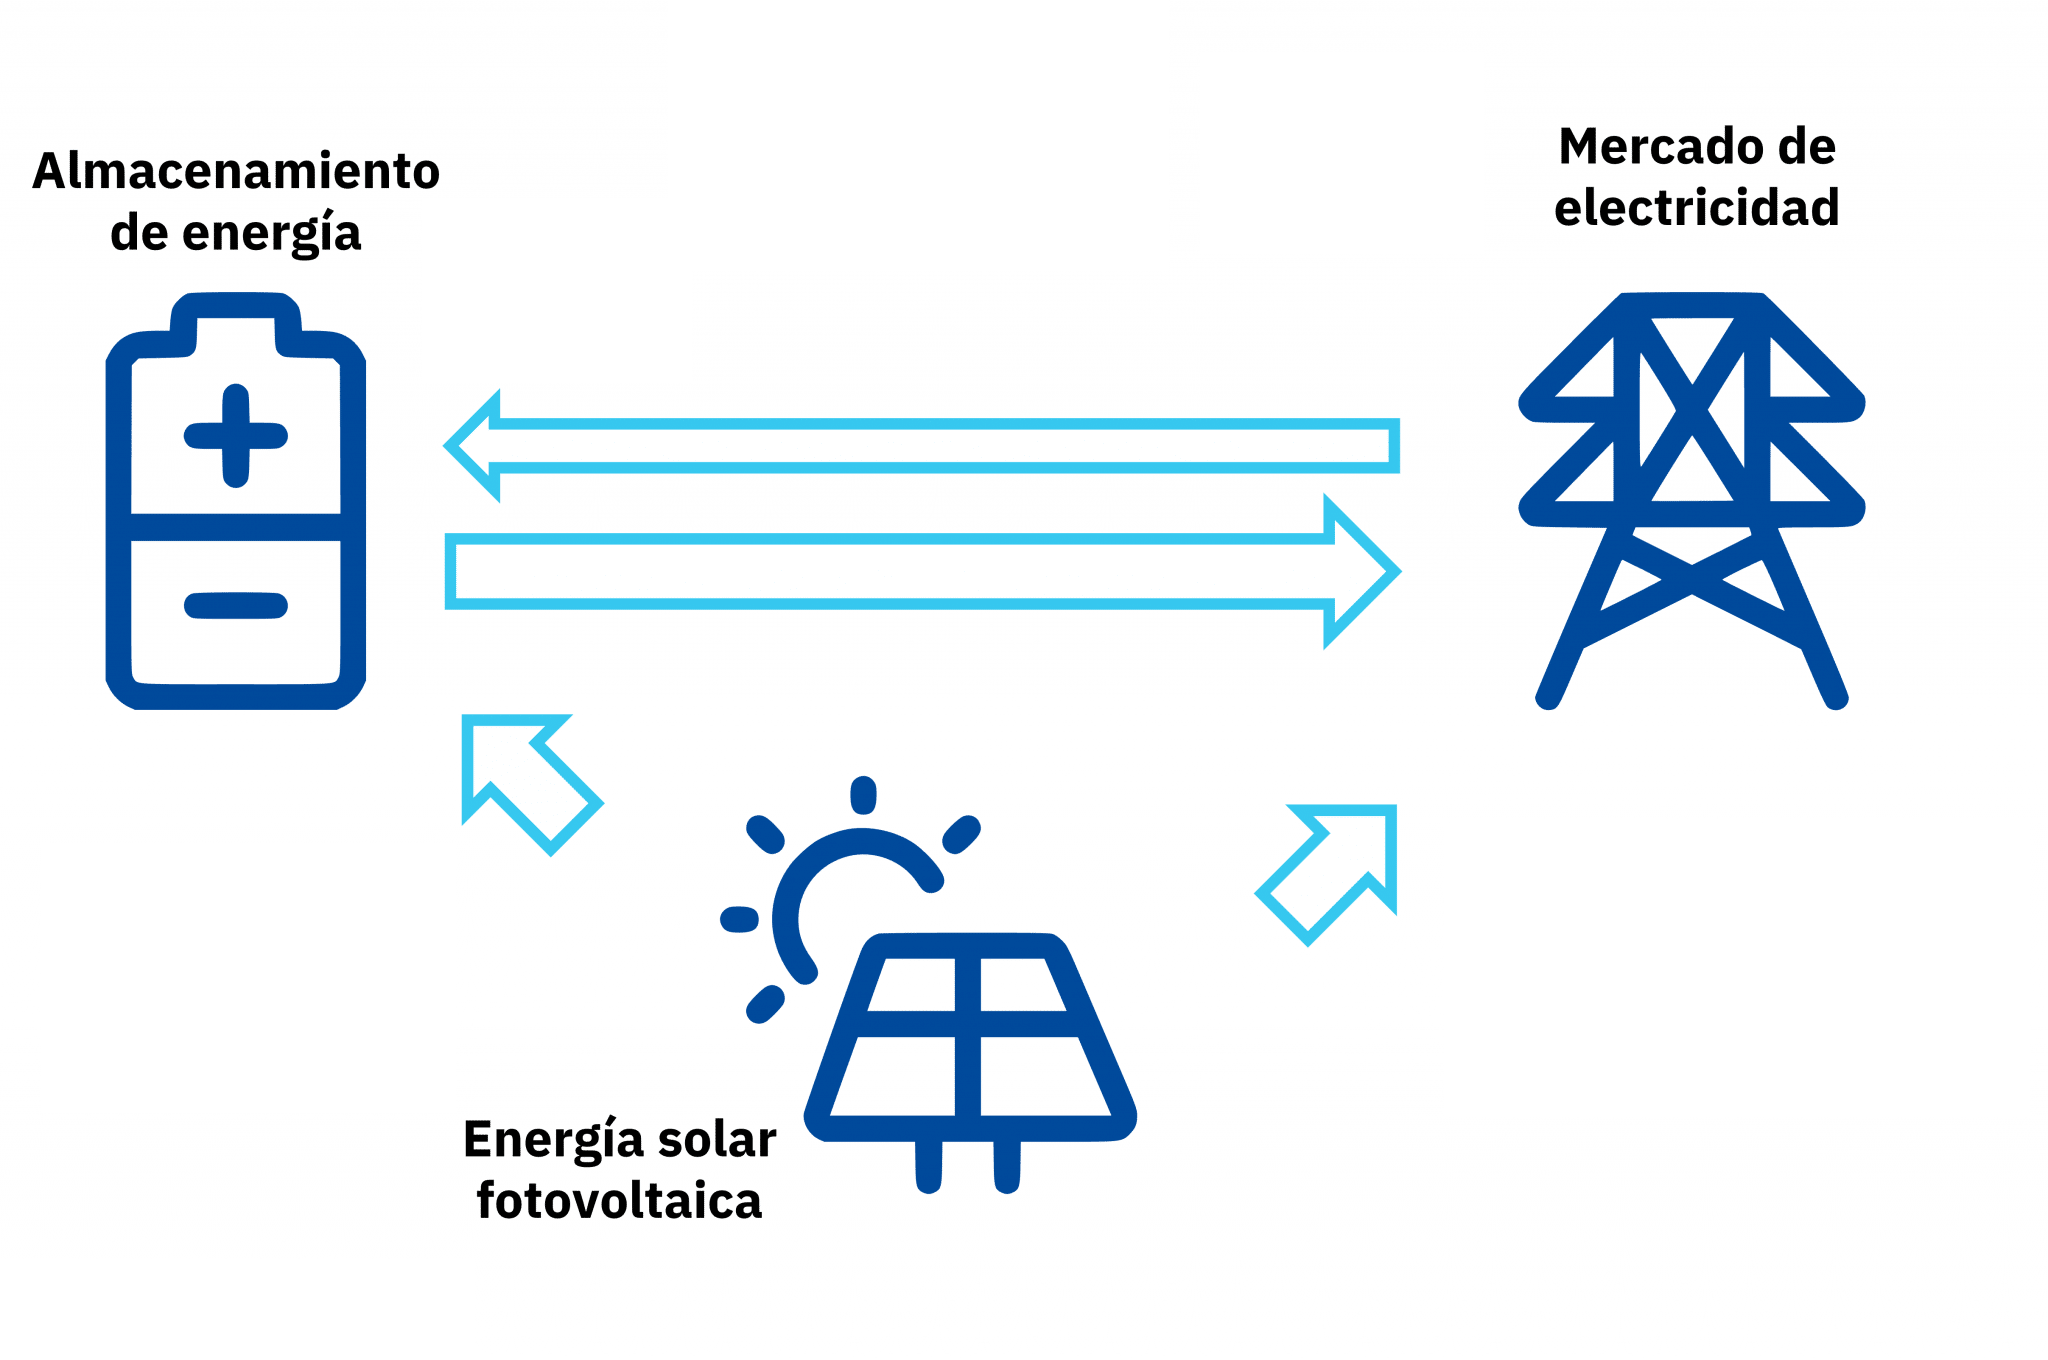
\includegraphics[width=0.5\linewidth]{figures/topologia-hibrida.png}
  \caption[Diagrama de una instalación híbrida.]{Diagrama de una instalación híbrida con sus activos de almacenamiento y generación y sus correspondientes flujos energéticos~\cite{aleasoft2025la}.}
  \label{fig:topologia-hibrida}
\end{figure}

Aunque los activos energéticos compartan ambos el mismo \gls{pf}, desde donde importan o exportan la energía a la red eléctrica, la batería es capaz de operar mediante lo que se conoce como \textit{behind the meter}. Esto es porque el flujo energético se mantiene dentro de la red interna de media tensión, sin volcarse necesariamente a la red pública de alta tensión.

\begin{itemize}

  \item Las interfaces de importación se corresponden tanto al flujo de energía desde la red hacia el \gls{bess} como al flujo energético desde la generación energética al \gls{bess}. Más allá de posibles restricciones estructurales u operativas, el sistema desarrollado debe ser capaz de diferenciar y seleccionar correctamente el canal de importación más adecuado según la situación analizada.

  \item Las interfaces de exportación representan, por un lado, el flujo de energía desde el \gls{bess} hacia la red, y por el otro, el flujo de energía desde la generación energética a la red. Como se tratan de dos activos energéticos separados, el desarrollo debe tenerlos en cuenta a los dos a la hora de realizar el arbitraje y dar la opción de comunicar no solo los resultados de la batería, sino también los de la generación, al estar enlazados entre sí, como se detalla en la sección~\ref{makereference5.3}.

\end{itemize}

Esta capacidad de carga interna transforma bastante notablemente el modelo operativo. Sin embargo, el término de hibridación mismo no describe un modelo único, ya que las restricciones operativas varían entre instalaciones, lo cual exige una flexibilidad muy grande por parte del funcionamiento del sistema desarrollado.

Por ello, la herramienta identifica y soporta de forma genérica las siguientes operaciones de la topología híbrida.

\begin{description}

  \item[Híbrida flexible] La configuración más versátil. El sistema de control tiene total libertad para decidir la fuente de carga (red eléctrica o generación energética) basándose exclusivamente en el criterio óptimo del algoritmo de control, que principalmente se trata de la maximización del beneficio. La instalación híbrida fotovoltaica y de almacenamiento de Puertollano es un arquetipo de este modelo.

  \item[Híbrida con prioridad de carga de generación] Opera bajo una restricción no económica, es decir, debe sacrificar beneficio para cumplir con las limitaciones del funcionamiento físico de la instalación. Una norma operativa de naturaleza física, aunque también pueda ser contractual o regulatoria, obliga al \gls{bess} a absorber toda la energía generada por la planta antes de poder cargar desde la red. La planta de híbrida eólica y de almacenamiento de Urkilla ejemplifica este tipo de limitación.

  \item[Híbrida con carga aislada de la red] Representa el escenario más restrictivo. La interfaz de importación desde la red para la carga del \gls{bess} está física o lógicamente deshabilitada, siendo la planta renovable asociada la única fuente de carga. Este modelo limita la operación a estrategias de autoconsumo de la producción renovable, donde se puede llegar a reservar parte de la generación para la batería. La instalación híbrida fotovoltaica y de almacenamiento de Campo Arañuelo es una representación de esta configuración.

\end{description}

La hibridación, incluso en sus formas más restrictivas, ofrece ventajas comparativamente altamente decisivas. Resulta que permite maximizar el valor de la energía renovable, almacenando excedentes que de otro modo se verterían a coste nulo. Además, al cargar desde la fuente renovable local, se evitan los costes regulatorios asociados al uso de la red pública~\cite{mterd2024orden} (peajes y cargos como el IVPEE, el bono social o las subvenciones del operador del sistema), lo que representa un ahorro directo y sustancial que mejora drásticamente los márgenes de arbitraje.

\section{Instrumentación de campo}
\label{makereference3.2}

La instrumentación de campo constituye el conjunto de dispositivos físicos que actúan como la interfaz directa entre los flujos energéticos. Por un lado, se encargan de medir con precisión las variables físicas clave (como la potencia, tensión, \gls{soc}, etc.) y por otro, son los actuadores que ejecutan las órdenes generadas por la lógica de control y optimización.

Concretamente, a partir dichos componentes, \gls{bms}, \gls{pcs}, transformador de medida y \gls{rtu}, ofrecidos por entidades como CATL~\cite{catl2023catl} e Ingeteam~\cite{ingeteam2025ingeteam}, el sistema extrae las siguientes señales.

\begin{description}

  \item[Estado de carga] Indica el porcentaje de energía en la batería. Es la variable más crítica para la toma de decisiones de carga y descarga. Expresado en porcentaje y megavatios hora\footnote{Dependiendo de la batería, aún todas siendo del mismo fabricante, es expresado de un modo u otro, por alguna razón.} y ofrecido por el \gls{bms}.

  \item[Estado de salud] Representa la capacidad actual de la batería en comparación con su capacidad nominal, reflejando su nivel de degradación a lo largo del tiempo. Expresado en porcentaje y megavatios hora\footnotemark[\value{footnote}] y ofrecido por el \gls{bms}.

  \item[Límites de potencia de carga y descarga local] Potencia máxima que el sistema de almacenamiento de baterías puede admitir o entregar en un momento dado, la cual puede estar limitada por factores internos como la temperatura. Expresados en megavatios y ofrecido por el \gls{bms}.

  \item[Disponibilidad] Señalización de la disponibilidad del estado interno de la batería, en forma de la cantidad de módulos o conjunto de celdas de carga disponibles en un momento dado, dependiendo de posibles fallos en la operación del sistema de almacenamiento. Expresado en porcentaje y ofrecido por el \gls{bms}.

  \item[Programa] El valor de consigna que el \gls{bms} está intentando seguir actualmente. Expresado en megavatios y ofrecido al \gls{bms}.

  \item[Potencia activa de carga y descarga] Medida en tiempo real de la potencia neta que se está inyectando o absorbiendo de la red. Expresado en megavatios y ofrecido por el \gls{pcs}.

  \item[Potencia activa de importación y exportación] La medición física de la potencia bruta que fluye a través del punto frontera, siempre dentro de la red de media tensión. Expresado en megavatios y ofrecido por los transformadores de medida.

  \item[Límites de potencia de descarga global] La máxima potencia de descarga que la planta puede ofrecer en su conjunto, la también llamada potencia estructural, que debe ser comunicada previamente al \gls{tso} por consideraciones legales. Expresados en megavatios y ofrecido por el \gls{rtu}.

  \item[Modo de control actual] Indica si la planta opera siguiendo las consignas externas señalizadas por el sistema a través del programa, o automáticamente por su cuenta según modos de funcionamientos internos no usados en el proyecto. Ofrecido por el \gls{rtu} y se fija en el seguimiento del programa.

\end{description}

De tal forma, estas son las señales de entrada y salida comunicadas a través de los protocolos de comunicación descritos en la siguiente sección~\ref{makereference3.3}, las cuales deparan en el sistema de información de planta de la sección~\ref{makereference3.4} tras ser adecuadamente configuradas.

\section{Protocolos de comunicación}
\label{makereference3.3}

Una vez los sensores han medido las variables físicas, los datos deben transmitirse de manera fiable y estructurada generalmente hasta la plataforma central o, en este caso, al \gls{pis}.

Para ello es necesario llevar a cabo una correcta selección de los protocolos de comunicación industriales a utilizar, siendo esta una de las tareas realizadas en el ámbito de la comunicación fuera de los activos de la instalación interna.

El principal desafío en entornos industriales es la interoperabilidad, siendo esta la capacidad de los diferentes dispositivos de intercambiar información sin ambigüedades. Por eso, los protocolos de comunicación son las reglas que actúan como el formato común para lograr esta necesaria interoperabilidad.

De esta forma, el \gls{pis}, explicado más adelante en la sección~\ref{makereference3.4}, debe entablar un vínculo con el controlador de planta o \gls{rtu}, concretamente. Pero, a la misma vez, el \gls{rtu} mismo necesita interactuar con el resto de activos físicos si pretende controlarlos de forma precisa.

Esa es la razón de la exposición de múltiples protocolos, y es que la comunicación entre los activos energéticos y el \gls{rtu} se realiza mediante Modbus TCP de forma agnóstica al sistema desarrollado, mientras que la comunicación entre el \gls{rtu} y el \gls{pis} es a través de IEC 60870-5-104.

\begin{figure}
  \centering
  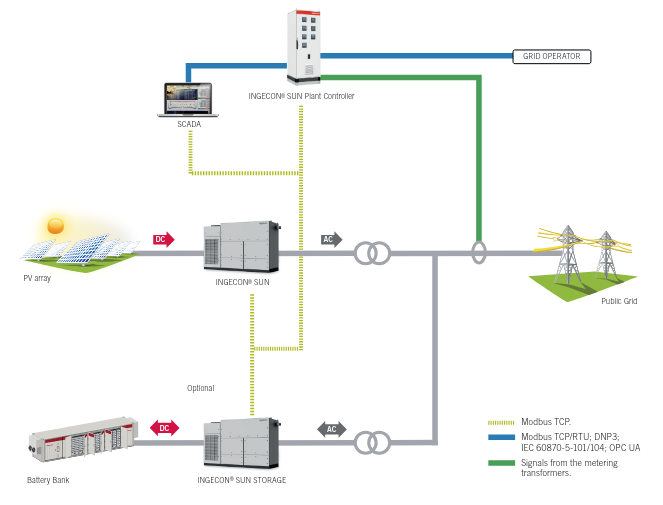
\includegraphics[width=0.5\linewidth]{figures/instrumentacion-de-campo.png}
  \caption[Diagrama de instrumentación de campo.]{Diagrama de la interacción entre los dispositivos y sensores físicos de campo.}
  \label{fig:instrumentacion-de-campo}
\end{figure}

\subsection{Modbus TCP}
\label{makereference3.3.1}

Modbus es uno de los estándares de facto en la automatización industrial por su simplicidad. Generalmente, es considerado uno de los estándares de comunicación industrial más ampliamente soportados~\cite{swales1999open}.

El protocolo sigue un modelo de comunicación conocido como maestro-esclavo, donde un dispositivo cliente (maestro) inicia las transacciones enviando peticiones a los dispositivos servidores (esclavos) para leer o escribir datos. Permite la interacción simple con sus relés, registros de entrada, registros de consigna y entradas discretas.

Los servidores responden a estas peticiones, asegurando un intercambio de información estructurado y fiable. Modbus TCP es precisamente ampliamente utilizado para la comunicación en la industria, al utilizar, como su propio nombre indica, el protocolo de capa de transmisión TCP/IP internamente. Ventajosamente, no requiere de lazos físicos entre los activos.

Dentro de la arquitectura del sistema, el protocolo Modbus TCP es utilizado para la comunicación interna entre los activos energéticos de la instalación, como los \glspl{bess} y los \glspl{pcs}, y la \gls{rtu}. Esta elección, realizada por el integrador de la infraestructura física ajeno al desarrollo, se debe a su amplia adopción por parte de los fabricantes de equipos industriales y a su facilidad de implementación.

\subsection{IEC 60870-5-104}
\label{makereference3.3.2}

El estándar IEC 60870-5-104 es un protocolo de comunicación diseñado específicamente para el telecontrol y la automatización de sistemas de energía eléctrica, lo que se adecúa perfectamente al caso de uso pertinente~\cite{iec2016telecontrol}.

Actúa como una extensión del protocolo IEC 60870-5-101 y lo adapta para la comunicación a través de redes TCP/IP, simplificando su despliegue.

A diferencia de Modbus, este protocolo permite una comunicación orientada a eventos y no solicitada o espontánea, donde un dispositivo subordinado (servidor) puede enviar datos al sistema de control (cliente) sin una petición previa, lo cual es crucial para la notificación inmediata de alarmas o cambios de estado.

IEC 60870-5-104 también permite enviar señalizaciones de calidad correspondientes a un valor, de hecho, es relativamente común ver señales sobrepasando los limites operacionales, como el estado de carga de una batería obtenido a mediante el protocolo observado en la figura~\ref{fig:overflow-soc}. Por suerte, estas señalizaciones de calidad permiten identificarlas, junto a valores inválidos, no actualizados, manuales, bloqueados o erróneos.

\begin{figure}
  \centering
  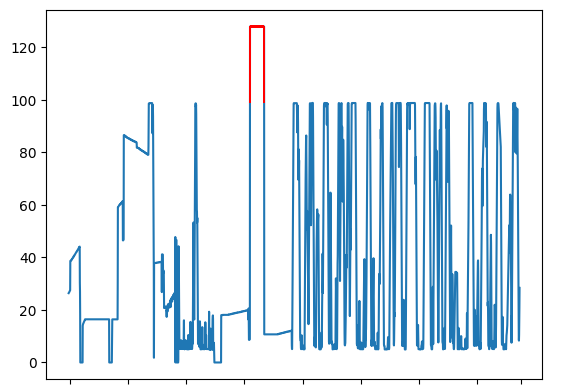
\includegraphics[width=0.5\linewidth]{figures/overflow-soc.png}
  \caption[Estado de carga excedente.]{Los valores del estado de carga excedente con respecto al limite operativo son registrados como inválidos por el protocolo.}
  \label{fig:overflow-soc}
\end{figure}

Con esto, se debe mencionar que el sistema desarrollado hace uso tanto de las señales a través de \textit{polling}, como de las señales espontáneas (asíncronas), aunque de forma más reducida en el caso de estas últimas. Concretamente, estas son configuradas para dar opción a la herramienta de optimización a conocer señales relacionadas con la disponibilidad de los recursos, y es que puede que el \gls{bess} haga saltar una alarma en caso de que se pierdan suficientes módulos de carga para afectar a la disponibilidad.

En el contexto del sistema desarrollado, el protocolo IEC 60870-5-104 es el canal de comunicación principal entre el \gls{rtu}, que actúa como servidor IEC 60870-5-104, y el \gls{pis}, que actúa como cliente. Esta comunicación es fundamental para transmitir los datos operativos de los activos energéticos al historiador de datos y, a su vez, para enviar las consignas de operación, los comandos de carga y descarga, desde el sistema de optimización hacia la planta.

Precisamente, la elección absolutamente fundamental del uso del protocolo IEC 60870-5-104 se realiza debido no solo a la capacidad de mensajería orientada a eventos, sino, principalmente, a las consideraciones de cumplimiento con los estándares impuestos por la institución dueña de la red eléctrica pública, el \gls{tso}, parte de sus funciones detalladas según su identificador conocido como \gls{asdu} en la tabla~\ref{tab:funciones-de-aplicacion-red}.

Ellos detallan el uso del protocolo para garantizar la respuesta con respecto al intercambio de información de la red. Por lo tanto, el sistema desarrollado se limita a seguir con la utilización de los estándares impuestos. De esta forma, se muestran para enfatizar el razonamiento industrial real por detrás de la decisión tomada del uso de IEC 60870-5-104, el cual está incluso ratificado oficialmente en España~\cite{une2017equipos}.

\begin{table}[ht]
  \centering
  \begin{tabular}{|l|p{7.5cm}|l|l|}
    \hline
    ASDU & Descripción                                               & Mnemónico   & Prioridad \\
    \hline
    103  & Sincronización del reloj                                  & C\_SC\_NA\_1 & Alta     \\
    147  & Programa de consumo                                       & M\_PC\_AA    & Baja     \\
    149  & Datos de tiempo real (Consumo)                            & M\_TR\_AA    & Baja     \\
    155  & Datos de tiempo real (Generación)                         & M\_TR\_GN    & Baja     \\
    169  & Orden de reducción de potencia                            & C\_PR\_IK    & Alta     \\
    180  & Petición de programa de consumo o de parada/mantenimiento & C\_PC\_AA    & Baja     \\
    182  & Petición de datos de tiempo real                          & C\_TR\_AA    & Baja     \\
    \hline
  \end{tabular}
  \caption[Funciones de aplicación para la comunicación con la red eléctrica.]{Extracto de las funciones de aplicación asociadas definidas por el operador del sistema de transporte para la comunicación del sistema con la red eléctrica, consolidadas en el llamado \gls{sceci}~\cite{ree2009protocolo}. El sistema hace uso de sus propias funciones de aplicación asociadas, comunicadas en última instancia a la red a través aquí mostrados.}
  \label{tab:funciones-de-aplicacion-red}
\end{table}

\section{Sistema de información de planta}
\label{makereference3.4}

Conociendo ya tanto los activos físicos disponibles, de los cuales obtener los datos sensoriales, como los canales de comunicación, es necesario ofrecer una interfaz de interacción bidireccional entre la herramienta principal que realiza la optimización operativa y la infraestructura física.

Para esta función crítica, la arquitectura del sistema se apoya en parte de la infraestructura preexistente del \gls{pis} desplegado.

Precisamente, en muchas arquitecturas de sistemas industriales reales en producción, la totalidad de la información entrante y saliente de los activos físicos pasa por el sistema SCADA\@. En cambio, aunque en la arquitectura general del desarrollo propio sí que tenga cabida uno de esos sistemas, la comunicación con los activos físicos es realizada sin ningún tipo de indirección secundaria, significando que el sistema SCADA queda fuera del alcance y no es pertinente al diseño realizado. Es decir, la información fluye directamente al \gls{pis} sin pasar por el SCADA\@, aunque exista un sistema SCADA externo.

\subsection{Contextualización del sistema}
\label{makereference3.4.1}

De esta forma, el \gls{pis} seleccionado se trata del llamado PI System de AVEVA (antes OSIsoft), una plataforma tecnológica diseñada para la gestión de datos de operaciones en tiempo real a escala industrial, que viene como anillo al dedo al caso de uso del sistema~\cite{aveva2025aveva}.

Su núcleo principal, el PI Server, actúa como un repositorio centralizado que no solo almacena, sino que también enriquece y contextualiza los extensos flujos de datos de series temporales provenientes de la instrumentación de campo.

Si bien el componente del servidor en concreto ya se encontraba desplegado, entendiblemente para controlar el resto de instalaciones no relacionadas con los \gls{bess}, su alcance no se extendía a la monitorización y control de los activos energéticos específicos pertinentes al desarrollo realizado, las instalaciones con activos de almacenamiento, concretamente.

Por lo tanto, una contribución fundamental resulta ser el diseño, la implantación y la configuración detallada de los canales de comunicación bidireccionales usando los componentes descritos anteriormente para integrar estos activos, detallado el diseño en la figura~\ref{fig:sistema-de-informacion-de-planta}.

\begin{figure}
  \centering
  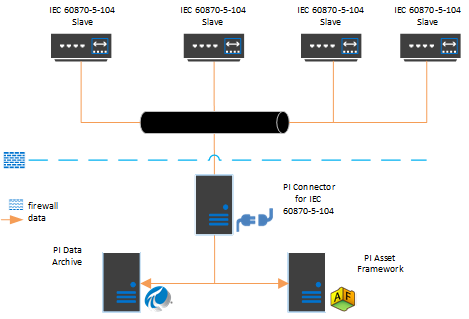
\includegraphics[width=0.5\linewidth]{figures/sistema-de-informacion-de-planta.png}
  \caption[Arquitectura del sistema de información de planta.]{Arquitectura de los canales de comunicación del sistema de información de planta~\cite{aveva2025aveva}.}
  \label{fig:sistema-de-informacion-de-planta}
\end{figure}

Para ello, se ha desplegado el PI Connector para IEC 60870-5-104, un componente de software que actúa como traductor entre el protocolo de telecontrol estándar del sector eléctrico y el ecosistema del PI System, también mostrado en la figura.

\subsection{Consideraciones de seguridad}
\label{makereference3.4.2}

Es bien sabido que las consideraciones de seguridad no son una característica más de los sistemas críticos industriales que controlan activos energéticos, sino que deben ser tomados como requerimientos fundamentales.

Por ello, el proceso de puesta en marcha requiere de una configuración precisa para garantizar, por una parte, la integridad de los datos y, por otra, su seguridad. Con esto, el conector es desplegado en un servidor Windows Server 2022 dedicado dentro de una llamada \gls{idmz}, asegurando la independencia y seguridad de las comunicaciones.

Las \gls{idmz} se encuentran entre las redes de \gls{ot} y de \gls{it} y se diferencian en que deben intentar asegurar la disponibilidad y los tiempos de respuesta de los procesos físicos industriales que alojan. Esto se traduce en que no se alojan necesariamente cerca de las fuentes de datos de campo, ni directamente junto al resto de servicios informacionales, sino que deben existir en las localizaciones relacionadas con la sala de control que supervisa el funcionamiento correcto de dichos servicios con por lo menos una seguridad mínimamente mayor.

Como tanto el conector como el servidor del \gls{pis} se encuentran en la misma \gls{idmz} y no en una red \gls{ot} en contrapunto a la red \gls{it}, no es necesario introducir otra capa de indirección. Esta capa actuaría como intermediario seguro para respetar las políticas de seguridad entre las redes, pero eso significa que debe existir un control en forma de \textit{firewall} más avanzado aún entre redes para que la herramienta de optimización pueda acceder al historiador (el \gls{pis}), en forma del llamado PI Relay. Aún así, gracias a la arquitectura usada, no es necesario introducir esta complejidad añadida a costa del aisaliento total entre redes (se sigue manteniendo el aislamiento necesario).

De esta forma, se observa que, en concreto, el despliegue del conector, actuando como \textit{gateway} entre el protocolo de comunicación y el historiador de datos, y precisamente el historiador de datos mismo, se encuentran posicionados en el nivel 3.5 de la zona desmilitarizada industrial de la \gls{pera}, el cual define un modelo estructural estandarizado para la seguridad de los sistemas de control industrial.

\begin{figure}
  \centering
  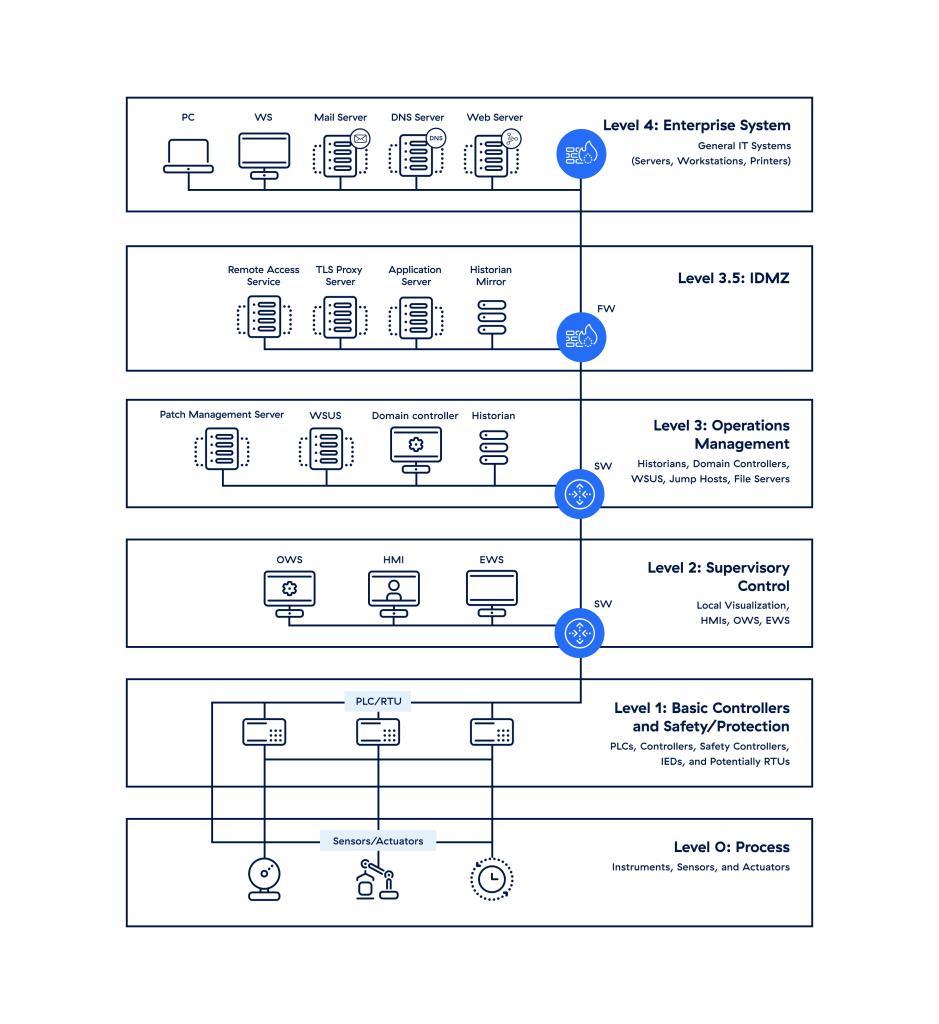
\includegraphics[width=0.5\linewidth]{figures/modelo-purdue.png}
  \caption[Modelo Purdue.]{Modelo Purdue para la seguridad de los sistemas de control industrial~\cite{zscaler2025what}.}
  \label{fig:modelo-purdue}
\end{figure}

\subsection{Configuración funcional}
\label{makereference3.4.3}

La parametrización del conector, junto con la especificación de parte la lógica de traducción a llevar a cabo, se ha realizado mediante el administrador del conector mostrado en la figura~\ref{fig:administador-del-conector}.

\begin{figure}
  \centering
  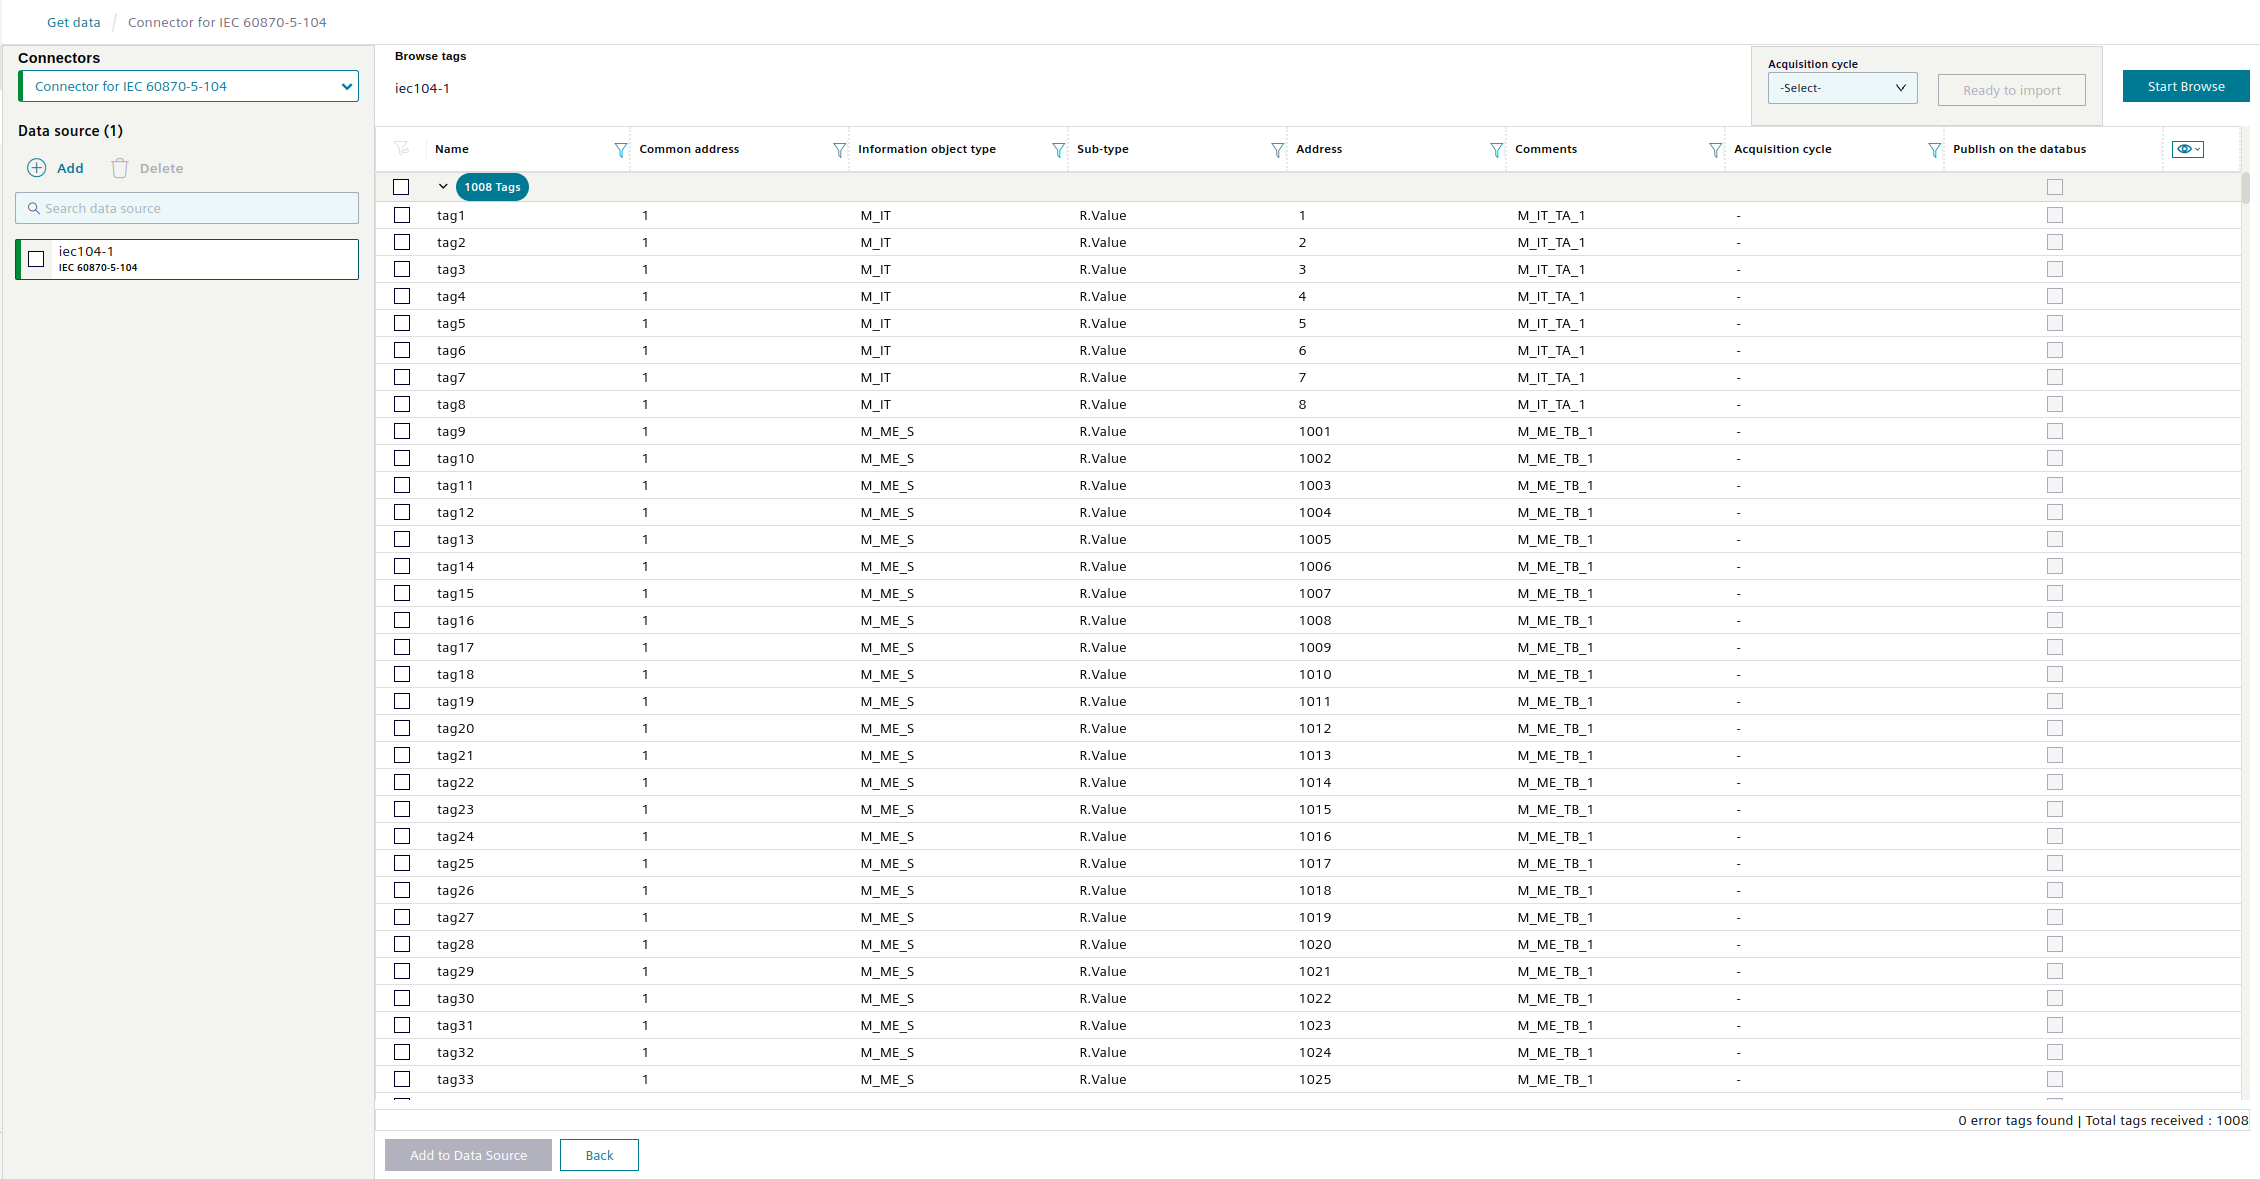
\includegraphics[width=0.75\linewidth]{figures/administador-del-conector.png}
  \caption[Interfaz del administrador del conector.]{Interfaz del administrador del conector mostrando el descubrimiento de señales del dispositivo subordinado.}
  \label{fig:administador-del-conector}
\end{figure}

Por la parte de la selección del PI Server al cual transmitir los datos, se especifica la dirección IP y el puerto del mismo. En concreto, el tipo de servidor se debe corresponder con la tecnología de archivado del historiador usada, la cual resulta ser PI Data Archive, a diferencia de PI Asset Framework de más alto nivel.

Desde la perspectiva de la fuente de datos, se requiere introducir la localización del dispositivo primario subordinado de IEC 60870-5-104.

Junto a ello, se ajustan los parámetros clave del protocolo en sí, como las \glspl{asdu}, que identifican unívocamente a la estación. Para facilitar el descubrimiento, es posible enviar un comando de \gls{gi} utilizando la \gls{asdu} 0xFFFF que devuelva todos los canales encontrados en el dispositivo subordinado, y filtrarlos posteriormente.

A su vez, para garantizar un tiempo de respuesta razonable, se configuran también los temporizadores del protocolo. El temporizador \( t_1 \) determina el timeout de la confirmación de datos enviados, el \( t_2 \) el timeout de envío del reconocimiento si no se han enviado datos nuevos, y el \( t_3 \) el timeout de inactividad de la conexión.

Como el servicio de ajuste obligatorio (no remunerado) con menor granularidad es de 30 segundos máximo, es decir, se deben enviar pulsos que cubran el 50 \% de la regulación en menos de 15 segundos y el 100 \% en menos de 30 segundos para controlar la batería~\cite{cnmc2024balance}, es necesario aplicar valores menores o iguales a dichos tiempos a los temporizadores \( t_1 \) y \( t_2 \), 4 segundos según recomendaciones, concretamente.

Es importante recalcar que aunque la menor granularidad a la que deben trabajar las baterías sea tan baja, el sistema desarrollado nunca necesitará de un tiempo de respuesta tan rápido, ya que controla el arbitraje de batería en mercados de más alta granularidad (mayor o igual a 15 minutos). Tan solo se modifican los temporizadores para, de forma ajena al desarrollo, tener la opción de habilitar los sistemas de almacenamiento de energía en batería no solo para el uso del sistema propio, sino para el negocio simultaneo en los mercados auxiliares previamente descritos y servicios de regulación, que son los que disponen de esta granularidad reducida.

Finalmente, intentando asegurar la sincronización de los sensores y evitar la perdida de información, la periodicidad de la \gls{gi}, comando esencial del protocolo que solicita una actualización completa de todos los puntos de datos, se define en 1 hora. Esto es debido a que este valor se corresponde con el intervalo mínimo entre la negociación de dos mercados, lo que es diferente de la granularidad del mercado. Aún así, los búferes de transmisión de las unidades remotas permiten disminuir notablemente la perdida de datos. Esto es relevante ya que el sistema de control de planta no realiza peticiones bajo demanda a los dispositivos, sino que devuelve el valor ya al almacenado.

\begin{figure}
  \centering
  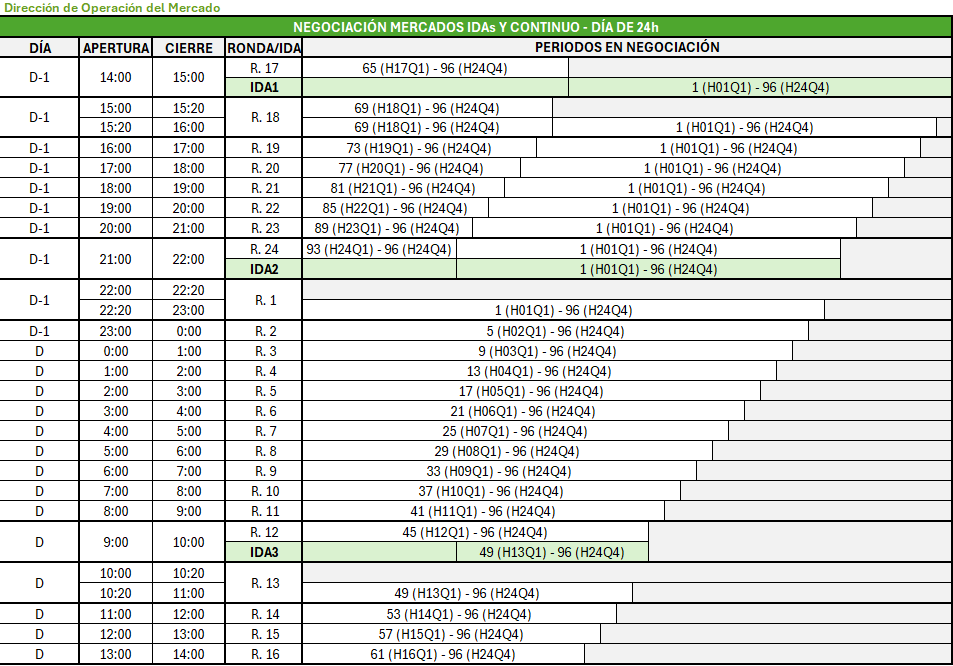
\includegraphics[width=0.75\linewidth]{figures/tiempo-mercados.png}
  \caption[Calendario de negociación de los mercados eléctricos.]{Calendario de negociación de los mercados eléctricos intradiarios y continuo~\cite{omie2025mercado}.}
  \label{fig:tiempo-mercados}
\end{figure}

Más allá y tal y como se ha descrito anteriormente, es posible aprovechar las capacidades de mensajería orientadas a eventos del protocolo para no tener que enviar comandos de \gls{gi} continuamente. No importa no tener datos estrictamente actualizados para las señales relacionadas con los parámetros operativos del \gls{bess}, pero sí que importa no estar actualizados en cuanto a su disponibilidad estructural. Es decir, parámetros como el \gls{soc}, la energía almacenada, la potencia de carga o descarga, etc.\ son modelados intrínsecamente en el funcionamiento de la instalación, en cambio, los fallos estructurales no lo son (pueden ocurrir en cualquier momento, el resto tienen comportamientos predecibles). Por suerte, una vez configurada la relación con los puntos de la conexión, el conector es capaz de recibir estas señales espontaneas automáticamente aprovechando el funcionamiento del protocolo.

De esta forma y una vez establecido el enlace de comunicación, el conector procede al descubrimiento de las señales disponibles, interrogando al controlador de planta y presentando una lista completa de los objetos de información accesibles, cada uno identificado por su dirección de objeto de información.

Se seleccionan únicamente las variables críticas para la operación de la batería y la planta de generación asociada, correspondientes a las señales de los sensores anteriormente descritos en la sección~\ref{makereference3.2}. Posteriormente, se debe realizar un mapeo explícito de cada \gls{ioa} seleccionada a un elemento de datos en el PI Server. Para cada señal, se crea un PI Point correspondiente en el PI Data Archive, definiendo sus atributos como tipo de dato (\texttt{Float32} para mediciones continuas, \texttt{Digital} para descripciones de estado), unidades de ingeniería (\si{\percent}, \si{\mega\watt}, \si{\mega\watt\hour}), un descriptor textual claro y el identificador correspondiente (\texttt{BT SOC Real}, etc.). Es posible visualizar el resultado en la figura~\ref{fig:visualizacion-industrial-de-batería}.

\begin{figure}
  \centering
  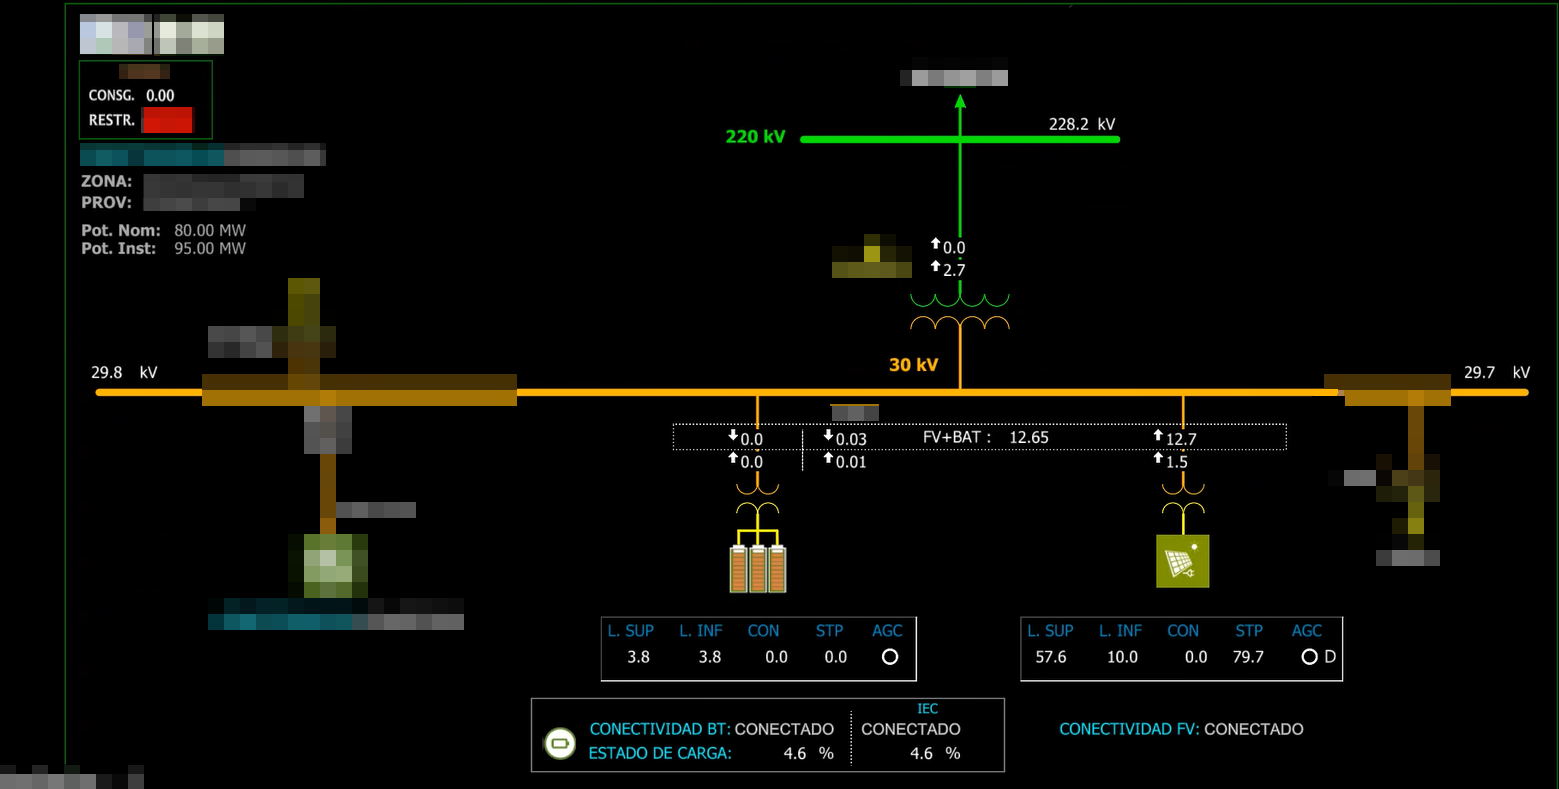
\includegraphics[width=0.75\linewidth]{figures/visualizacion-industrial-de-bateria.png}
  \caption[Visualización industrial de señales de instalación.]{Visualización industrial de varias señales de una instalación.}
  \label{fig:visualizacion-industrial-de-bateria}
\end{figure}

Como no se hace uso de PI Asset Framework para modelizar la planta de forma jerárquica, se definen los identificadores de cada punto según sus características. Los valores analógicos (analog value) siguen el formato \texttt{M:06X.AV}, las calidades analógicas (analog quality) \texttt{M:06X.AQ}, los valores de las consignas (setpoint value) \texttt{M:06X.SV} y las calidades de las consignas (setpoint quality) \texttt{M:06X.SQ}. Se muestra una colección de los mismos en la tabla~\ref{fig:puntos-bateria}.

\begin{figure}
  \centering
  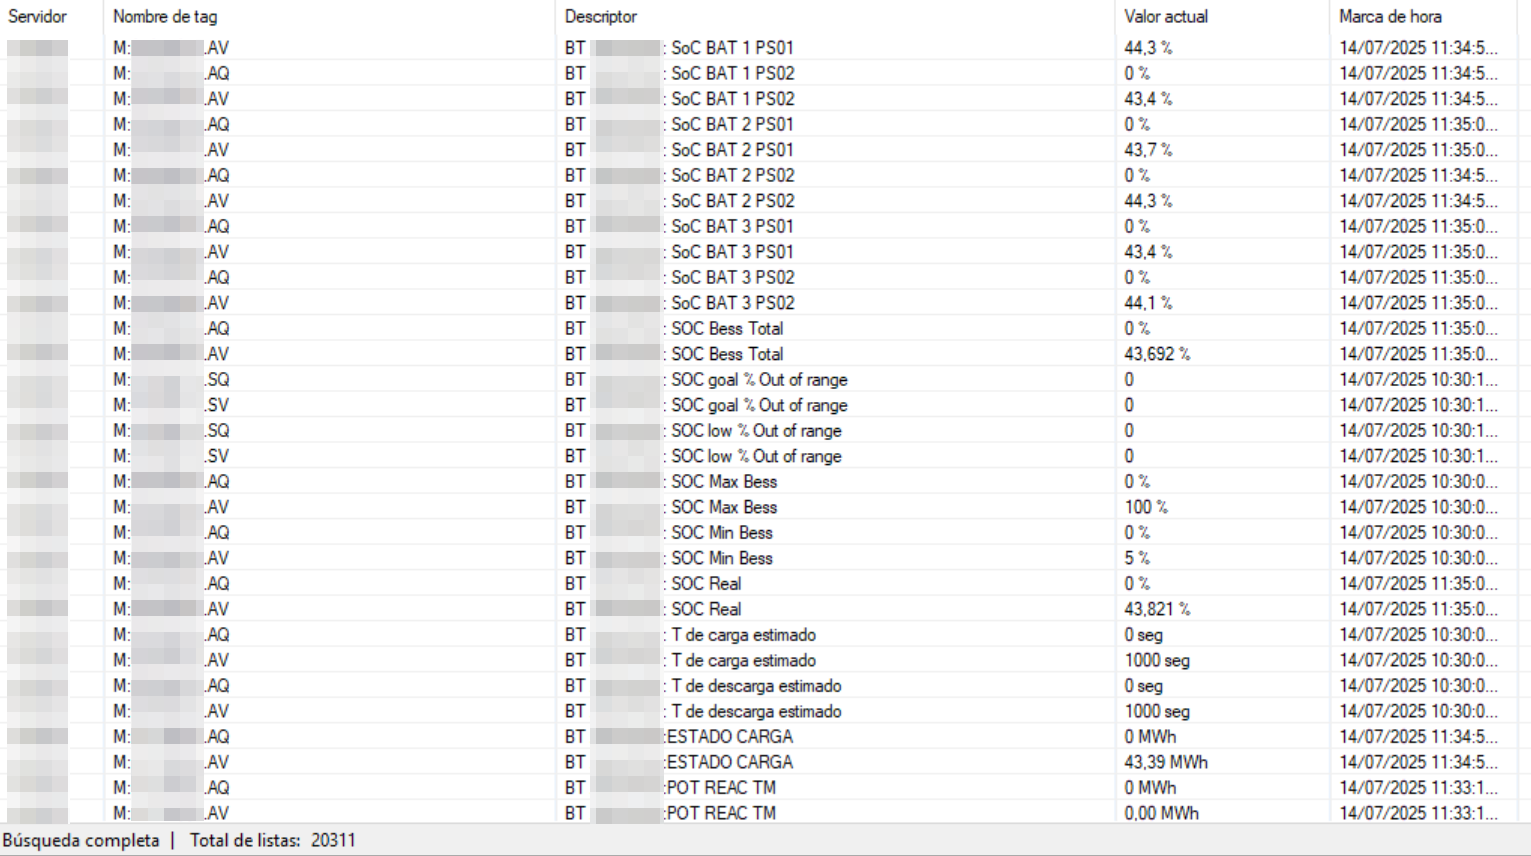
\includegraphics[width=0.75\linewidth]{figures/puntos-bateria.png}
  \caption[Colección de puntos de una batería.]{Colección de puntos de una batería.}
  \label{fig:puntos-bateria}
\end{figure}

Los valores, como su nombre indica, se corresponden con el contenido de las señales, sean continuas o no. Las calidades, en cambio, representan la salud de las señales definido por el protocolo y son usadas para filtrar malas señales.

Con ello, la validación del sistema se realiza comparando en tiempo real los valores registrados en el PI Data Archive con las lecturas directas en la interfaz SCADA de los controlador de planta en la respectiva sala de control securizada, y forzando cambios en los activos para verificar la correcta transmisión y registro de eventos. De esta forma, es posible comparar el programa de carga y descarga de las baterías con los movimientos verdaderamente efectuados y comprobar su corrección, como se muestra en la figura~\ref{fig:programa-bateria}.

\begin{figure}
  \centering
  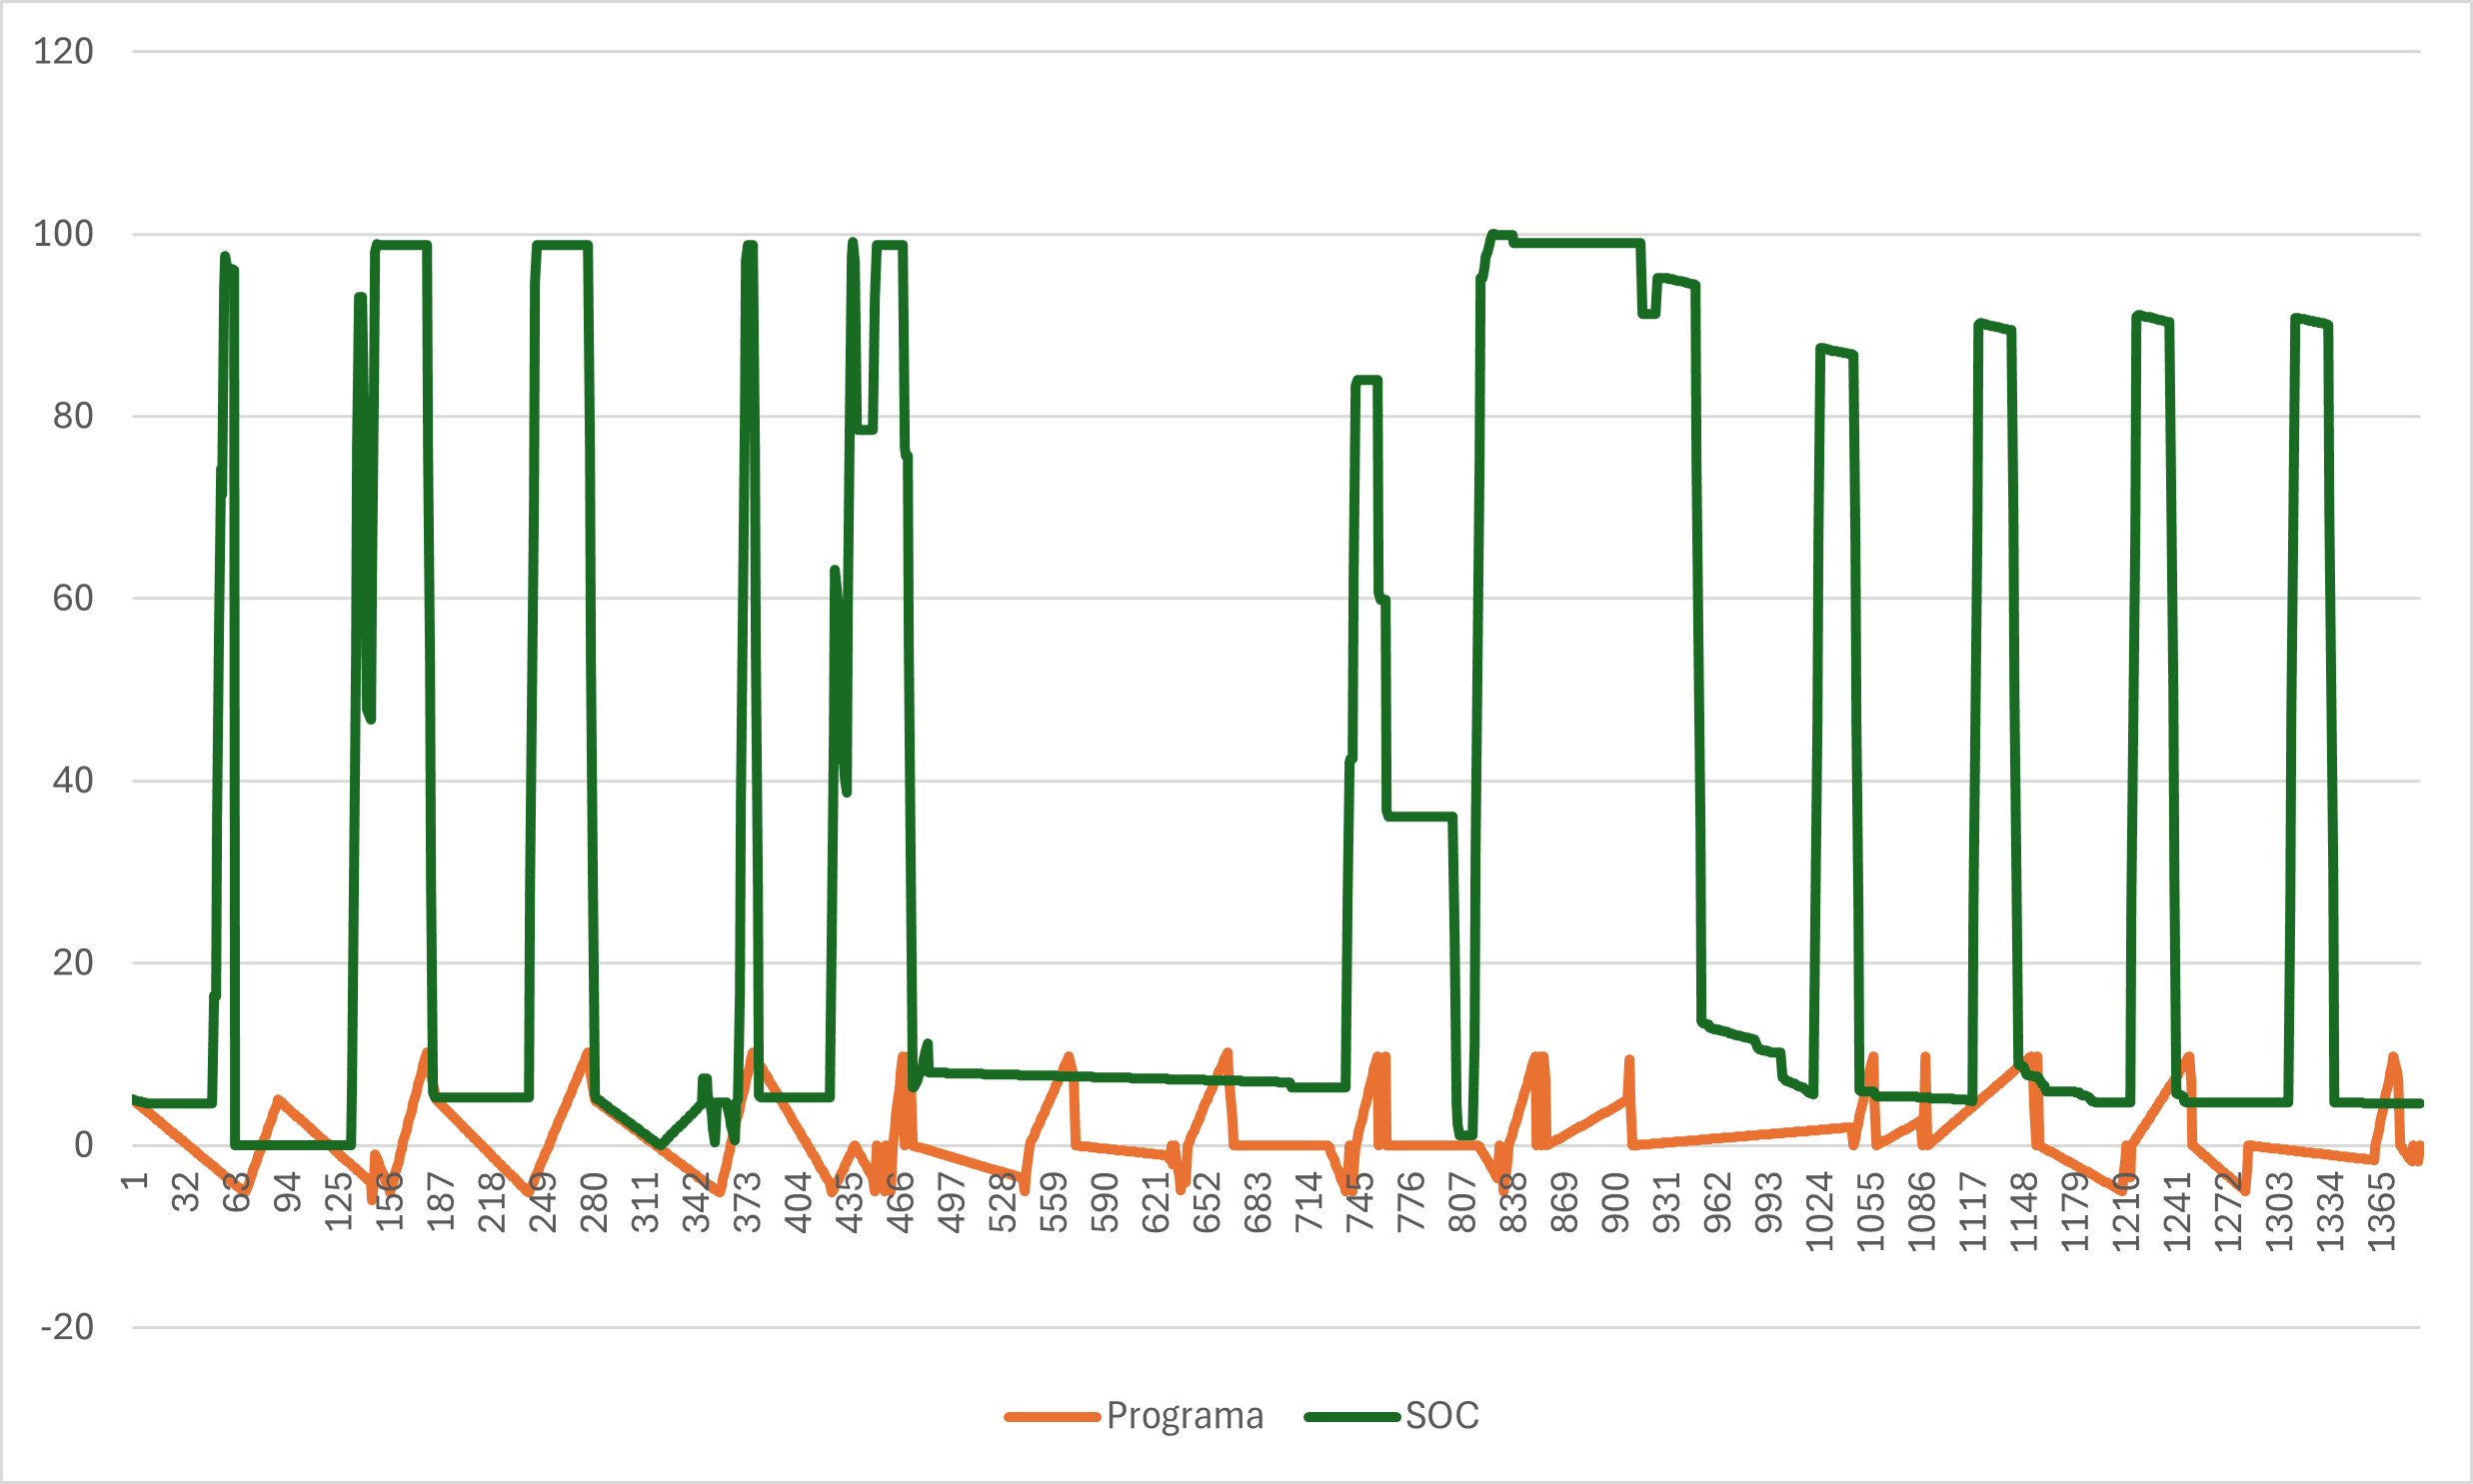
\includegraphics[width=0.75\linewidth]{figures/programa-bateria.png}
  \caption[Programa de ciclado de una batería.]{Programa de ciclado de una batería en comparación con su evolución del estado de carga.}
  \label{fig:programa-bateria}
\end{figure}

Precisamente, esta validación permite determinar múltiples errores en la lógica de consignación, De hecho, durante la validación se consiguieron corregir múltiples fallos más o menos críticos.

Uno de ellos, el hecho de olvidarse bajar la potencia de las baterías al mínimo técnico tras el mandato de una señal de carga, error que precisamente causa una carga excedente de la baterías durante el periodo de pruebas correspondiente a una perdida monetaria puntual del calibre de miles de euros netos.

Otra situación interesante fue dada por el método de actualización de las señales de \textit{polling} y las espontaneas, como la disponibilidad. Como la disponibilidad es actualizada nada más cambiar, por consideraciones de reporte, puede que no se encuentren sincronizadas con las otras señales. Para resolverlo, se ponen en acuerdo la disponibilidad y el resto de señales relacionadas con la misma una vez se haya realizado la petición.

Por suerte, el sistema de control de baterías no permite el incorrecto funcionamiento de las baterías desde la perspectiva física y hace sonar la alarma ante tales situaciones, actualizando su disponibilidad, por lo que la batería no sufre ningún daño aunque no se disponga de recurso energético en periodos de carga.

\section{Consumo del historiador}
\label{makereference3.5}

Una vez que la infraestructura de adquisición y almacenamiento ha sido configurada y validada, y los datos operativos de los activos fluyen de manera fiable hacia el historiador, el siguiente paso es establecer los mecanismos para su consumo.

Precisamente, el consumo no se limita a una simple lectura de valores brutos, sino que abarca la transformación de algunas de las métricas para la obtención de valores dependientes, como los rendimientos del ciclo, y la interfaz programática que conecte el historiador con la herramienta de optimización, intentando hacer frente a posibles incompatibilidades tecnológicas entre ambas plataformas.

\subsection{Ecuaciones de rendimiento}
\label{makereference3.5.1}

Para representar valores dependientes con significado físico, en vez de tener que consultar múltiples puntos simultáneamente para inferir el resultado computado de los mismos, resulta más conveniente y efectivo el uso de las ecuaciones de rendimiento proporcionadas como parte del PI System.

Las ecuaciones de rendimiento o PI Performance Equations son una solución eficaz para detallar la lógica de señales calculadas de forma similar a la definición previa de los puntos. Precisamente, la diferencia principal es la introducción de la ecuación misma y el evento de actualización, ya que se requiere conocer de que puntos depende la ecuación para poder recomputarla cuando estos cambien.

\begin{figure}
  \centering
  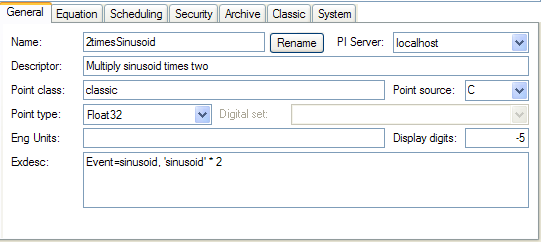
\includegraphics[width=0.5\linewidth]{figures/ecuaciones-de-rendimiento.png}
  \caption[Creación de una ecuación de rendimiento.]{Creación de una ecuación de rendimiento.}
  \label{fig:ecuaciones-de-rendimiento}
\end{figure}

Mediante las ecuaciones de rendimiento se detallan los siguientes puntos.

\begin{itemize}

  \item El rendimiento de carga, que afecta a la energía importada y define la cantidad de energía perdida durante la carga de la batería. Su razón de ser es el ajuste de los posibles desvíos a la hora de comprar energía que surgirían si no se tuvieran en cuenta las perdidas. El rendimiento de carga es calculado mediante la simple relación entre la energía importada y energía cargada \( \eta_{c} = E_{\text{imp}} / E_{c} \).

  \item El rendimiento de descarga, que afecta a la energía exportada y define la cantidad de energía perdida durante la descarga de la batería. Es necesaria para el ajuste de los posibles desvíos a la hora de vender energía si no se tuvieran en cuenta las perdidas. El rendimiento de descarga es calculado mediante la simple relación entre la energía exportada y energía descargada \( \eta_{d} = E_{\text{exp}} / E_{d} \).

\end{itemize}

\subsection{Integración programática}
\label{makereference3.5.2}

Finalmente, teniendo los datos provenientes de tanto de los activos físicos disponibles en el historiador como de sus propias transformaciones, es necesario consumirlos por la herramienta principal de optimización con el propósito de conocer los parámetros operativos de las baterías.

Para ello, existen múltiples enfoques que tomar, aunque el elegido a sido hacer uso de la interfaz de aplicación ofrecida por el PI AF SDK, la cual provee acceso estructurado a una variedad de componentes del PI System.

% TODO
\begin{figure}
  \centering
  % \includegraphics[width=0.5\linewidth]{figures/integración-programatica.png}
  \caption[Diagrama de componentes entre plataformas.]{Diagrama de componentes entre plataformas.}
  \label{fig:integración-programatica}
\end{figure}

Aún y todo, la librería expone su interfaz a través de Microsoft \.NET pero la herramienta de optimización ha sido desarrollada en Python, lo que resulta en un problema de incompatibilidad que podría no permitir el uso de PI AF SDK\@.

Para solucionar el problema principal de esta incompatibilidad, es posible utilizar la integración de Python con el \.NET Common Language Runtime, la máquina virtual que se encarga de ejecutar el código para la plataforma de \.NET\@. Esto se hace posible a través de los bindings de Python.NET\@.

Precisamente, se hace un uso directo de la interfaz a través del lenguaje de programación elegido para el apartado de la conexión con el PI Server. Y es que, en términos de la conexión, resulta que para cumplir con los requisitos de seguridad de la comunicación entre redes, los métodos de conexión por defecto recomendados no se pueden usar. En cambio, es necesaria la autenticación con credenciales directa, aunque esto suponga la perdida de la reconexión automática ofrecida por los métodos de conexión por defecto.

Junto a ello, con el propósito de aumentar la ergonomía del desarrollo, se toma la librería Piconnect, que ofrece una interfaz directa más simple y también hace uso internamente de la integración con la interfaz de \.NET, resultando en el diagrama de la figura~\ref{fig:integración-programatica}.

Con todo, los puntos son consumidos mediante los llamados valores registrados, significando un valor discreto en el tiempo, y valores interpolados, para obtener la evolución de los mismos a lo largo del tiempo. La comunicación de vuelta a los activos físicos es discutida más adelante en la sección correspondiente de comando y control~\ref{makereference6.1.1}.

% chktex-file 44

\cleardoublepage%

\chapter{Entorno de mercado}%
\label{makereference4}

Para que el sistema de optimización de baterías funcione de manera efectiva, no es suficiente con disponer de la información proveniente de la infraestructura con sus sensores y señales. Como el sistema opera directamente en el mercado eléctrico, su lógica de decisión debe ser retroalimentada por un entendimiento del entorno de mercado. Por ello, los datos de mercado son una fuente de información igualmente indispensable, ya que dictan el contexto económico y regulatorio en el que se toman todas las decisiones de arbitraje, formando parte de los componentes destacados del flujo de la figura~\ref{fig:esquema-mercado}.

\begin{figure}
  \centering
  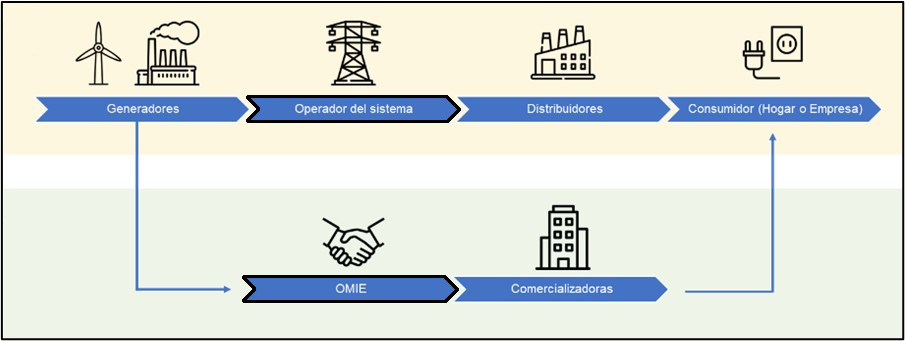
\includegraphics[width=0.75\linewidth]{figures/esquema-mercado.jpg}
  \caption[Esquema del funcionamiento del mercado.]{Esquema del funcionamiento del entorno del mercado, destacando las entidades regulatorias de las que obtener información~\cite{villagrasa2023como}.}%
  \label{fig:esquema-mercado}
\end{figure}

Por tanto, se define el análisis de las fuentes de información de mercado y los procesos desarrollados para su adquisición, tratamiento e integración. Concretamente, el sistema de optimización requiere de cuatro categorías fundamentales de datos externos. Los precios del mercado son esenciales para formular previsiones estratégicas. La energía negociada es clave para la liquidación de beneficios y la gestión de desvíos. Las limitaciones operativas imponen restricciones de obligado cumplimiento. La situación meteorológica indica las previsiones de la generación.

De esta forma, se pretende describir el origen de estas fuentes de datos, las reglas que gobiernan su publicación y acceso, y la arquitectura implementada para consumirlos de manera programática y robusta.

Con esto, para facilitar la comprensión de las secciones posteriores, se reiteran los siguientes conceptos. Las \glspl{ufi} son identificadores lógicos que definen los puntos de intercambio de energía. A diferencia de un punto físico en la red, una \gls{ufi} es una referencia contractual para las operaciones de mercado, con la condición indispensable de que toda transacción debe estar respaldada por un flujo de energía físicamente viable. Las \glspl{up} son los identificadores del \gls{tso} de las instalaciones al completo y resultan los activos que se arbitran en el mercado. Las \glspl{uof} son los identificadores equivalentes del \gls{mo}. Es decir, las operaciones de las \glspl{ufi} que engloba una \gls{up} o \gls{uof} se agregan a la hora de realizar la oferta.

Para ello, primeramente se presenta \gls{omie} como la fuente primordial de datos de mercado, detallando los mecanismos de obtención de precios y la naturaleza de la información de la energía negociada, como se describe en el apartado~\ref{makereference4.1}. A continuación, se habla de la información proveniente de \gls{ree}, que impone las limitaciones de programa de operación en tiempo real, como se explica en la sección~\ref{makereference4.2}. Finalmente, el apartado~\ref{makereference4.3} detalla como se consolidan estas diversas fuentes de datos para formar una visión unificada que sirva de entrada al sistema. El flujo de información del entorno de mercado se representa en la figura~\ref{fig:arquitectura-mercado}.

\begin{figure}
  \centering
  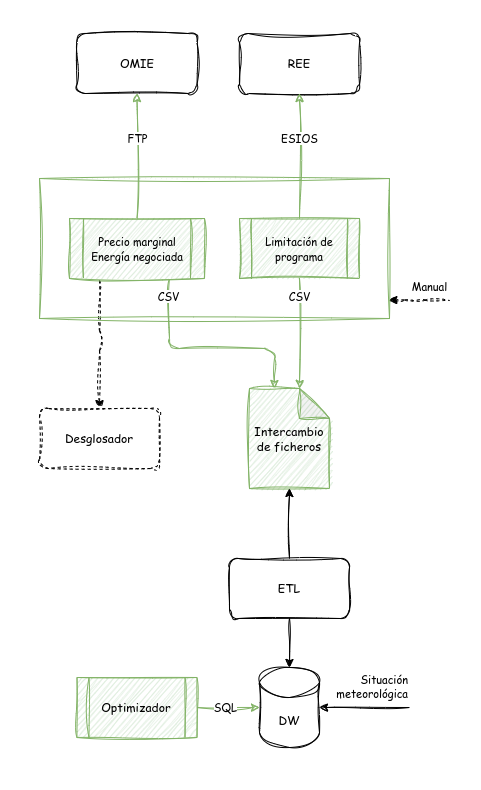
\includegraphics[height=0.7\textheight]{figures/arquitectura-mercado.png}
  \caption[Arquitectura del entorno de mercado.]{Arquitectura del flujo de información del entorno de mercado, diferenciando los elementos pertinentes al proyecto. Las tareas temporizadas según el horario de mercado de la obtención de datos de \gls{omie} y \gls{ree} obtienen los ficheros de precios marginales, energía negociada y limitaciones de programa a través de la plataforma FTP del \gls{mo} y ESIOS del \gls{tso}. Una vez se han consultado los desgloses de programa para transformar las unidades de \gls{up} a \gls{ufi}, se procesan las entradas y se depositan los resultados de las inserciones al \gls{dw} en el intercambiador de ficheros en formato CSV\@. Después de que un proceso \gls{etl} externo termine cargándolos en base de datos, estos son consultados por el optimizador mediante SQL, junto con la situación meteorológica. Se tiene en cuenta también la posibilidad de introducir información manualmente a las tareas de mercado, ante posibles contratiempos en las fuentes de información.}%
  \label{fig:arquitectura-mercado}
\end{figure}

\section{Operador del mercado}%
\label{makereference4.1}

\Gls{omie} es la institución responsable de la gestión de los mercados spot, diario, intradiarios y continuo de electricidad en la península ibérica. Actúa como la plataforma centralizada donde los agentes de mercado presentan sus ofertas de compra y venta de energía, y cuyo proceso de casación determina los precios y las cantidades de energía negociadas para cada periodo de negociación.

Por su rol como gestor y árbitro del mercado, \gls{omie} es la fuente oficial de toda la información relativa a los resultados económicos de la operación. Cualquier sistema que pretenda participar activamente en el arbitraje energético, como el desarrollado en este proyecto, tiene la necesidad de integrarse de forma fiable y programática con los flujos de información que esta entidad publica.

Precisamente, \gls{omie} pone a disposición la información en forma de ficheros publicados según un horario acordado tras el cierre de cada mercado correspondiente.

De esta forma, la información que el sistema desarrollado toma a través de \gls{omie} se clasifica en dos categorías mayoritarias, los precios marginales de casación y la energía finalmente negociada por unidad.

\subsection{Precio marginal}%
\label{makereference4.1.1}

Una de las piezas de información más críticas para el sistema de optimización es la previsión de los precios a los que se liquidará la energía en los mercados futuros. Para poder realizar un arbitraje energético efectivo, posicionando estratégicamente las ofertas de compra en periodos de bajo coste y las de venta en periodos de alto beneficio, el modelo debe operar sobre una estimación fiable de dichos precios, mostrados en la figura~\ref{fig:mercado-diario}.

\begin{figure}
  \centering
  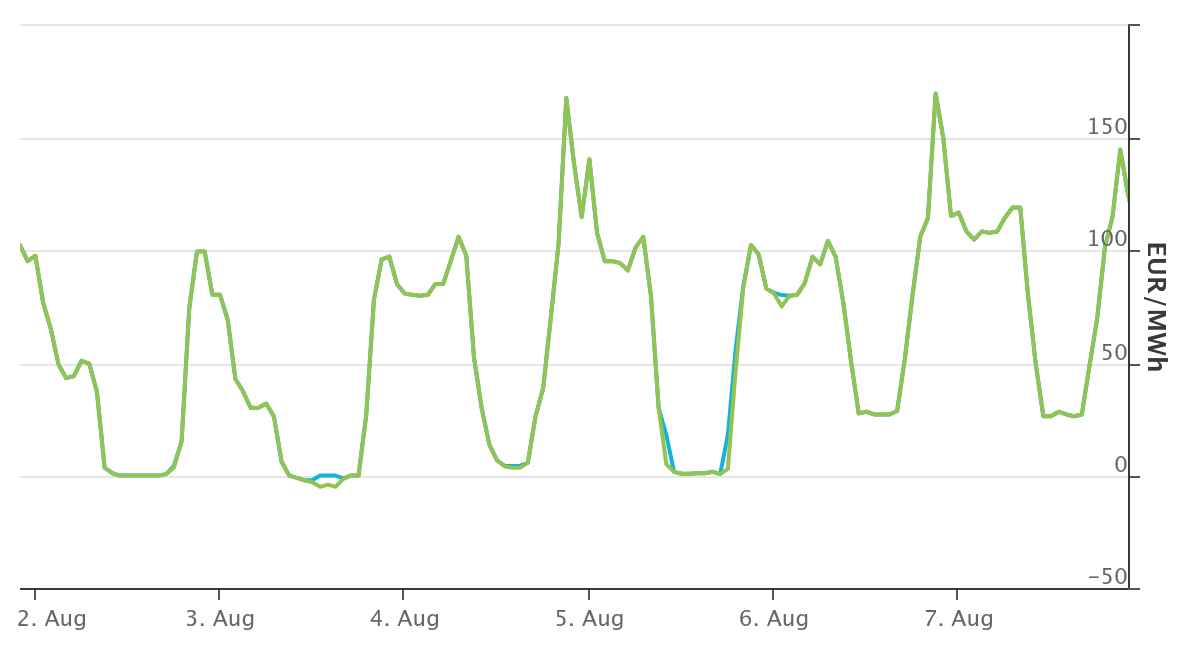
\includegraphics[width=0.75\linewidth]{figures/mercado-diario.png}
  \caption[Precio del mercado diario de la primera semana de agosto.]{Precio real del mercado diario de la primera semana de agosto, del cual se debe tener disponible una previsión para operar a futuro.}%
  \label{fig:mercado-diario}
\end{figure}

Precisamente, sin esta previsión, la operación de la batería sería puramente ciega sin ningún tipo de guiado ni garantía de corrección.

Por ello, para obtener esta previsión, el sistema desarrollado adopta un enfoque triple que se aprovecha de las características temporales de cada mercado.

\begin{description}

  \item[Mercado diario] La variabilidad de precios entre días es significativamente mayor al resto de mercados y depende de factores del entorno más complejos, como falta de lluvia, negociaciones de fin de semana, capacidades de interconexión, industria, estación del año, etc. De esta manera, el sistema está preparado para consumir previsiones de dos orígenes distintos. Por un lado, se utiliza un modelo de previsión manual en el que los agentes de mercado introducen sus propias estimaciones basadas en su experiencia. Por otro, se integra con un modelo de aprendizaje automático, concretamente un modelo de regresión de \textit{stacking} basado en series temporales, que ofrece una predicción automatizada. Dependiendo de la situación, es posible hacer uso de uno u otro\footnote{Se subraya que dichos modelos son externos al desarrollo.}.

  \item[Mercado intradiario] Se observa una alta correlación y una periodicidad estable entre sesiones consecutivas correspondida por lo agentes de mercado, por lo que se utiliza una previsión simple y efectiva donde el precio de casación de una sesión de mercado se emplea como la previsión para la sesión inmediatamente posterior. Así, por ejemplo, los precios resultantes del primer mercado intradiario sirven como la previsión para optimizar las ofertas del segundo, y así sucesivamente.

  \item[Mercado intradiario continuo] Se toma el precio de casación del último mercado disponible, sea el diario o intradiario. Cabe destacar que debido a la comparativamente baja liquidez del mercado continuo, la metodología de previsiones de precio descrita es la menos fiable para el mismo, aunque este aspecto negativo sea contrarrestado por la suma de liquidez total de las sesiones en conjunto del mercado continuo\footnote{Esto significa que, aunque la previsión de una de las sesiones del mercado intradiario continuo no atine, es posible recuperar los desvíos acumulando negociaciones en los mercados intradiarios continuos posteriores.}. La razón de este comportamiento es la diferente modalidad de oferta del mercado, donde se ataca directamente a una oferta, por lo que no existen precios de casación globales para todas ellas, sino individuales.

\end{description}

Afortunadamente, la información de precios de casación es de carácter público. \Gls{omie} la publica en ficheros con una nomenclatura estandarizada, siendo el fichero \gls{marginalpdbc} para el mercado diario y los ficheros marginales \gls{marginalpibci} para los mercados intradiarios~\cite{cnmc2025resolucion}.

\subsection{Energía negociada}%
\label{makereference4.1.2}

Más allá de las previsiones de precios, el sistema necesita conocer con absoluta certeza el resultado de las ofertas que ha presentado al mercado. Existe una diferencia fundamental entre la posición óptima calculada por el algoritmo de optimización y la posición casada, que es la cantidad de energía que la instalación se ha comprometido firmemente a comprar o vender.

Esto se debe a que el funcionamiento del mercado eléctrico permite negocia la energía de un mismo periodo en múltiples sesiones, por lo que hay que llevar la cuenta de la cantidad de energía anteriormente ofertada.

Por ello, obtener esta información de energía licitada es importante, porque permite realizar la liquidación económica real de la operación, calculando el beneficio o coste exacto a partir del precio marginal y la energía efectivamente negociada.

Además, es un requisito indispensable para la gestión de los desvíos y la reoptimización en mercados subsecuentes. Al conocer la energía ya comprometida, el modelo puede ajustar su plan para las siguientes sesiones, minimizando así las más costosas penalizaciones por desvío que se producen al no cumplir con el programa de energía comprometido.

Precisamente, esta discrepancia entre lo ofertado y lo casado puede deberse a múltiples factores, como que el precio de oferta no resulte competitivo y la oferta sea rechazada en su totalidad, o que se produzca una casación parcial en la que solo una fracción de la energía ofertada es aceptada por el mercado. Esta es la razón de la necesidad de tener que consultar con \gls{omie} y no poder fiarse de la posición optima obtenida del sistema.

Pero, a diferencia de los precios, la información de energía casada es de naturaleza confidencial. Para proteger las estrategias comerciales de los participantes en el mercado, \gls{omie} la publica desglosada por \gls{up}, y cada entidad solo tiene acceso a la información de sus propias unidades. Los ficheros que contienen esta información son el \gls{pdbf} para el mercado diario y el \gls{pibca} para los mercados intradiarios~\cite{cnmc2025resolucion}.

\section{Operador del sistema}%
\label{makereference4.2}

Mientras que \gls{omie} gestiona el componente económico del mercado, la responsabilidad de garantizar la seguridad y estabilidad física del sistema eléctrico en tiempo real recae sobre \gls{ree}. Como \gls{tso}, \gls{ree} tiene el rol fundamental de balancear constantemente la generación con la demanda y de operar la red de transporte de alta tensión de manera segura, evitando sobrecargas o colapsos.

Para cumplir con esta misión crítica, el resultado puramente económico de la casación del mercado gestionado por \gls{omie} debe ser supervisado y, en ocasiones, modificado por \gls{ree}. Esto se debe a que un programa de producción económicamente óptimo podría no ser físicamente viable debido a las limitaciones de la red. Por esta razón, \gls{ree} emite consignas operativas de cumplimiento necesario que se aplican sobre el resultado del mercado, conocidas como limitaciones de programa.

\subsection{Limitaciones de programa}%
\label{makereference4.2.1}

Las limitaciones de programa son limitaciones de potencia impuestas por \gls{ree} a los participantes del mercado para resolver congestiones en la red o garantizar la seguridad del suministro en tiempo real. Estas limitaciones representan un límite superior inviolable a la operación de los activos energéticos y, por tanto, constituyen una entrada fundamental para el sistema de optimización.

La necesidad de estas limitaciones surge cuando el programa de energía resultante del mercado provocaría una sobrecarga en alguna línea de la red de transporte o comprometería la estabilidad del sistema. En tales casos, \gls{ree} interviene emitiendo una consigna que reduce la potencia máxima que una o varias instalaciones pueden exportar a la red.

Es importante tener en cuenta que, si bien las restricciones de las limitaciones de programa son altamente criticas, existen medios externos para garantizar que no se sobrepasan si ocurre algún error en la operación del sistema desarrollado, por lo que la estabilidad de la red nunca podrá verse afectada por un simple incumplimiento de las consignas por parte del sistema.

Con esto, la información de estas limitaciones se publica (o no) con ``antelación suficiente al cierre de mercado''~\cite{mte2019resolucion}. Como entre sesiones de mercado apenas existe una diferencia de una hora, no es estrictamente necesario consultar las limitaciones constantemente, sino tan solo antes de realizar la optimización.

Las limitaciones son desglosadas según diferentes identificadores.

\begin{itemize}

  \item Una limitación a nivel de \gls{ufi} de ls instalación aplica un límite de exportación de potencia a un activo de generación o almacenamiento específico e individual. Por ejemplo, podría limitar la producción de una planta fotovoltaica concreta dentro de un complejo más grande.

  \item Una limitación a nivel de \gls{up} impone un límite de exportación al conjunto de activos que conforman dicha \gls{up}. En una instalación híbrida, esto significa que la suma de la potencia neta exportada por la planta de generación y el \gls{bess} no puede superar el umbral dictado.

\end{itemize}

Por tanto, el sistema de optimización desarrollado debe consultar la existencia de estas limitaciones de programa, de la misma forma que la información anterior. Si se recibe una limitación, el modelo debe considerarla como una restricción máxima en sus cálculos, ajustando la consigna de operación de la batería para asegurar que la exportación total de las unidades se mantengan siempre por debajo del límite impuesto por \gls{ree}. El fichero de limitaciones de programa se conoce como \gls{limitacionsuj}.

\section{Situación meteorológica}%
\label{makereference4.3}

Además de las señales económicas de \gls{omie} y las operativas de \gls{ree}, existe una tercera fuente de datos externos que resulta indispensable para el sistema de optimización, concretamente en el caso de las topologías híbridas. Esta se trata de la previsión de la generación eléctrica que producen los activos de de generación (generalmente renovable) asociados a los sistemas de almacenamiento, dependientes de la situación meteorológica.

La necesidad de esta información es bastante directa, facilitando al sistema de optimización la toma de decisiones informadas sobre si cargar la batería desde la red o desde la generación. Por ello debe conocer con antelación cuánta de generación estará disponible en cada periodo. Sin esta previsión, la capacidad de la batería para aprovechar la energía generada localmente, uno de los principales beneficios económicos de la hibridación, sería nula.

Este proceso de previsión es una tarea externa al sistema desarrollado. Se basa en modelos especializados que toman como entrada previsiones meteorológicas (como la irradiancia solar, nubosidad, temperatura o velocidad del viento) y las traducen en una previsión de potencia para cada periodo del horizonte de optimización, cuyo resultado se muestra en la figura~\ref{fig:prevision-generacion}.

\begin{figure}
  \centering
  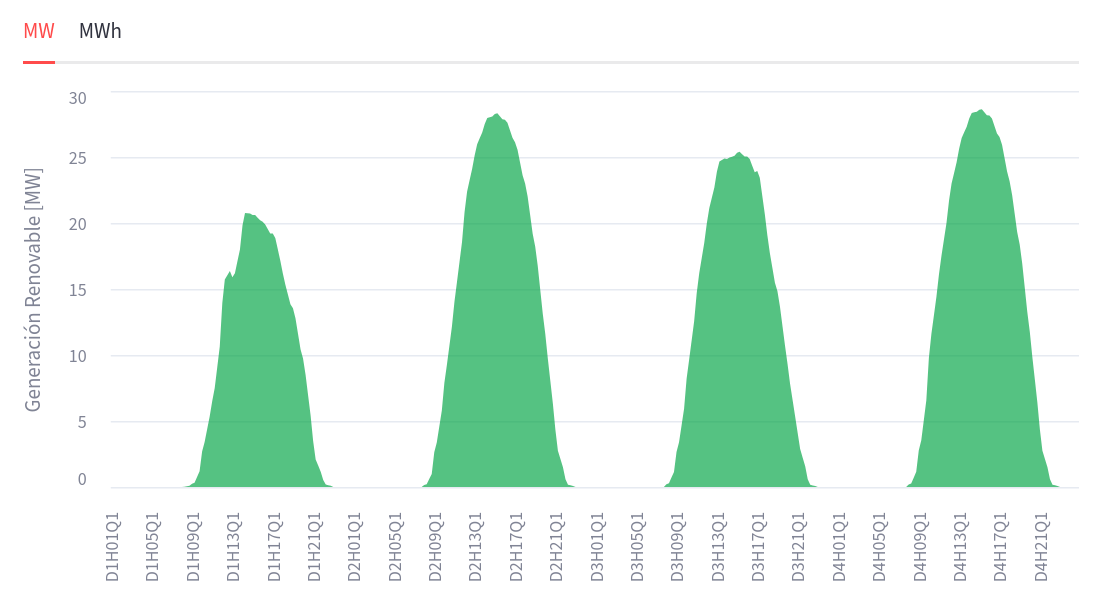
\includegraphics[width=0.75\linewidth]{figures/prevision-generacion.png}
  \caption[Previsión de generación de un activo.]{Resultado de la previsión de generación de un activo fotovoltaico.}%
  \label{fig:prevision-generacion}
\end{figure}

El sistema de optimización consume esta previsión de generación como un dato de entrada más. Las previsiones de generación permiten al sistema tener en cuenta tres aspectos fundamentales para el funcionamiento homogéneo de la instalación al completo.

\begin{itemize}

  \item Determinar los periodos en los que habrá un excedente de energía de generación que pueda ser almacenado en la batería.

  \item Evaluar el coste de oportunidad de almacenar esa energía frente a venderla directamente al mercado.

  \item Planificar la carga de la batería para maximizar el aprovechamiento de la energía generada, evitando así los peajes y cargos asociados a la carga desde la red eléctrica pública.

\end{itemize}

Por tanto, aunque el cálculo de la previsión es ajeno, su consumo es una parte relevante de la lógica del sistema, permitiendo aprovechar el potencial de las instalaciones con configuración topológica híbrida.

\section{Consolidación de información}%
\label{makereference4.4}

Una vez identificadas las fuentes de datos de mercado (\gls{omie} y \gls{ree} en este caso), el desafío fundamental reside en la adquisición programática, el procesamiento y la unificación de esta información para que pueda ser consumida por el sistema de optimización.

De esta forma, la contribución principal del sistema desarrollado en este ámbito es el diseño y la implementación de las herramientas que actúan como el puente entre estas fuentes de datos heterogéneas y la lógica de negocio, de forma paralela a las fases de extracción y transformación de un \textit{pipeline} de datos \gls{etl}.

Por lo tanto, la arquitectura elegida para esta integración es desacoplada. Los programas desarrollados se encargan de obtener los ficheros brutos, procesarlos y generar ficheros CSV estandarizados que se depositan en una ruta de intercambio de ficheros. Posteriormente, un programa externo y preexistente, ajeno a este desarrollo y equivalente a una herramienta de integración de datos como Talend~\cite{talend2025modern}, monitoriza los eventos de escritura en dicha ruta y es el responsable de ejecutar la carga final de los datos en el \gls{dw} utilizado, basado en tecnología Oracle.

Desde la perspectiva del sistema desarrollado, la fuente de datos meteorológicos es la única ya disponible directamente en la base de datos, a diferencia de la información resultante proveniente del operador del mercado y del operador del sistema que debe ser introducida en ella.

Esta arquitectura resulta ser un requisito para integrarse con herramientas internas ya existentes y, como ventaja adicional, proporciona una gran robustez frente a incidencias por parte de las fuentes de datos.

Se han desarrollado dos programas principales en Python, uno para cada fuente de datos, que se ejecutan de forma periódica según los horarios de publicación de los ficheros de cada mercado con respecto al el cierre de los mismos, si es aplicable, representado en la figura~\ref{fig:horarios-publicacion}.

\begin{figure}
  \centering
  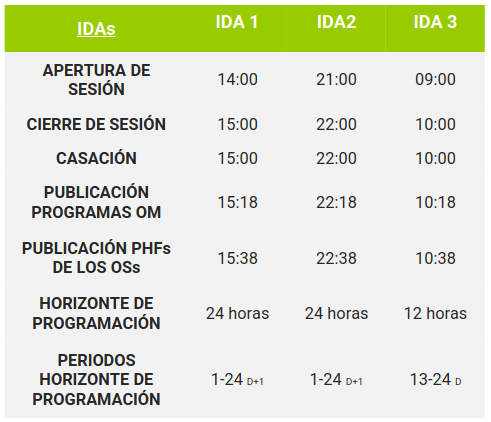
\includegraphics[width=0.5\linewidth]{figures/horarios-publicacion.png}
  \caption[Horarios de publicación de mercados intradiarios.]{Horarios de publicación de los mercados intradiarios.}%
  \label{fig:horarios-publicacion}
\end{figure}

La adquisición de datos de \gls{omie}, aunque dispone de una interfaz web, no es apta para una integración automatizada. Por ello, la comunicación se realiza a través del servidor FTP que \gls{omie} proporciona a los agentes de mercado registrados, ya que la \gls{api} que la web pública~\cite{omie2025acceso} usa no ofrece los datos en tiempo real debido a un periodo de confidencialidad.

El programa utiliza la biblioteca Paramiko\footnote{\url{https://github.com/paramiko/paramiko} (LGPL-2.1)} para establecer una conexión segura mediante SFTP con usuario y contraseña. Una vez conectado, el programa implementa una lógica para asegurar que siempre se obtiene la versión más reciente de cada fichero.

\Gls{omie} utiliza la nomenclatura \texttt{xxxxx\_aaaammdd[ss].v}, donde \texttt{xxxxx} es el nombre del fichero, \texttt{aaaa} es el año, \texttt{mm} es el mes, \texttt{dd} es el día y \texttt{ss} es la sesión del mercado, si es aplicable, y \texttt{v} es la versión del fichero.

Como se incluye una versión al final, el programa debe listar los ficheros para una fecha concreta, procesar los nombres para identificar las versiones y descargar únicamente la más alta, ya que \gls{omie} puede publicar correcciones o actualizaciones.

Para obtener las limitaciones de programa de \gls{ree}, el enfoque es similar. Se debe utilizar la \gls{api} privada de ESIOS\footnote{\url{https://participa.esios.ree.es}}, exclusiva para agentes de mercado~\cite{red2025esios}, pues la \gls{api} pública tan solo proporciona la información tras un periodo de confidencialidad. La comunicación se realiza mediante peticiones HTTP a través de la biblioteca Requests\footnote{\url{https://github.com/psf/requests} (Apache-2.0)}, utilizando autenticación OAuth con un token de acceso tipo \textit{bearer}.

Una vez obtenidos los ficheros, que se presentan en formatos CSV específicos, la biblioteca Pandas\footnote{\url{https://github.com/pandas-dev/pandas} (BSD-3-Clause)} se encarga de la transformación. El resultado es un fichero CSV cuyo formato se corresponde directamente con las filas a insertar en la base de datos de destino.

El formato de los datos de precios contiene las columnas fecha, hora y precio en euros por megavatio hora\footnote{Es importante destacar que el campo de hora representa el periodo de mercado, porque anteriormente la granularidad de los mercados era exclusivamente horaria.}, según la tabla~\ref{tab:descripción-precio} y el contenido de la figura~\ref{fig:contenido-precio}.

\begin{table}[ht]
  \centering
  \begin{tabular}{|l|p{7.5cm}|l|}
    \hline
    Campo      & Descripción                     & Valores válidos            \\
    \hline
    Año        & Año                             & I4 {-}{-} 20XX             \\
    Mes        & Mes                             & I2 {-}{-} 1 a 12           \\
    Día        & Día                             & I2 {-}{-} 1 a 31           \\
    Hora       & Hora                            & I2 {-}{-} 1 a 25           \\
    MarginalPT & Precio marginal zona Portuguesa & F8.2 {-}{-} 0.0 a 99999.99 \\
    MarginalES & Precio marginal zona Española   & F8.2 {-}{-} 0.0 a 99999.99 \\
    \hline
  \end{tabular}
  \caption[Descripción del formato de precios.]{Descripción del formato de precios~\cite{omie2025modelo}.}%
  \label{tab:descripción-precio}
\end{table}

\begin{figure}
  \centering
  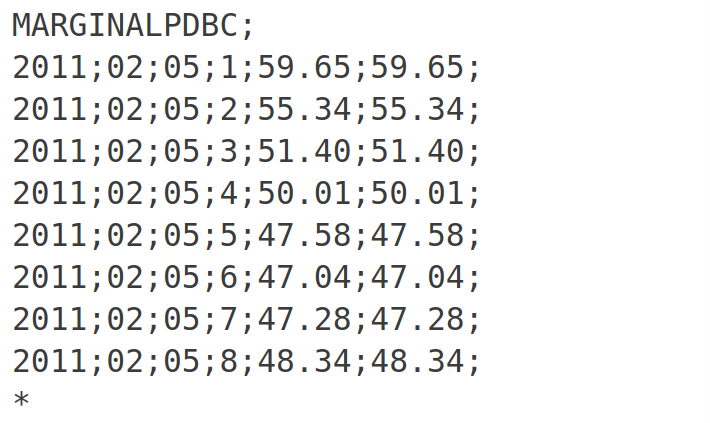
\includegraphics[width=0.5\linewidth]{figures/contenido-precio.png}
  \caption[Ejemplificación del contenido de los ficheros de precio.]{Ejemplificación del contenido de los ficheros de precio.}%
  \label{fig:contenido-precio}
\end{figure}

El desarrollo gestiona correctamente los husos horarios en horario local, ya que el mercado diario dispone de 24 periodos de granularidad horaria, pero puede tener 23 o 25 en días con cambio de hora\footnote{El mercado diario está en proceso de ser actualizado a una granularidad cuartohoraria.}. Análogamente, los mercados intradiarios, con granularidad cuartohoraria, tienen por lo general 96 periodos, con opción de 92 y 100. Esto es debido a que el funcionamiento de los mercados siempre se realiza en horario local, sin excepción, para que no existan conflictos de solapamiento entre ellos~\cite{omie2025reglas}.

El fichero de energía negociada contiene las columnas UP, fecha, hora y energía en megavatios hora. De esta forma, la presencia de la \gls{up} es la razón fundamental del carácter confidencial de estos datos. Si un agente conociera los movimientos de las unidades que no controla, podría adaptar su estrategia en detrimento de la libre competencia, según la tabla~\ref{tab:descripción-energia} y el contenido de la figura~\ref{fig:contenido-energia}.

\begin{table}[ht]
  \centering
  \begin{tabular}{|l|p{5cm}|l|}
    \hline
    Campo             & Descripción                                                                                       & Valores válidos                \\
    \hline
    Año               & Año                                                                                               & I4 {-}{-} 20XX                 \\
    Mes               & Mes                                                                                               & I2 {-}{-} 1 a 12               \\
    Día               & Día                                                                                               & I2 {-}{-} 1 a 31               \\
    Hora              & Hora                                                                                              & I2 {-}{-} 1 a 25               \\
    Código            & Código de la unidad (UP) ofertante                                                                & A7                             \\
    Energía asignada  & Energía asignada (MWh)                                                                            & F7.1 {-}{-} -99999.9 a 99999.9 \\
    IdCBF             & Identificador del Cont. Bilateral                                                                 & I8 Vacío cuando es una oferta  \\
    Tipo de oferta    & Indicará que tipo de oferta es                                                                    & I2 {-}{-} 0 a 99               \\
    NumOf             & Indicará el número de oferta ó el de ejecución del contrato bilateral físico asociado a la unidad & I8 {-}{-} -1 a 99999999        \\
    \hline
  \end{tabular}
  \caption[Descripción del formato de energía negociada.]{Descripción del formato de energía negociada~\cite{omie2025modelo}.}%
  \label{tab:descripción-energia}
\end{table}

\begin{figure}
  \centering
  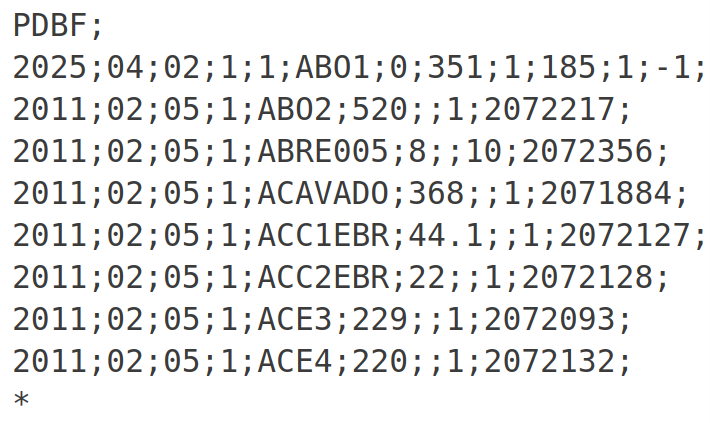
\includegraphics[width=0.5\linewidth]{figures/contenido-energia.png}
  \caption[Ejemplificación del contenido de los ficheros de energía.]{Ejemplificación del contenido de los ficheros de energía.}%
  \label{fig:contenido-energia}
\end{figure}

Aún con todo, existe un enorme problema que impide el uso de los resultados de la energía casada de forma directa. Esto se debe a que el sistema desarrollado necesita la información de la energía casada no por \gls{up}, sino por \gls{ufi}, de tal forma que se pueda arbitrar de forma independiente.

Para resolver este problema, se hace uso de una herramienta propietaria externa al desarrollo, que es capaz de calcular los desgloses de la energía, convirtiendo la energía casada por \gls{up} a energía casada por \gls{ufi}. Para llevarlo a cabo, debe hacer uso de información no disponible por el desarrollo, por lo que la existencia de una herramienta del estilo es necesaria.

Junto a ello, el fichero de limitaciones de programa se estructura con las columnas fecha, hora, \gls{up}, \gls{ufi} y valor, según el contenido de la figura~\ref{fig:contenido-limitaciones}. La lógica es que si el código es un \gls{ufi}, la limitación aplica exclusivamente a ese activo físico, si es un \gls{up}, se aplica a la totalidad de la instalación.

\begin{figure}
  \centering
  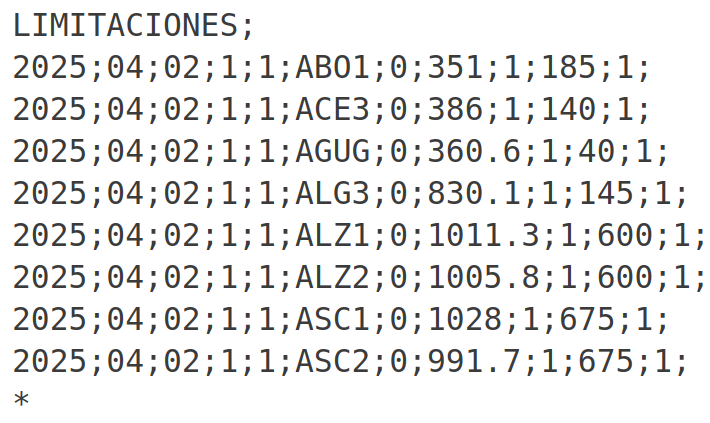
\includegraphics[width=0.5\linewidth]{figures/contenido-limitaciones.png}
  \caption[Limitaciones de programa a una instalación.]{Limitaciones de programa a una instalación.}%
  \label{fig:contenido-limitaciones}
\end{figure}

Todos estos archivos son transformados al formato interno de inserción y entregados al intercambiador de ficheros.

Una vez los datos residen en el \gls{dw}, el sistema de optimización los consume mediante consultas SQL\@. Sin embargo, una simple consulta no es suficiente, ya que las inserciones en la base de datos están sujetas a un versionado interno, independiente del versionado de los ficheros de origen.

Por esta razón, es necesario utilizar consultas analíticas de SQL que, específicamente, empleen funciones de ventana particionadas por la fecha y los periodos de mercado, y las \gls{up} o \gls{ufi}, si es aplicable. De este modo, se ordenan según la versión interna para garantizar que siempre se seleccione la versión más reciente de la información.

Además, se han realizado esfuerzos extensivos para reducir significativamente la latencia de estas consultas, un factor crítico para disminuir el tiempo de respuesta del sistema al completo.

El enfoque del sistema desarrollado consiste en construir consultas que filtran de manera agresiva sobre las columnas indexadas de las tablas base, asegurando que el motor de Oracle utilice planes de ejecución altamente eficientes.

Esta arquitectura desacoplada también facilita la gestión de incidencias, como se ha mencionado anteriormente. En ocasiones, \gls{omie} o \gls{ree} no publican los ficheros a tiempo. En estos casos, el proceso requiere una intervención manual en la que el agente de mercado responsable contacte con la institución correspondiente, y que esta llegue a enviar el fichero ausente por un canal alternativo, como correo electrónico.

Gracias al diseño, el operador puede procesar este fichero manualmente con los programas desarrollados y depositar el resultado en la ruta de intercambio, permitiendo que el flujo de datos se complete sin alterar el proceso de carga.

% \cleardoublepage

\chapter{Modelización estructural}
\label{makereference5}

Una vez obtenidos tanto los datos de las señales de la infraestructura operacional y la información del entorno del mercado, es necesario realizar un modelado estructural del entrono a optimizar para, tomadas las entradas, determinar la posición del mercado óptima de las baterías.

Exactamente, el objetivo principal de la etapa de optimización del sistema es responder a las cuestiones de cuándo y de qué fuente ciclar energía y cuánta energía ciclar, buscando siempre los mayores ingresos.

Para ello, se ha elegido pyomo como herramienta de modelización matemática en el área de investigación operacional. Pyomo es una librería de Python para formular, solucionar y analizar problemas de optimización como el presente.

Se hace uso de una formulación de programación lineal de enteros mixtos para poder tener en cuenta condiciones más allá de la más simple programación lineal. Se ha explorado el uso de indicadores o restricciones avanzadas, como los \textit{special order sets}, los cuales han sido descartados en última instancia debido a problemas de rendimiento. Esto significa que la modelización es puramente de enteros mixtos compatible con cualquier solucionador que soporte variables binarias.

De esta forma, se detallan los parámetros de decisión en la sección~\ref{makereference5.1}, que articulan el problema de optimización, abarcando desde la definición temporal de los periodos del mercado y las variables de operación de los flujos energéticos, hasta las limitaciones impuestas por el comportamiento físico de la batería y las guías estratégicas de las indicaciones de mercado. Se procede a formular las restricciones operacionales que aseguran la viabilidad técnica de la solución en la sección~\ref{makereference5.2}, se habla de la optimización dual de la instalación al completo de la generación energética en la sección~\ref{makereference5.3}, se establece el criterio de desempeño que define la función objetivo a optimizar en la parte~\ref{makereference5.4} y, finalmente, se consideran los requisitos de la resolución numérica para cumplir con la precisión exigida por el operador del mercado en la sección~\ref{makereference5.5}.

\section{Parámetros de decisión}
\label{makereference5.1}

Todo modelado estructural debe contar inicialmente con un conjunto de parámetros de decisión que determinen los valores con los que trabaja el modelo. Más adelante, dichos parámetros son usados para definir las restricciones que el control de la batería debe cumplir.

\subsection{Periodos del mercado}
\label{makereference5.1.1}

El mercado eléctrico peninsular opera en etapas discreta temporales con una granularidad establecida. Los mercados spot, de los que se encarga el sistema en la actualidad, disponen de una granularidad horaria para el mercado diario\footnote{La granularidad del mercado diario se encuentra en proceso de actualización a cuarto horaria} y cuarto horaria para los mercados intradiarios, tanto europeos como las sesiones del continuo. En el resto de mercados de Europa, como Nord Pool, la granularidad de los mercados spot es similar, existiendo también granularidades incluso de 30 minutos.

La variabilidad de la granularidad exige representar el mercado en múltiples periodos categóricos de tamaña proporcional a ella. De esta forma, el sistema dispone por un lado de una granularidad configurable \( \Delta t \), llamada oficialmente unidad de tiempo de mercado, y el set que representa mercado mismo~\ref{eq:set-mercado}.

\begin{equation}
  \label{eq:set-mercado}
\end{equation}

Es necesario tener en cuenta los usos horarios a la hora de calcular el tamaño del mercado, ya que los mercados siempre y en todo momento hacen uso del uso horario local, a diferencia de UTC. Esto significa que en los día de cambio de hora, los mercados del día tendrán más o menos periodos y el mercado intradiario continuo tendrá más o menos sesiones, dependiendo de si se añaden o restan horas. El operador del mercado lo detalla en la tabla~\ref{tab:cambio-hora}.

\begin{table}[ht]
  \centering
  \begin{tabular}[c]{|l|l|l|}
    \hline
    Código & Descripción & Tipo de producción \\
    \hline
    \hline
  \end{tabular}
  \caption{Ajustes del mercado en cambios de hora}
  \label{tab:cambio-hora}
\end{table}

La representación del mercado durante la optimización realmente incluye multiples posibles mercados futuros más allá del más proximo, es decir, el sistema tiene en cuenta un horizonte de optimización de varios mercados y, por lo tanto, varios periodos a lo largo de múltiples días de mercado. La razón de lo cual reside en facilitar la mayor información posible: si un día de mercado no cumple con las condiciones de actuación mientras que otro día de mercado las dobla, es posible no arbitrar uno de los días y ofertar el doble el otro, en vez de perder la oportunidad, representado en la figura~\ref{fig:horizonte-de-optimizacióno}.

\begin{figure}
  \centering
  \includegraphics[width=0.5\linewidth]{figures/horizonte-de-optimizacióno.jpg}
  \caption{Representación del horizonte de optimización}
  \label{fig:horizonte-de-optimizacióno}
\end{figure}

\subsection{Flujos energéticos}
\label{makereference5.1.2}

El mercado, precisamente, es usado para indexar los flujos energéticos explicados en la sección~\ref{makereference3.1} de infraestructura operacional. Estos flujos energéticos representan la operación y, por lo tanto, salida de la optimización. Responden a las tres preguntas planteadas anteriormente.

La configuración topológica más simple, la configuración topológica aislada, tan solo dispone de dos: el flujo de importación de la red al sistema de almacenamiento de energía en baterías y exportación del sistema de almacenamiento de energía en baterías a la red. La configuración topológica añade uno más, la importación de la generación al sistema de almacenamiento de energía en baterías.

Aún así, ellos solos no bastan para controlar la batería correctamente. Para ello, conviene más observar estos flujos energéticos no como flujos energéticos mismos, sino como interfaces de compra y venta, como las unidades físicas explicadas en el apartado~\ref{makereference4}. Realmente, el sistema se encarga de arbitrar en el mercado, por lo que debe operar no solo en la capa de abstracción de flujos energéticos físicos, sino además en la de los movimientos del mercado.

Todo esto es para subrayar que los flujos energéticos, desde la perspectiva del mercado, no están limitados a únicamente a la dirección de compra para la carga y venta para la descarga. Una unidad física correspondiente a la importación de energía es capaz de venderla también, solo que esa energía vendida no puede provenir de la instalación perteneciente a la unidad física, ya que el flujo energético fisco limita la venta.

Por ejemplo, como se realizan varias sesiones de mercado en un mismo día, puede que el sistema haya prometido vender una cantidad de energía en un periodo de la tarde en el mercado diario. Lamentablemente, una hora antes de tener que exportar toda esa energía casada (en la última sesión del mercado intradiario continuo antes del \textit{delivery}), resulta que las nuevas previsiones meteorológicas indica que, debido a una nube repentina, los paneles fotovoltaicos no van a ser capaces de generar la suficiente energía como para cargar la batería y exportar su energía. Esto genera un desvío en la posición de la batería: no va a ser capaz de otorgar toda la energía prometida y puede resultar penalizada. Por suerte, como se ha explicado, la solución al problema es recomprar la cantidad de energía que le falte al sistema a través de la interfaz de exportación. Como las recompras (y reventas, en el caso contrario) se realizan exclusivamente en el mismo periodo de su correspondiente posición opuesta por definición, la energía no necesita pasar por la interfaz que ha realizado la operación y la instalación puede exportar la energía tranquilamente y suplir la falta al mismo tiempo, sin tener que importan energía a la instalación.

Por lo tanto, los diferentes flujos energéticos son representados de la siguiente forma, correspondientes con los resultados principales de la optimización

...

\subsection{Comportamiento físico}
\label{makereference5.1.3}

Aunque los anteriores flujos energéticos sean dependientes de la configuración topológica, toda batería comparte unos comportamientos físicos intrinsecos. Al fin y al cabo, las baterías son sistemas de almacenamiento de energía que permiten ser cargadas para su posterior descarga, pero ¿cómo de rápido pueden ser cargadas y descargadas, cuánto, cuántas veces, etc.?

Precisamente, las señales configuradas propiamente en el sistema de información de planta detalladas en la sección~\ref{makereference3.2} permite conocer los parámetros operacionales de las batería. Con ellos, lo que es necesario es representarlos por el sistema para su optimización operativa.

...

\subsection{Indicaciones de mercado}
\label{makereference5.1.4}

Finalmente, los previos parámetros completan la modelización de la batería, en cambio, el sistema debe ser capaz de guiar la operación de la batería. Es decir, impedir situaciones posibles físicamente realizables por la batería pero que no interesan.

Para ello, el sistema define el ingreso obtenido y los ciclos realizados como los principales indicadores de rendimiento, por lo tanto, se expresan los siguientes parámetros que los controlan.

...

\section{Restricciones operacionales}
\label{makereference5.2}

Conociendo los parámetros con los que trabaja el apartado de optimización del sistema, es momento de definir las restricciones operacionales que establecen las relaciones entre ellos. Las ecuaciones mostradas se encuentran simplificadas para facilitar la comprensión aunque resulten más robustas en la realidad. No se muestran, por ejemplo, las restricciones de consignación manual tanto de la posición como el estado de carga, explicadas en el apartado~\ref{makereference6}.

Como algunas configuraciones topológicas no soportan todos los flujos energéticos, como la importación de la red en la híbrida con carga aislada de la red o la importación de la generación en la aislada, estas deben ser capaces de ser desactivadas a través de la simple formula~\ref{eq:desactivación-ufi}.

\begin{equation}
  \label{eq:desactivación-ufi}
\end{equation}

Con esto, los flujos energéticos netos están definidos como la suma del correspondiente flujo energético bruto y el casado, es decir, el flujo energético físico representado por el parámetro neto debe ser siempre no negativo, pero la interfaz de la unidad física lo puede ser cuando existan posiciones casadas en un periodo concreto. Esto es representado por la ecuación~\ref{eq:neto-bruto} y se realiza para cada uno de los flujos energéticos con unidades físicas arbitrados en el mercado, es decir, la importación de la red y la exportación a la red.

\begin{equation}
  \label{eq:neto-bruto}
\end{equation}

Con respecto a los parámetros del comportamiento físico, estos limitan la potencia tanto de carga como de descarga\footnote{Aunque la potencia de carga y descarga generalmente coincida en las instalaciones para las que se ha desplegado el sistema, es importante reconocer que pueden no ser iguales} mediante la ecuación~\ref{eq:capacidad-potencia-carga} de carga y la ecuación~\ref{eq:capacidad-potencia-descarga} de descarga. La señal de disponibilidad afecta linealmente a la capacidad de potencia, para una disponibilidad de la mitad, la potencia de la batería es la mitad misma de su capacidad nominal.

\begin{equation}
  \label{eq:capacidad-potencia-carga}
\end{equation}

\begin{equation}
  \label{eq:capacidad-potencia-descarga}
\end{equation}

Y junto a la potencia, la capacidad de almacenamiento la limita el correspondiente parámetro nominal de la batería en~\ref{eq:capacidad-almacenamiento}.

\begin{equation}
  \label{eq:capacidad-almacenamiento}
\end{equation}

Las eficiencias de carga y descarga también afectan al ciclado. Precisamente, es absolutamente necesario separar la carga por un lado y la descarga por otro ya que una de los indicadores de rendimiento es el número de ciclos. Como se indica oficialmente: "se completa un ciclo de carga cuando se ha usado (descargado) una cantidad equivalente al 100 \% de la capacidad de la batería, pero no necesariamente toda con una sola carga. Por ejemplo, podrías usar el 75 \% de la capacidad de la batería un día y luego recargarla completamente durante la noche. Si usas el 25 \% al día siguiente, habrás descargado el 100 \% en total, y los dos días sumarán un ciclo de carga."

Esto significa que si la carga y la descarga no se separase, el número de ciclos sería contado incorrectamente ya que podrían realizarse ciclos que dejasen la batería en el mismo estado, y seguir siendo ciclos perfectamente válidos. De esta forma, las ecuaciones de las eficiencias detallan la carga proveniente tanto de la importación de la red y de la importación de la generación en~\ref{eq:eficiencia-carga} y la descarga en~\ref{eq:eficiencia-descarga}.

\begin{equation}
  \label{eq:eficiencia-carga}
\end{equation}

\begin{equation}
  \label{eq:eficiencia-descarga}
\end{equation}

Aún así, separar la carga y la descarga introduce uno de los mayores problemas del sistema, la carga y descarga simultanea. La defensa ante esta situación, invalida físicamente debido al funcionamiento de la conexión interna de las baterías, es realizada para la consignación en la sección~\ref{makereference6.1.1}. Durante la optimización, en cambio, se tiene en cuenta usando la programación de enteros mixtos previamente mencionada y sus pertinentes variables binarias en la formulación~\ref{eq:carga-descarga-simultánea}.

\begin{equation}
  \label{eq:carga-descarga-simultánea}
\end{equation}

Un aspecto a tener en cuenta es que la formulación puede realizarse usando \textit{special order sets} para evitar el uso de variables Big M, como se indica en la ecuación~\ref{eq:carga-descarga-simultánea-sos}. Si las variables de carga y descarga (y el resto más adelante) no estuvieran limitadas físicamente (Big M arbitrariamente alto), esto podría afectar negativamente al rendimiento del sistema, pero como sí lo están, no existen problemas de estabilidad numérica.

\begin{equation}
  \label{eq:carga-descarga-simultánea-sos}
\end{equation}

El indicador de mercado de ciclos máximos limita simplemente los ciclos mediante la ecuación~\ref{eq:limite-ciclos}. Para no introducir relaciones no lineales y afectar negativamente al rendimiento del sistema, el indicador de mercado de ciclos máximos proviene de la verdadera opción de configuración expuesta a los agentes de mercado y operadores de telecontrol en forma de ciclos máximos por día y multiplico directamente por el número de días del horizonte de optimización \( ... \). Aunque esto conlleva que los ciclos puedan repartirse a lo largo del horizonte de optimización, a diferencia de una solución no lineal, no es ningún problema, verdaderamente.

\begin{equation}
  \label{eq:limite-ciclos}
\end{equation}

El estado de carga lo limitan las señales de la batería en la ecuación~\ref{eq:limite-soc}. Generalmente, se suele dejar una cantidad de energía disponible continuamente para evitar imprevistos.

Precisamente, un efecto secundaria inmensamente beneficioso de las limitaciones de la señal del estado de carga es la posibilidad de la participación de las baterías en los mercados de disponibilidad\footnote{El sistema no soporta los mercados de disponibilidad en su estado actual, aunque sí que permite manejarlos externamente}. Como en ningún momento se llega ni al máximo ni al mínimo de la capacidad de la batería, esta puede ofertar por lo menos el rango del estado de carga a subir o bajar y generar beneficios pasivos sin afectar de ninguna forma a la operación principal en los mercados spot.

\begin{equation}
  \label{eq:limite-soc}
\end{equation}

Continuando con el estado de carga, es necesario conocer por lo menos el estado de carga inicial de donde se parte, ecuación~\ref{eq:soc-inicial}, y también determinar asignar el estado de carga final, ecuación~\ref{eq:soc-final}, para ejecutar grupos de ciclado consistentes en donde el estado de carga de la batería no termine en un valor indeterminado.

\begin{equation}
  \label{eq:soc-inicial}
\end{equation}

\begin{equation}
  \label{eq:soc-final}
\end{equation}

De esta forma, se define la ecuación del estado de carga~\ref{eq:soc}, teniendo en cuenta la energía cargada y descargada.

\begin{equation}
  \label{eq:soc}
\end{equation}

Ademas, la modelización también debe tener en cuenta las limitaciones de programa obtenidas en la sección~\ref{makereference4.2.1}. Estas limitaciones impiden la exportación de energía de cada uno de los activos energéticos individualmente.

...

Esta nueva restricción, en cambio, introduce nuevas oportunidades de arbitraje ya que las limitaciones no son de la instalación al completo (también), sino individuales según el activo energético. Esto significa que puede que la generación se vea limitada (el funcionamiento de la misma es explicado en la sección~\ref{makereference5.3}) pero no la exportación de la batería. Ante dicha situación, la batería es capaz de cargarse sin ningún coste.

Para tener mejorar el rendimiento y tener en cuenta esos escenario, se introducen nuevas restricciones en forma de la ecuación~\ref{eq:curtailed-import}, que controla la importación de energía excedente, y la ecuación~\ref{eq:uncurtailed-import}, que controla la importación de energía no excedente. De hecho, el termino usado para referirse a la energía excedente se conoce como \textit{curtailment}.

\begin{equation}
  \label{eq:curtailed-import}
\end{equation}

\begin{equation}
  \label{eq:uncurtailed-import}
\end{equation}

Estas nuevas restricciones, lamentablemente, introducen otro nuevo conflicto. ¿Cómo se decide si cargar de la energía excedente o de la no excedente? Entendiblemente, siempre es necesario priorizar la carga de la energía excedente, por lo que se añade otra indicación de enteros mixtos a la formulación, ecuación~\ref{eq:indicador-curtailment}. De la mismo forma que el Big M anterior, la importación tanto excedente como no excedente cuenta con un límite superior en forma de la cantidad de energía disponible, por lo que no existen problemas de estabilidad numérica directos.

\begin{equation}
  \label{eq:indicador-curtailment}
\end{equation}

Para terminar con lo relacionado con los sistemas de almacenamiento de energía en baterías mismos, por el momento solo se ha tenido en cuenta una configuración topológica del estilo de la aislada e híbrida flexible, ya que, según se ha descrito hasta ahora, el sistema puede importar energía de la red o de la generación libremente (bajo el resto de restricciones).

En cambio, no todas las configuraciones topológicas operan de la siguiente manera. Precisamente, la híbrida con carga aislada de la red muestra un comportamiento de \textit{clipping}, en donde existe una cantidad de energía excedente de donde la batería solo puede cargar.

Representado en la figura~\ref{fig:clipping}, se puede entender como una persona que dispone de un salario fijo (generación). Cada mes debe pagar una cantidad de su salario para el alquiler (\textit{threshold} de carga). Del dinero sobrante, ahorra (carga) una porcentaje (coeficiente de \textit{clipping}), mientras que gasta el resto como le apetezca (exportación de generación).

\begin{figure}
  \centering
  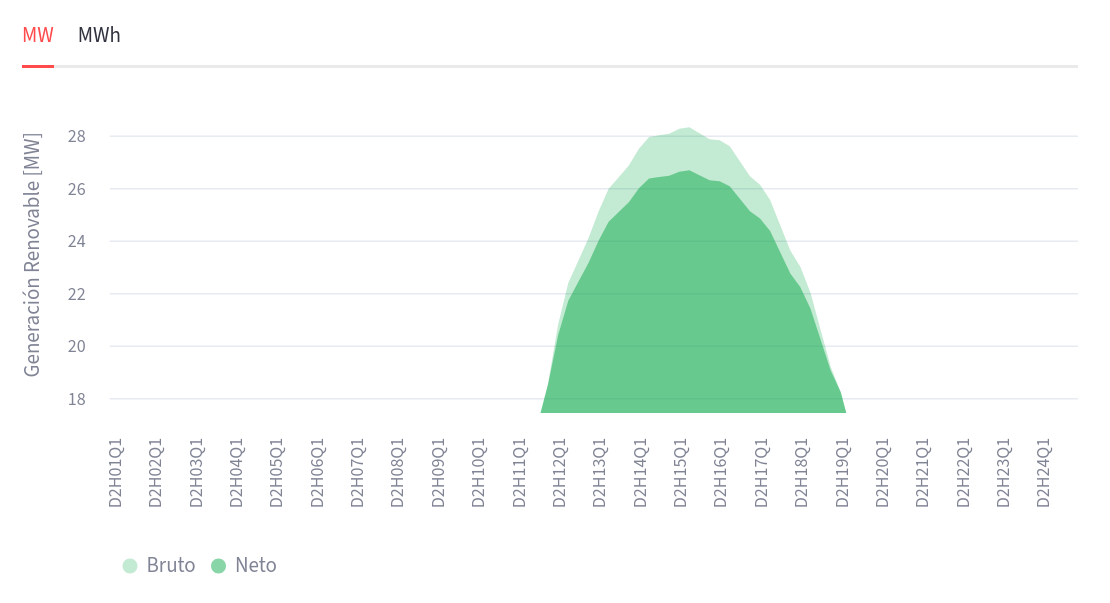
\includegraphics[width=0.5\linewidth]{figures/clipping.jpg}
  \caption{Clipping de la configuración topológica híbrida con carga aislada de la red}
  \label{fig:clipping}
\end{figure}

El sistema lo representa mediante la ecuación~\ref{eq:clipping}.

\begin{equation}
  \label{eq:clipping}
\end{equation}

La última configuración topológica a tener en cuenta se trata de la híbrida con prioridad de carga de generación. Esto significa que se debe agotar completamente el recurso de generación antes de poder cargar de la red, aunque cargar de la red otorgue mayores beneficios, como es el caso de los precios de mercado negativos.

Dicha prioridad es definida de forma simular a previas restricciones de indicación Big M con enteros mixtos en la ecuación~\ref{eq:prioridad-híbrida}.

\begin{equation}
  \label{eq:prioridad-híbrida}
\end{equation}

Como se puede observar, el sistema es completamente genérico e incorpora comportamientos, a diferencia de definir entidades separadas para cada configuración. Es decir, el sistema usado es exactamente el mismo para cualquier configuración.

\section{Generación energética}
\label{makereference5.3}

Aunque, la modelización anterior cubra el comportamiento de los sistemas de almacenamiento de energía en baterías al completo, al sistema le surge un pequeño problema, ¿cómo decide cuándo cargar de la red o de la generación?

Las restricciones previas tan solo dibujan un marco general pero no tienen en cuenta que la energía importada de la generación es energía que la instalación, a través de la interfaz de exportación de la generación, no es capaz de vender, la carga de la batería lo impide.

Por lo tanto, es necesario tener en cuenta la generación junto con la batería y realizar una optimización de los flujos energéticos de la instalación al completo, incluida la generación. Si añadimos la generación al criterio de desempeño de la sección~\ref{makereference5.4}, la batería no podrá "robar" energía a la generación ya que debe existir una armonía conjunta en busca de la maximización del ingreso.

Precisamente y como se ha afirmado anteriormente, uno de los propósitos principales del sistema es su uso avanzado en instalaciones híbridas, como se puede observar.

...

\section{Criterio de desempeño}
\label{makereference5.4}

Como se ha mencionado en múltiples ocasiones, el criterio de desempeño del sistema parece ser el beneficio obtenido, es decir, el sistema busca maximizar los ingresos, en cambio, esto no es del todo cierto.

En el beneficio toma parte cada flujo de energía. Importantemente, como el sistema asume que las recompras y reventas se realizan al mismo precio que la posible compra y venta, tan solo se tienen en cuenta los flujos energéticos netos, correspondientes a los flujos físicos, para las interfaces de mercado. Con ello, se le asigna un precio a cada uno de ellos, resultando en la ecuación~\ref{eq:beneficio}.

\begin{equation}
  \label{eq:beneficio}
\end{equation}

Si bien la maximización del beneficio es uno de los objetivos, el principal precisamente, el sistema debe tener en cuenta otros factores. De hecho, cuando se realiza la optimización, tener en cuenta el beneficio unicamente resulta, casi con total certeza, en un problema de optimización degenerado.

Los problemas de optimización degenerados son los que poseen múltiples soluciones para una misma formulación. El sistema, por el contrario, debe asegurar una optimización determinista (llamada estricta) para facilitar el control de las baterías, no se puede permitir que ante cualquier modificación en su configuración, por muy minúsculo que sea, la posición óptica cambie drásticamente y genere desvíos. La diferencia se observa en la figura~\ref{fig:degenerada-vs-estricta}.

\begin{figure}
  \centering
  \includegraphics[width=0.5\linewidth]{figures/degenerada-vs-estricta.jpg}
  \caption{Comparación entre una posición degenerada y su contraparte estricta}
  \label{fig:degenerada-vs-estricta}
\end{figure}

Para solucionar este problema, se tiene en cuenta que las predicciones de precio de mercado y las predicciones meteorológicas, es decir, la información extraída en el apartado~\ref{makereference4} del entorno de mercado, es más precisa cuanto más cercana en el tiempo sea. En otras palabras, las previsiones para el día de mañana resultan más fiables que las de dentro de 5 días.

Dentro de la formulación, esta preferencia de las posiciones más cercanas en el tiempo se representa con una función de decrecimiento o \textit{decay function} exponencial, ecuación~\ref{eq:exponential-decay}. Dispone de un ratio de decrecimiento configurable dependiente del horizonte de optimización, cuanto mayor sea menor valor tendrá el ratio de decrecimiento, para evitar conflictos en donde peor posición más cercana en el tiempo sea elegido ante una mejor más lejana.

\begin{equation}
  \label{eq:exponential-decay}
\end{equation}

De esta forma, tras realizar el llamado test de factibilidad básica e identificar las variables básicas\footnote{Las variables básicas son las que marcan los puntos extremos de las soluciones, pero no tienen por que encontrarse en su límite, lo cual resultó ser fuente de confusión en el análisis de factibilidad} y sus propiedades, se determina la estrictez de la formulación.

\section{Optimización lexicográfica}
\label{makereference5.4.1}

Aunque el uso de una función de decrecimiento incorpore distinga correctamente las soluciones de forma determinista, técnicamente es posible, dependiendo de los parámetros de configuración, que la solución obtenida por el solucionador sea la óptima según el criterio de desempeño definido, pero no la que el sistema busca. Esto sucede debido a que parámetros de decisión incorrectamente seleccionados pueden priorizar una posición que mejore el objetivo de la preferencia temporal y no el del beneficio.

La metodología anterior de juntar los dos objetivos se conoce como optimización multiobjetivo ponderada, donde el coeficiente de ponderación es el calculado mediante la \textit{decay function} exponencial. Aún así, existe una técnica de optimización multiobjetivo más avanzada que evita conflictos entre ellos gracias a una metodología de priorización de objetivos, llamada optimización lexicográfica.

De esta forma, se desarrolla el algoritmo~\ref{alg:optimización-lexicográfica} de optimización lexicográfica multiobjetivo por encima del lenguaje de modelado abstracto para asegurar la priorización de los objetivos de la modelización, ya que la herramienta de modelado utilizada no soporta solucionar múltiples objetivos al mismo tiempo.

\begin{algorithm}
  \caption{Optimización lexicográfica}
  \label{alg:optimización-lexicográfica}
  \begin{algorithmic}
    \State $i \gets 10$
    \If{$i\geq 5$}
    \State $i \gets i-1$
    \Else
    \If{$i\leq 3$}
    \State $i \gets i+2$
    \EndIf
    \EndIf
  \end{algorithmic}
\end{algorithm}

Con esto, el objetivo principal se trata de la maximización del beneficio y el objetivo secundario la priorización temporal (porque se sigue necesitando obtener una única solución). El sistema permite definir otros objetivos secundarios de menor prioridad, como la maximización del estado de carga final para aprovechar situaciones de carga gratuita en las que la energía no es vendida.

Aunque se solucionen los problemas de posiciones posiblemente no óptimas, la optimización lexicográfica tiene un menor rendimiento, por lo que no es factible usarla para mercados con una granularidad muy pequeña, como los de disponibilida. En cambio, funciona adecuadamente para los mercados spot en los que se centra el despliegue realizado del sistema.

\section{Resolución numérica}
\label{makereference5.5}

Otro aspecto a tener en cuenta es la precisión numérica de los resultados. De hecho la institución regulatoria del mercado eléctrico correspondiente, el operador del mercado mismo, define las regulaciones de la precisión numérica aceptada para el arbitraje.

Tanto la energía como la potencia son expresados con una precisión de un solo decimal, siendo su granularidad una décima de megavatio y megavatio hora. El precio de oferta, en cambio, se expresa con dos decimales

Irónicamente, las minúsculas diferencias entre los resultados reales correspondientes al estado de la batería y las ofertas de arbitraje sí que son capaces de generar desvíos en el mercado. Por suerte, el sistema no tiene por que encargarse de dicha discrepancia debido a que los desvíos son comparativamente tan bajos, menores a 50 kilovatios hora (\textit{kWh}) de media, que la red eléctrica misma es capaz de absorber sin absolutamente ningún problema. Además, como los desvíos resultan tanto a subir como bajar, generalmente se contrarrestan entre sí.

\cleardoublepage

\chapter{Comando y control}
\label{makereference6}

Teniendo disponible toda la información necesaria para el control de vuelta al \gls{bess}, es necesario convertirla a la señales que la batería entiende. A su vez, también se necesita comunicar las ofertas de compra y venta de energía al mercado, para garantizar la sincronía de las operaciones entre la carga y compra y descarga y venta de la energía, respectivamente.

Más allá de las operaciones mismas, en entornos industriales donde se mueven grandes cantidades de energía, como el pertinente, es altamente recomendable disponer de algún tipo de método con el que comprobar la correcta operación del sistema y modificar su comportamiento si resulta oportuno. Por ello, también se desarrolla un cuadro de mando con el que realizar las tareas de supervisión.

De esta forma, el apartado~\ref{makereference6.1} describe la operación automática del control de las consignas de la batería y las ofertas de mercado, mientras que el apartado~\ref{makereference6.2} detalla la implementación del cuadro de mando con el que supervisar la operación del sistema.

\section{Consignación operativa}
\label{makereference6.1}

La consignación operativa no solo incluye la señalización del perfil de carga y descarga de las baterías y es que, si el sistema no comunica adecuadamente sus intenciones de compra y venta mediante los medios preestablecidos, la entidad energética dueña de la instalación podría incurrir severas multas por incumplir el reglamento.

Con ello, el sistema debe responder a las cruciales preguntas de cuándo y cuánta energía ciclar físicamente y a qué precio.

\subsection{Señalización de baterías}
\label{makereference6.1.1}

Las señales de los \gls{bess} se comunican en términos de energía, como se describe en la sección~\ref{makereference3.2}. Esto significa que a las baterías no se les pueden mandar consigas de cargar o descargar una cantidad determinada de energía por cada periodo de mercado, aunque este sea el formato de salida de la optimización. Precisamente, la razón de esta limitación es bastante sencilla, la energía es dependiente del tiempo. La potencia, en cambio, es instantánea.

Resulta que, al igual que todo el resto de activos energéticos, la operación de los \gls{bess} es medida en potencia, representando el ritmo con el cual la batería transfiere energía.

Dependiendo de la posición de arbitraje, la batería puede encontrarse a diferentes perfiles de potencia, desde la inactividad y el llamado mínimo técnico, hasta el máximo operacional. En la figura~\ref{fig:perfil-potencia} se puede observar la modulación del perfil de potencia de la batería.

% TODO
\begin{figure}
  \centering
  % 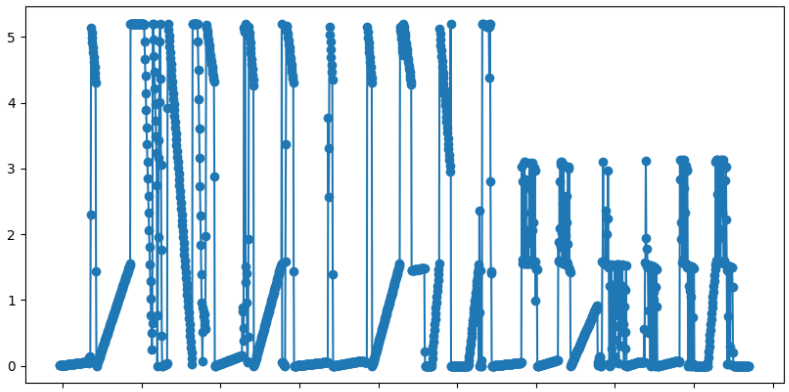
\includegraphics[width=0.5\linewidth]{figures/perfil-potencia.png}
  \caption{Modulación del perfil de potencia de una batería}
  \label{fig:perfil-potencia}
\end{figure}

Con esto, las mayores ventajas de las baterías son su capacidad de rápida conmutación o variación de su perfil de potencia y el mínimo de técnico nulo, conn el que la batería puede mantenerse inactiva sin perder capacidad de conmutación.

Para transformar la posición de mercado de energía a potencia es necesario conocer el periodo o granularidad del mercado y realizar la transformación a través de la simple ecuación~\ref{eq:energia-a-potencia}. Las limitaciones de potencia ya se han tenido en cuenta en las etapas anteriores.

\begin{equation}
  \label{eq:energia-a-potencia}
  P_{t} = E_{t} \cdot \frac{1}{\Delta t \cdot \frac{\SI{1}{\hour}}{\SI{60}{\minute}}}
\end{equation}

donde:

\begin{itemize}

  \item \( P_{t} \) es el perfil de potencia a mantener durante un periodo para ciclar una cantidad de energía en \si{\mega\watt},

  \item \( E_{t} \) es la energía a ciclar en un periodo en \si{{\mega\watt\hour}},

  \item \( \Delta t \) es la granularidad mínima de los mercados analizados en \si{\minute}.

\end{itemize}

Aún habiendo convertido las unidades, se continua teniendo un problema, explicado por el ciclado de la batería a nivel físico. El ciclado de la batería, en su formato más reductivo, está controlado por dos señales correspondientes a las fuentes de carga y descarga por el \gls{bms}, como se observa en la figura~\ref{fig:carga-descarga}. Cuando una de las señales esta activa el circuito de carga se abre, cuando la otra está activa es el de descarga el que se activa y cuando no está activa ninguna no hay flujo energético\footnote{Existen otros tipos de \gls{bms} en donde los puertos de carga y descarga son comunes, pero la restricción del control de la carga y descarga se sigue aplicando de igual manera por razones físicas para manejar la batería de ion-litio en sí, que solo observa la conexión de energía de entrada o de salida, al fin y al cabo}.

\begin{figure}
  \centering
  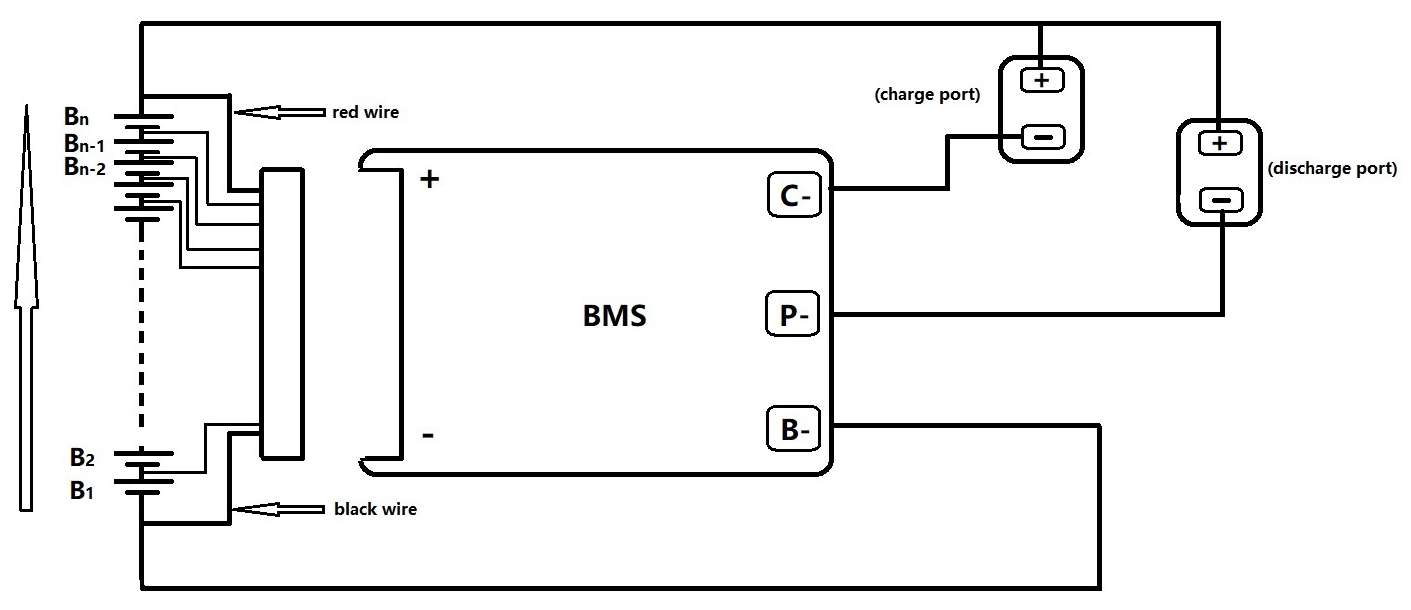
\includegraphics[width=0.5\linewidth]{figures/carga-descarga.png}
  \caption{Diagrama de un sistema de control de baterías con señales de carga y descarga independientes~\cite{sunkko2025two}}
  \label{fig:carga-descarga}
\end{figure}

¿Qué sucede entonces cuando las dos señales se activan a la vez? La activación simultanea resulta en un bloqueo mutuo donde ocurre un cortocircuito, el cual podría causar daños físicos internos a las celdas de la batería (en la practica el \gls{bms} lo impide), por esta razón la misión del sistema de control de baterías es evitar esta situación. Para ello, limita las consignas a una única señal en donde los valores positivos indican carga, los negativos descarga y cero la inactividad.

Por ejemplo, una situación en la que una carga y descarga simultanea podría suceder, de no ser por las limitaciones físicas de las baterías, es cuando existe recurso de generación limitado por restricciones técnicas para un periodo beneficioso de venta, en donde la batería querría tomarlo y venderlo directamente en el mismo periodo. Visualizado en la tabla~\ref{tab:carga-descarga-simultanea}.

\begin{table}[ht]
  \centering
  \begin{tabular}{|l|S[table-format=4.1]|S[table-format=4.1]|S[table-format=4.1]|S[table-format=4.2]|}
    \hline
    Periodo & {Batería [\si{\mega\watt}]} & {Generación [\si{\mega\watt}]} & {Instalación [\si{\mega\watt}]}  & {Precio [\si{\mega\watt}]}\\
    \hline
    H20Q1   & 5.5                       & 32.5                         & 32.5                           & -5.00\\
    H20Q2   & 5.5                       & 32.5                         & 32.5                           & 20.00\\
    H20Q3   & 0.0                       &  0.0                         &  0.0                           & 53.86\\
    H20Q4   & 0.0                       &  0.0                         &  0.0                           & 89.64\\
    H21Q1   & 5.5                       &  0.0                         & 32.5                           & 37.24\\
    H21Q2   & 5.5                       &  0.0                         & 32.5                           & 69.00\\
    H21Q3   & 5.5                       &  0.0                         & 32.5                           & 85.42\\
    H21Q4   & 5.5                       &  0.0                         & 32.5                           & 93.80\\
    H22Q1   & 5.5                       &  0.0                         & 32.5                           & 71.00\\
    H22Q2   & 5.5                       & 32.5                         & 32.5                           & 69.00\\
    H22Q3   & 5.5                       & 32.5                         & 32.5                           & 69.00\\
    H22Q4   & 5.5                       & 32.5                         & 32.5                           & 73.00\\
    \hline
  \end{tabular}
  \caption{Restricciones técnicas en donde, desde el periodo H21Q1 al H22Q1, la exportación de la generación está limitada mientras que la batería es capaz de exportar libremente, pudiendo causar conflictos entre la carga de aprovechamiento de la generación y la descarga de la venta en precios altos}
  \label{tab:carga-descarga-simultanea}
\end{table}

Para adecuarse a dichas limitaciones físicas, se combinan las señales de carga con signo positivo y descarga con signo negativo obtenidas de la optimización y posteriormente convertidas en potencia \( P = P_{d} - P_{c} \). También se añade otra capa de prevención de desactivando previamente los periodos con carga y descarga simultanea, lo cual ciertamente puede causar desvíos en el programa, pero estos serias fácilmente solucionados en optimizaciones posteriores y nunca deberían ocurrir\footnote{Los indicadores de carga y descarga simultanea introducidos en la sección~\ref{makereference5.1.2} ya lo tienen en cuenta, pero se realiza un esfuerzo para separar las responsabilidades de los diferentes roles}, de todos modos.

Con las posiciones transformadas en potencia, solo se toman en cuenta los cambios en el perfil de potencia, ilustrados en la figura~\ref{fig:diferencia-perfil-potencia}, y se anota el tiempo de inicio de cada cambio.

% TODO
\begin{figure}
  \centering
  % \includegraphics[width=0.5\linewidth]{figures/diferencia-perfil-potencia.png}
  \caption{Diferencias correspondientes al perfil de potencia final}
  \label{fig:diferencia-perfil-potencia}
\end{figure}

Por último, el envió de las consignas se realiza a través de la señal o punto ofrecido por el \gls{bms} configurado en el \gls{pis}, llamado \texttt{Programa} y explicado en el apartado de infraestructura~\ref{makereference3.2}. Se hace uso del mismo flujo descrito en la sección~\ref{makereference3.5} pero, en vez de leer señales, se escriben en los tiempos correspondientes en el historiador.

Cuando llegue el momento de cambio en el perfil de potencia de la batería y la señal del programa esté escrita en el historiado, este automáticamente enviará de vuelta un mensaje IEC 60870-5-104 a la estación marcando el nuevo perfil de potencia y la batería responderá correspondientemente.

Con esto, uno de los aspectos más cruciales no resulta ser precisamente la consignación de un nuevo perfil de potencia de carga o descarga, sino la vuelta al mínimo técnico. Es decir, es una absoluta necesidad hacer que la batería vuelva a un perfil de potencia nulo cuando se haya terminado la carga o descarga, de tal forma que no continúe ciclándose.

Interesantemente, durante el despliegue del sistema en una de las instalaciones, no se llegó a consignar correctamente la vuelta al mínimo técnico de la batería debido a un fallo lógico, por lo que esta continuó cargándose más allá del límite máximo del \( \mathrm{SoC}_{\text{max}} \) establecido y, al llegar al límite de almacenamiento, hizo saltar la alarma del \gls{bms}. El problema desplomó la disponibilidad de la batería y llegó a causar perdidas monetarias hasta rápidamente conseguir arreglarlo.

Dicha situación subraya la importancia de disponer de herramientas de observabilidad y control manual del sistema, como la descrita en la próxima sección~\ref{makereference6.2}.

\subsection{Emisión de ofertas}
\label{makereference6.1.2}

Para emitir la oferta al mercado, es necesario calcular el precio al que ofertar la posición de la batería. Para ello se emplea un algoritmo de desarrollo propio que permite agrupar las ofertas por ciclos.

En un primer momento, precisamente a los inicios de desarrollo de la emisión de la oferta, el precio de oferta se correspondía directamente al precio de mercado, como en la ecuación~\ref{eq:emisión-directa}.

\begin{equation}
  \label{eq:emisión-directa}
\end{equation}

Dicho comportamiento dispone de un fallo inaceptable en el funcionamiento del ciclado de la batería. Como el mercado eléctrico es marginalista, si existe un desvío del precio de casación a la dirección opuesta de la oferta en comparación a la predicción de precio empleada durante la operación, la oferta nunca tendrá la capacidad de casar en el mercado, resultando en un desvío de programa que, muy probablemente no podrá ser recuperado por la misma razón.

Un sencillo arreglo al previo comportamiento, empleado como evolución de la lógica de emisión de ofertas del sistema, es incluir una tolerancia de oferta en el calculo del precio. La tolerancia aumenta o disminuye el precio de oferta en la dirección opuesta al beneficio en la compra o venta, buscando la casación en el mercado, ecuación~\ref{eq:emisión-tolerancia}. Este comportamiento funciona ya que permite cubrirse ante pequeños desvíos de precio y sigue sin afectar a la disminución del beneficio si el desvío de precio es favorable. El nuevo problema, en cambio, es doble.

\begin{equation}
  \label{eq:emisión-tolerancia}
\end{equation}

Primero, el uso de una tolerancia absoluta implica que el sistema solo puede defenderse ante desvíos de precio menores pero, cuando mayor es el precio de mercado, mayores suelen ser los desvíos de precio\footnote{Si la predicción del precio de mercado supera los 100 euros megavatio hora (\textit{€/MWh}), es más probable que el precio de casación termine en un rango de 80 a 120 euros megavatio hora (\textit{€/MWh}) aproximadamente, con un desvío de precio de 20 euros megavatio hora (\textit{€/MWh}). Si la predicción es de 0 euros megavatio hora (\textit{€/MWh}), lo normal es que fluctúe en un rango de -5 a 5 euros megavatio hora (\textit{€/MWh}) o menos, un desvío de precio de 5 euros megavatio hora (\textit{€/MWh}), mucho menor}. Es complicado, por no decir imposible y poco intuitivo, seleccionar dinámicamente entre una tolerancia absoluta o relativa.

Segundo, si una de las ofertas no casa, ocurre la llamada casación parcial, en donde la batería mantiene un ciclo incompleto. Si el mercado acepta solo algunos de los periodos el estado de carga resultante puede no permitir completar el ciclo previsto o cumplir con compromisos posteriores.

Para evitar estos problemas, el sistema finalmente hace uso del algoritmo de emisión de oferta por semiciclo de carga propuesto.

Lo que se busca es agrupar los semiciclos de carga y descarga y obtener sus precios límites de compra y venta. Primeramente, se calcula la diferencia entre el estado de carga de un periodo y el anterior en la ecuación~\ref{eq:diferencia-soc}.

\begin{equation}
  \label{eq:diferencia-soc}
  \Delta \mathrm{SoC}_{t}~[\text{MWh}] = \mathrm{SoC}_{t}~[\text{MWh}] - \mathrm{SoC}_{t-1}~[\text{MWh}]
\end{equation}

Con ello, es posible calcular la dirección de cambio del estado de carga de la batería. Es decir, determinar si la batería se esta cargando, descargando o en estado estacionario, ecuación~\ref{eq:sigma-carga}. Cabe destacar que el uso del estado de carga es necesario, a diferencia del resto de resultados de la optimización, ya que este representa el \textit{source of truth} del sistema.

\begin{equation}
  \label{eq:sigma-carga}
  \sigma_{t} =
  \begin{cases}
    +1 & \text{si } \Delta\mathrm{SoC}_{t} > 0 \quad (\text{carga})\\
    -1 & \text{si } \Delta\mathrm{SoC}_{t} < 0 \quad (\text{descarga})\\
    0  & \text{si } \Delta\mathrm{SoC}_{t} = 0 \quad (\text{estado estacionario})
  \end{cases}
\end{equation}

A continuación, se calculan los llamados puntos álgidos, inferiores en este caso, en la ecuación~\ref{eq:puntos-álgidos-inf}. Los puntos álgidos representan los baremos de consideración de los semiciclos. La razón de su existencia es simple, y es que es relativamente común encontrarse con situaciones en las que la batería realiza un semiciclo sin llegar tocar estrictamente el estado de carga lleno o el máximo operacional.

Es extremadamente importante que el sistema se defienda ante situaciones de ciclado apenas completo, ya que puede que existan parámetros que no se correspondan estrictamente al comportamiento físico de la instalación, debido a diferencias en los decimales. Además, permite aumentar el control de la consideración de los ciclos desde el punto de vista de los operarios de telecontrol.

\begin{equation}
  \label{eq:puntos-álgidos-inf}
  B_{\text{inf}, t} = \mathrm{SoC}_{t}~[\text{MWh}] \le \left( \frac{\mathrm{SoC}_{\text{min}}~[\text{\%}]}{100} + \frac{\mathrm{SoC}_{\text{tol}}~[\text{\%}]}{100} \right) \cdot E_{\text{cap}}~[\text{MWh}]
\end{equation}

Como no se desea contar múltiples ciclos cuando sucedan múltiples periodos contiguos que sobrepasen un punto álgido, solo se tienen en cuenta las entradas para cada la carga y descarga. Todo ello se encuentra representado en la ecuación~\ref{eq:entrada-inf}.

\begin{equation}
  \label{eq:entrada-inf}
  B_{\text{inf}, t} =
  \begin{cases}
    0                                                & \text{si } t = 0\\
    B_{\text{inf}, t} \land \neg B_{\text{inf}, t+1} & \text{si } t > 0
  \end{cases}
\end{equation}

Se realizan los mismos cálculos para los puntos álgidos superiores en la ecuación~\ref{eq:puntos-álgidos-inf} y la ecuación~\ref{eq:entrada-sup}, teniendo en cuenta también los límites operacionales.

\begin{equation}
  \label{eq:puntos-álgidos-sup}
  B_{\text{sup}, t} = \mathrm{SoC}_{t}~[\text{MWh}] \ge \left( \min\left(\frac{\mathrm{SoC}_{\text{max}}~[\text{\%}]}{100}, \frac{A~[\text{\%}]}{100}\right) - \frac{\mathrm{SoC}_{\text{tol}}~[\text{\%}]}{100} \right) \cdot E_{\text{cap}}~[\text{MWh}]
\end{equation}

\begin{equation}
  \label{eq:entrada-sup}
  B_{\text{sup}, t} =
  \begin{cases}
    0                                                & \text{si } t = 0\\
    B_{\text{sup}, t} \land \neg B_{\text{sup}, t+1} & \text{si } t > 0
  \end{cases}
\end{equation}

A continuación, se toman juntan los puntos álgidos inferiores y superiores en la ecuación~\ref{eq:puntos-álgidos}. La razón de realizar las operaciones por separado es impedir situaciones de cargas o descargas muy rápidas, donde se sobrepasen puntos álgidos diferentes en periodos contiguos. Dentro del funcionamiento normal de las baterías, no es precisamente una situación que ocurra muy a menudo, pero es técnicamente posible que suceda.

\begin{equation}
  \label{eq:puntos-álgidos}
  B_{t} = B_{\text{inf}, t} \lor B_{\text{sup}, t}
\end{equation}

Junto a ello, se mueven los puntos un periodo en el tiempo para resolver problemas causados por el primer periodo. Se representa en la ecuación~\ref{eq:puntos-álgidos-shift}.

\begin{equation}
  \label{eq:puntos-álgidos-shift}
  B_t =
  \begin{cases}
    0       & \text{si } t = 0\\
    B_{t+1} & \text{si } t > 0
  \end{cases}
\end{equation}

Con los puntos álgidos correctamente identificados, se toma una cuenta acumulativo de los mismos. Cada número de la cuenta proporciona indirectamente un identificador unívoco sucesivo del semiciclo realizado en la ecuación~\ref{eq:conteo-ciclos}.

\begin{equation}
  \label{eq:conteo-ciclos}
  N_{\text{acc}, t} = 1 + \sum_{j=0}^{t-1} B_{j}
\end{equation}

Tan solo es dista multiplicar el conteo de los semiciclos, correspondiente con sus identificadores, con la dirección en la que operan en la ecuación~\ref{eq:conteo-ciclos-signo}. De esta forma, a cada semiciclo se le corresponde un identificador y el signo del identificador indica el tipo de ciclo, carga, descarga o estado estacionario (obtenido este último al incluir la dirección del ciclo).

\begin{equation}
  \label{eq:conteo-ciclos-signo}
  C_{t} = \sigma_{t} \cdot N_{\text{acc}, t}
\end{equation}

Finalmente, se agrupan los precios de mercado por los periodos correspondientes a cada semiciclo, ecuación~\ref{eq:agrupado-periodos}.

\begin{equation}
  \label{eq:agrupado-periodos}
  G_{i} = { P_{\text{mercado}, t} \mid C_{t} = i }
\end{equation}

Con ello, por cada grupo, se toma el precio más bajo entre los periodos de descarga y el más alto entre los de carga, añadiendo una tolerancia absoluta en la dirección opuesta al beneficio de la oferta. Esto significa que todos los periodos de un mismo semiciclo de descarga tendrán el precio menor de venta del mercado durante dicho semiciclo, mientra que exactamente lo opuesto para la carga.

\begin{equation}
  P_{\text{BESS}, i} =
  \begin{cases}
    \min(G_{i}) - T_{\text{venta}}  & \text{si } i < 0 \quad (\text{descarga})\\
    \max(G_{i}) + T_{\text{compra}} & \text{si } i > 0 \quad (\text{carga})\\
    0                               & \text{si } i = 0 \quad (\text{estado estacionario})
  \end{cases}
\end{equation}

donde:

\begin{itemize}

  \item \( \mathrm{SoC}_{t} \) es el estado de carga de la batería en el periodo \( t \), en megavatios hora (\textit{MWh}).

  \item \( \mathrm{SoC}_{t-1} \) es el estado de carga de la batería en el periodo anterior (\( t-1 \)), en megavatios hora (\textit{MWh}).

  \item \( \Delta \mathrm{SoC}_{t} \) es la diferencia del estado de carga en el periodo \( t \), en megavatios hora (\textit{MWh}).

  \item \( \sigma_{t} \) es la dirección del flujo de energía, un indicador adimensional que toma valor \(+1\) en carga, \(-1\) en descarga o \(0\) en estado estacionario.

  \item \( E_{\text{cap}} \) es la capacidad energética nominal de la batería, en megavatios hora (\textit{MWh}).

  \item \( \mathrm{SoC}_{\text{min}} \) y \( \mathrm{SoC}_{\text{max}} \) son los porcentajes mínimo y máximo del estado de carga operacional, en porcentaje (\textit{\%}).

  \item \( \mathrm{SoC}_{\text{tol}} \) es la tolerancia del estado de carga para la detección de semiciclos, en porcentaje (\textit{\%}).

  \item \( A \) es la disponibilidad de la batería, en porcentaje (\textit{\%}).

  \item \( B_{\text{inf}, t} \) y \( B_{\text{sup}, t} \) son las condiciones booleanas que indican si se ha alcanzado un punto álgido inferior o superior, respectivamente.

  \item \( B_{t} \) es la condición booleana unificada que indica si se ha completado un semiciclo en el periodo \( t \).

  \item \( N_{\text{acc}, t} \) es el contador acumulado de semiciclos, que actúa como identificador numérico del semiciclo en curso.

  \item \( C_{t} \) es el identificador del semiciclo con signo en el periodo \( t \).

  \item \( P_{\text{mercado}, t} \) es el precio del mercado eléctrico en el periodo \( t \), en euros por megavatio-hora (\textit{€/MWh}).

  \item \( G_{j} \) es el conjunto de todos los precios de mercado (\( P_{\text{mercado}, t} \)) que pertenecen a un mismo semiciclo con signo \( j \).

  \item \( P_{\text{BESS}, j} \) es el precio de oferta de referencia calculado para el semiciclo \( j \), en euros por megavatio-hora (\textit{€/MWh}).

  \item \( T_{\text{venta}} \) y \( T_{\text{compra}} \) son las tolerancias de precio para las ofertas de venta y compra, en euros por megavatio-hora (\textit{€/MWh}).

  \item \( t \) es el índice que representa el periodo de mercado.

  \item \( i \) es un índice que representa un valor único de un semiciclo, el grupo al que pertenece.

\end{itemize}

La emisión de oferta por semiciclo de carga evita aceptaciones parciales e, importantemente, refleja las restricciones intertemporales y costes de oportunidad de la batería en forma de todo o nada. Es decir, se hace uso del comportamiento más agresivo en busca de la casación en todo momento, los bloques de ofertas por semiciclo casan en todos a la vez o ninguno, siendo esta la clave.

Entendiblemente, es inevitable generar desvíos si el bloque no casa pero, inteligentemente, estos desvíos no se ven afectados por los subsecuentes movimientos en los mercados posteriores. Intentar solucionar el desvió no puede aumentarlo si se hace de esta estrategia, a diferencia de las anteriores.

Finalmente, la oferta se comunica con la herramienta externa de resolución de ofertas de la entidad energética en el formato adecuado\footnote{La emisión de ofertas del sistema soporta múltiples formatos, pero solo se muestra el usado en producción}, véase la tabla~\ref{tab:formato-oferta}. Si no es modificada, entrará automáticamente a mercado.

\begin{table}[ht]
  \centering
  \begin{tabular}{|c|c|c|c|}
    \hline
    Tipo & Descripción         & Mnemónico & Prioridad\\
    \hline
    147  & Programa de consumo & M\_PC\_AA & Baja     \\
    \hline
  \end{tabular}
  \caption{Formato de oferta de mercado}
  \label{tab:formato-oferta}
\end{table}

\section{Cuadro de mando}
\label{makereference6.2}

Aunque el sistema desarrollado sea completamente agnóstico de ningún tipo de intervención manual, significando que no es esta no es requerida para poder arbitrar en el mercado, en algunas ocasiones el sistema no es capaz de tener en cuenta todos los factores que afectan a la operación de todos los componentes involucrados en el mismo.

De hecho, uno de las situaciones más comunes encontradas a la hora de realizar el despliegue del sistema se corresponden con las indisponibilidades de la batería. Estas indiponibilidades no son causadas precisamente por las señales integradas de disponibilidad de los sistemas de almacenamiento descritas anteriormente, sino por pruebas de integración del sistema correspondientes con el funcionamiento físico de las baterías. Resulta que, al necesitar el departamento de telecontrol cerciorarse del correcto ciclado de las baterías de manera modular, es entendiblemente necesario comprobar que la consignación operativa de la sección anterior es ejecutada satisfactoriamente.

Principalmente motivado por dicho propósito y con el objetivo de facilitar las pruebas de la infraestructura, se desarrolla un cuadro de mando, como se ve en la figura~\ref{fig:cuadro-de-mando}, que permite introducir las consignas operativas manualmente, interactuando con la infraestructura operativa y el entorno de mercado, pero sorteando la modelización  estructural.

\begin{figure}
  \centering
  % 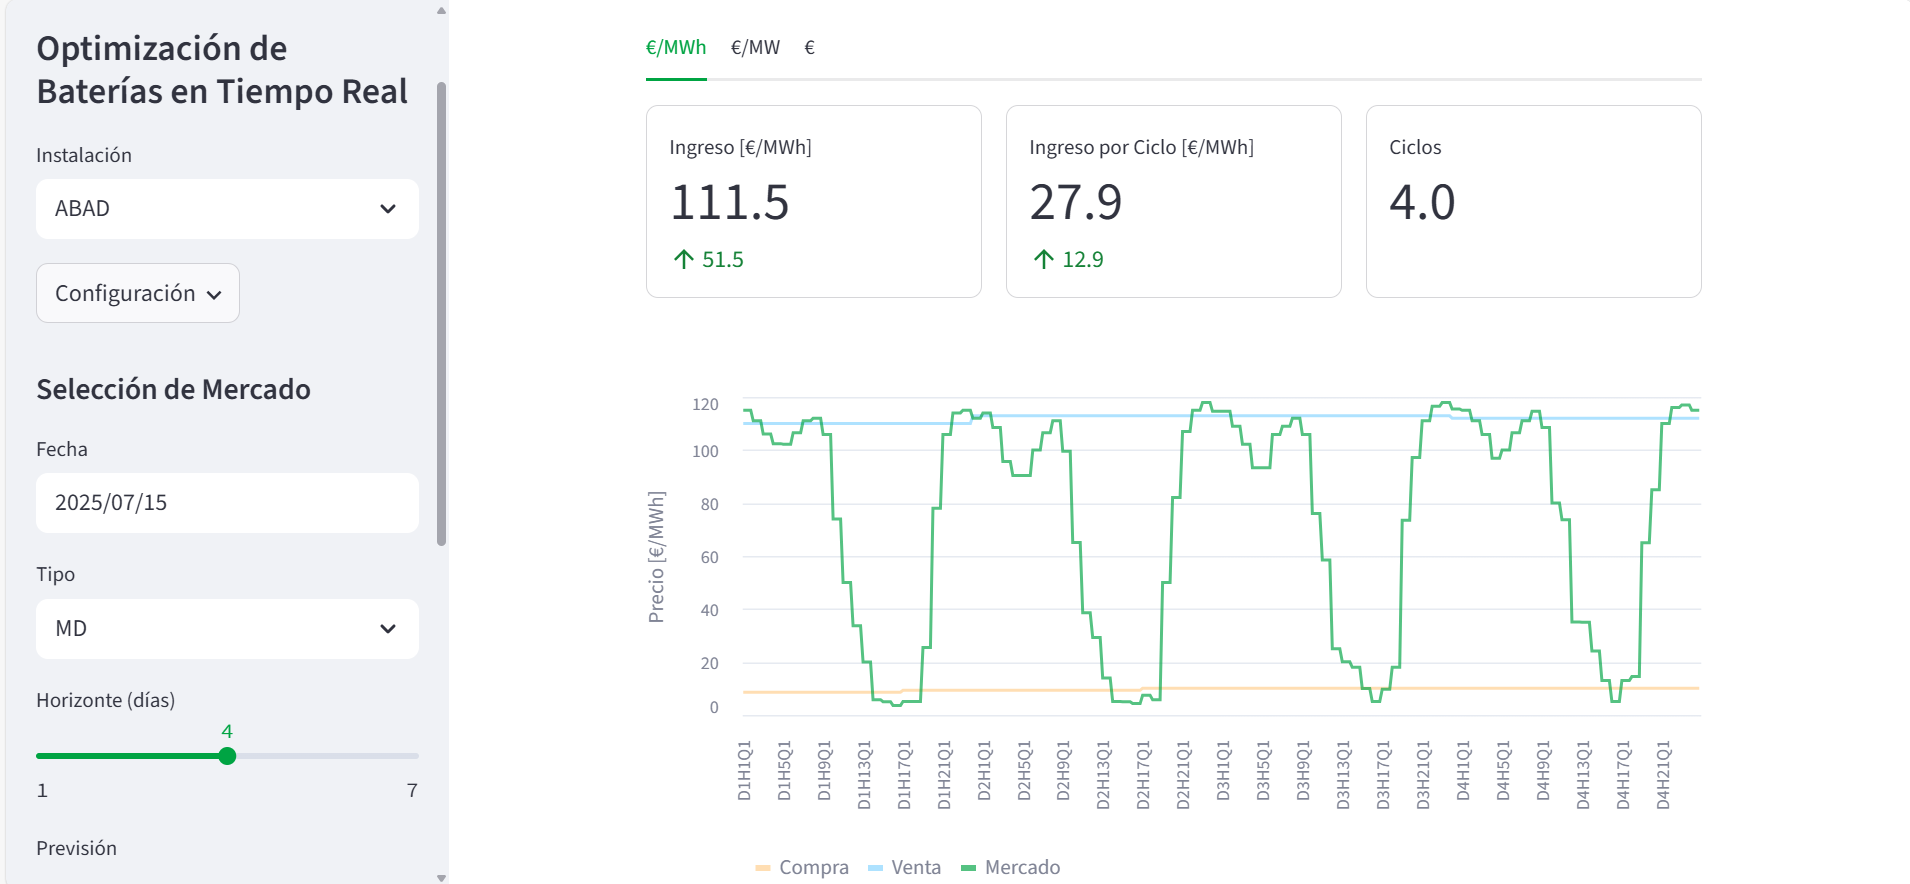
\includegraphics[width=0.5\linewidth]{figures/cuadro-de-mando.png}
  \caption{Cuadro de mando del sistema}
  \label{fig:cuadro-de-mando}
\end{figure}

Por ello, al comprobar la utilidad de la herramienta, la natural evolución de la misma resulta ser la unificación completa del control de la operación del sistema, desde la simulación de las operaciones, la consignación manual y asistida, la modificación de los parámetros operativos y la anteposición de programas.

De esta forma, el cuadro de mando del sistema es la pieza cable mediante la cual los agentes de mercado y operadores de telecontrol son capaces de interactuar al mismo tiempo con el objeto de modificar el arbitraje como les convenga. A los agentes de mercado se les da la posibilidad de cambiar las posiciones en busca de una mejor oportunidad de arbitraje impulsada por factores externos que escapan al control del sistema, y los operadores de telecontrol pueden realizar pruebas de ciclado de las baterías sin tener que interactuar con el sistema de gestión de planta y los protocolos de comunicación correspondientes. En ello reside el valor principal del desarrollo del cuadro de mandos.

Más allá del cuadro de mando del comando y control orientado a los agentes de mercado y operadores de telecontrol, el sistema también es capaz de ser configurado mediante fuentes no interactivas si es necesario, estando estas orientadas a operadores de telecontrol para la configuración de la infraestructura operativa, personal de sistemas para el entorno de mercado, y agentes de mercado para la modelización estructural.

\subsection{Experiencia de usuario}
\label{makereference6.2.1}

El cuadro de mando ha sido desarrollado en la misma tecnología principal utilizada en la mayoria de los otros componentes, Python. Esta vez, se hace uso de Streamlit, un componente para construir herramientas interactivas.

Tras pasar por un servicio de autenticación que únicamente permite el acceso a agentes de mercado y operadores de telecontrol designados, el usuario es presentado con la interfaz de operación principal.

En ella, es posible modificar la configuración operativa de cada una de las instalaciones, establecer la situación de mercado concreta a tener en cuenta y cambiar la fuente de los precios marginales explicados en la sección~\ref{makereference4.1.1}, entre otras acciones mostradas en la figura~\ref{fig:configuración-sistema}.

\begin{figure}
  \centering
  % \includegraphics[width=0.5\linewidth]{figures/configuración-sistema.png}
  \caption{Configuración del sistema a través del cuadro de mandos}
  \label{fig:configuración-sistema}
\end{figure}

Todo esto permite realizar simulaciones (por el momento) tanto a pasado y a futuro del comportamiento del sistema y de la evolución del mismo a lo largo del ciclo de vida de los mercados. Es decir, un agente de mercado es capaz de comprender fácilmente no solo lo que va a suceder el día de mañana en el mercado diario, sino también en los subsecuentes mercado intradiarios e incluso en las sesiones del mercado intradiario continuo y ver la evolución de las posiciones.

Junto a ello, se permite importar datos del mercado localmente y obviar todo el apartado~\ref{makereference3} del entorno de mercado, con el propósito de permitir el uso del cuadro de mandos en situaciones en donde no estén disponibles o se quieran modificar manualmente. Precisamente, en sinergia con la característica de exportar la información del entorno de mercado una vez obtenida, es posible realizar simulaciones más avanzadas donde todos los aspectos de entrada al sistema (incluso las señales de la infraestructura a través de la configuración de las instalaciones) sean capaces de ser modificadas.

Además, el entorno de mercado no es la única información capaz de ser exportada. Los resultados del programa óptimo de la batería, obtenido tras realizar todo el proceso, pueden ser descargados en un formato CSV con el fin de inspeccionarlos detalladamente, o incluso modificarlos (aunque resulte más intuitivo realizar cualquier modificación a través del cuadro de mandos directamente).

También se permite especificar un programa manual, en donde se asegura el seguimiento del programa mismo y la solución del modelado estructural se desactiva, y la introducción de un objetivo de estado de carga, en donde el sistema cumple con las indicaciones de estado de carga en los periodos determinados pero sigue realizando la tarea de optimización, representado en la figura~\ref{fig:soc-manual}. Crucialmente, todo el resto de validaciones siguen en funcionamiento, por lo que no es posible introducir un programa invalido de ningún modo. Se puede observar como la inclusión del objetivo de la modularización del sistema resulta más que beneficiosa antes situaciones como la descrita.

\begin{figure}
  \centering
  % 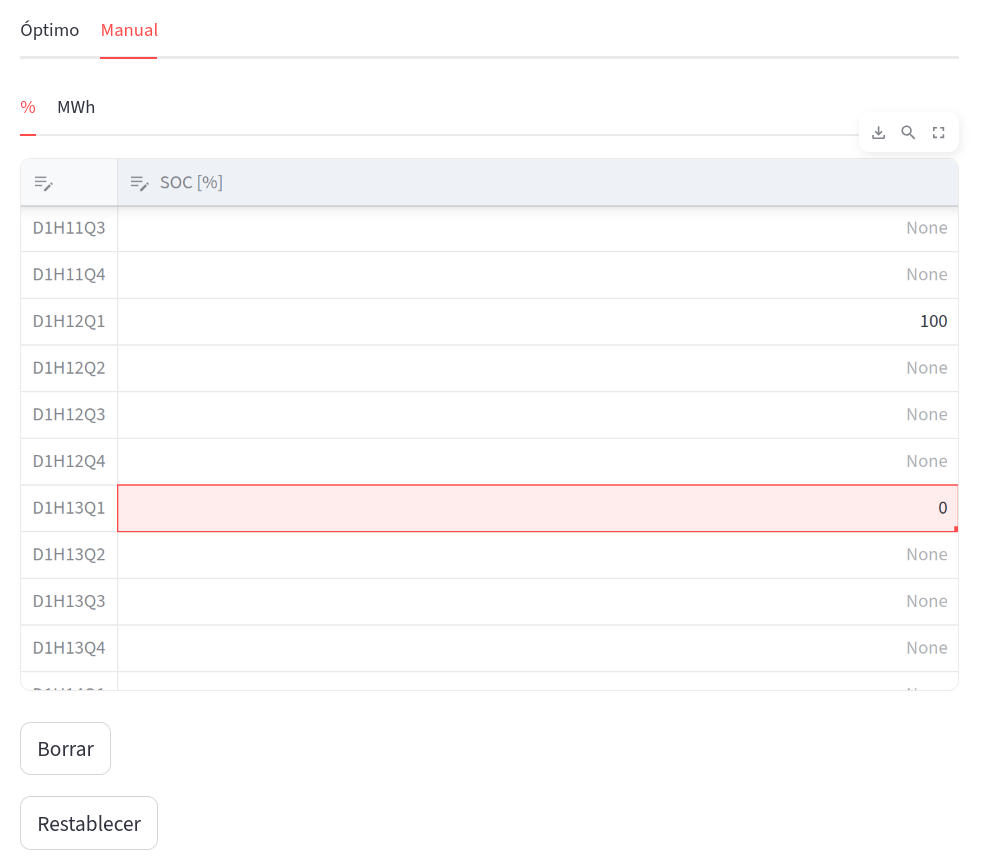
\includegraphics[width=0.5\linewidth]{figures/soc-manual.png}
  \caption{Regulación manual del estado de carga}
  \label{fig:soc-manual}
\end{figure}

En colación, es posible activar o desactivar el modo de funcionamiento manual y sustituirlo por un modo de funcionamiento automático, característica más que relevante para asegurar el cumplimiento de un programa concreto ante fallos o pruebas. Desactivado, el sistema hace caso del programa manual guardado mediante el cuadro de mandos, activado en cambio, lo sobrescribe.

Finalmente, se presentan los KPI en forma de los ingresos obtenidos por energía vendida, los ingresos totales y los ciclos realizado en diferentes unidades, dirigidos a los agentes de mercado, figura~\ref{fig:kpi-sistema}. También se muestra el perfil de generación para las instalaciones híbridas, figura~\ref{fig:perfil-generación}, junto a el programa óptimo de la batería, figura~\ref{fig:programa-óptimo}, su estado de carga a lo largo del horizonte de optimización, figura, y las limitaciones técnicas si son aplicables, figura~\ref{fig:limitaciones-técnicas}.

\begin{figure}
  \centering
  % 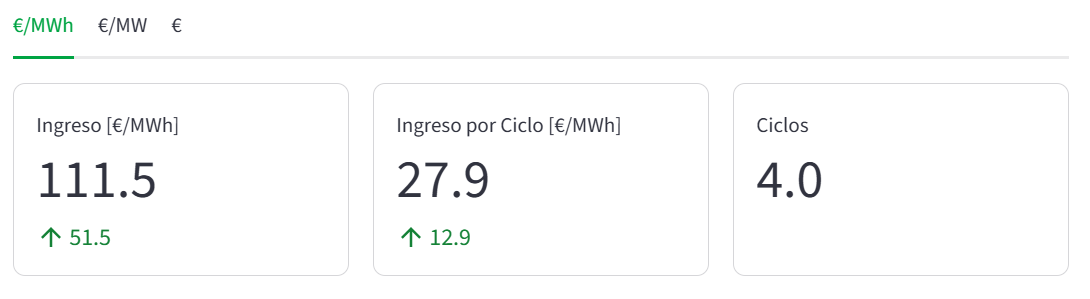
\includegraphics[width=0.5\linewidth]{figures/kpi-sistema.png}
  \caption{Métricas del sistema}
  \label{fig:kpi-sistema}
\end{figure}

\begin{figure}
  \centering
  % \includegraphics[width=0.5\linewidth]{figures/perfil-generación.png}
  \caption{Perfil de generación}
  \label{fig:perfil-generación}
\end{figure}

\begin{figure}
  \centering
  % \includegraphics[width=0.5\linewidth]{figures/programa-óptimo.png}
  \caption{Programa óptimo de la batería}
  \label{fig:programa-óptimo}
\end{figure}

\begin{figure}
  \centering
  % 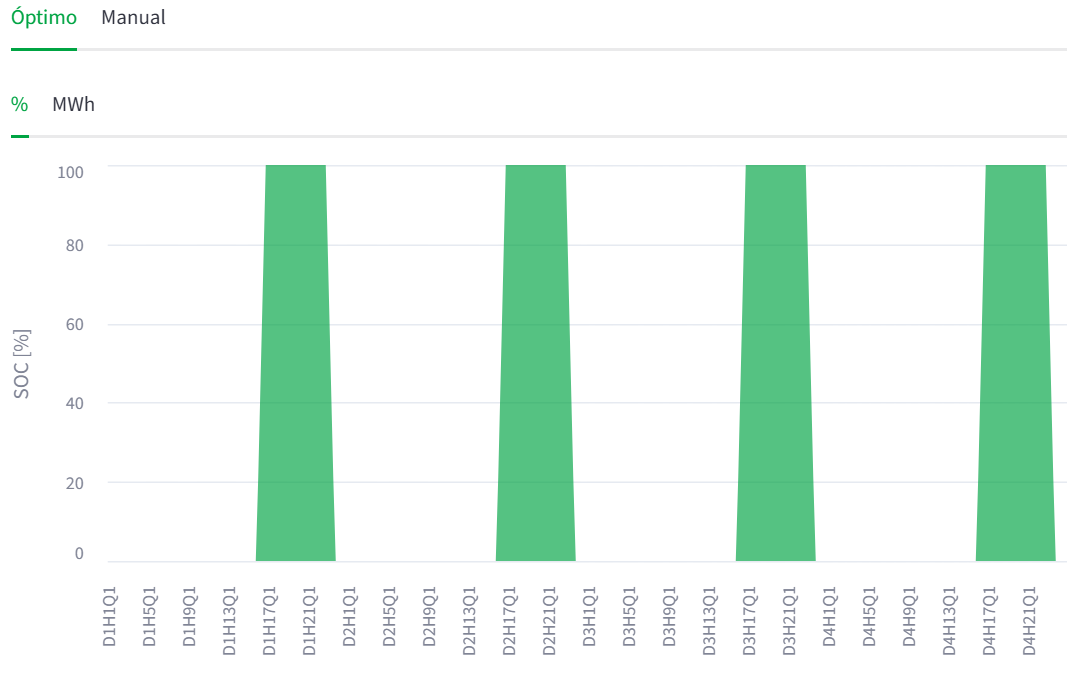
\includegraphics[width=0.5\linewidth]{figures/soc-bess.png}
  \caption{Estado de carga de la batería}
  \label{fig:soc-bess}
\end{figure}

\begin{figure}
  \centering
  % \includegraphics[width=0.5\linewidth]{figures/limitaciones-técnicas.png}
  \caption{Limitaciones técnicas de la instalación}
  \label{fig:limitaciones-técnicas}
\end{figure}

% \cleardoublepage

\chapter{Resultados experimentales}
\label{makereference7}

El sistema de optimización de baterías en el mercado eléctrico ha sido desplegado satisfactoriamente por lo menos en cuatro instalaciones, tres de topología híbrida y una de topología aislada, a lo largo de todo el país. El sistema mueve docenas de megavatios hora al día y genera millones de euros de ingreso al año.

El apartado de infraestructura operacional~\ref{makereference3} funciona continuamente obteniendo los datos de los sensores físicos de la instrumentación de campo y archivándolos en el sistema de información de planta. Los componentes del entorno de mercado~\ref{makereference4} obtienen la información del mercado, del sistema y meteorológica cada vez que cierra una sesión de mercado. La herramienta de modelización estructural~\ref{makereference5} optimiza la posición de las instalaciones con un periodo de correspondiente a la mínima diferencia entre la apertura de las sesiones de mercado. Finalmente, la consigna y control~\ref{makereference6} se comunica tanto a los activos energéticos como al mercado cada vez que se obtiene una nueva posición. El flujo se muestra en la figura~\ref{fig:flujo-procesamiento}.

\begin{figure}
  \centering
  \includegraphics[width=0.5\linewidth]{figures/flujo-procesamiento.png}
  \caption{Flujo de procesamiento de la información del sistema}
  \label{fig:flujo-procesamiento}
\end{figure}

Con esto, para obtener los resultados experimentales, ha sido necesario realizar un trabajo previo de validación con el propósito de cerciorarse de los correctos resultados de las métricas operativas, es decir, investigar la rentabilidad del sistema.

Cabe destacar que, originalmente, la entidad con la que se realizó el despliegue del sistema apenas disponía de una herramienta altamente rudimentaria con un funcionamiento incorrecto únicamente enfocada en el arbitraje de topología aislada. Esto significa que, precisamente debido a la novedad de la tecnología de almacenamiento de energía en baterías, no se ha sido capaz de realizar comparaciones con soluciones similares debido a su nula existencia dentro de la entidad misma, por lo menos.

Aún así, se ha estudiado el rendimiento obtenido al sistema, analizando su uso no solo a lo largo del periodo de despliegue, sino realizando también simulaciones con datos de mercado y señales de la batería reales. Precisamente, facilitar el llamado \textit{backtesting} resulta ser una de las razones principales para el diseño de la arquitectura del sistema modular, con el sistema de control de planta de la infraestructura operacional y la base de datos del entorno de mercado.

De esta forma, cabe destacar que la métrica principal a analizar resulta siempre ser el beneficio obtenido en euros megavatio hora. La razón del uso de la unidad recae en el hecho de que no queremos vender la mayor cantidad de energía posible en todo momento, generando grandes beneficios, sino que lo que se desea maximizar, en cambio, es el \textit{spread}. Este, siendo la diferencia entre el precio al que se ha vendido y comprado el activo correspondiente, la energía en este caso, está sujeto a la unidades del mercado, el cual opera en euros por megavatio hora.

Con ello, la configuración operativa del sistema se mantiene en un \textit{spread} mínimo objetivo de 60 euros megavatio hora (\textit{€/MWh}) y una cantidad de ciclos máximos diarios de 1. El resto de parámetros operativos varían según la instalación controlada.

\section{Rentabilidad}
\label{makereference7.1}

Primeramente, es necesario conocer la información de rentabilidad para determinar si verdaderamente merece la pena la incorporación de sistemas de almacenamiento de energía en baterías en la red eléctrica, más allá de sus beneficios operativos.

Para ello, se debe conocer el coste de capital inicial de un sistema de almacenamiento de energía en baterías estándar de ion-litio, el cual puede ascender a las cifras incorporadas en la tabla~\ref{tab:rentabilidad-bess}.

Precisamente y asumiendo la configuración más favorable descrita en las secciones posteriores como~\ref{makereference7.4}, se observa que no son solo las baterías favorables para la diversificación de la red, sino que también generan beneficios por su cuenta gracias al aprovechamiento de la energía detallado en~\ref{makereference7.3}.

Junto a ello, cabe destacar que no se han tenido en cuenta las gigantescas ayudas económicas que las entidades energéticas reciben con el propósito de promover la energía renovable. Estas ayudas, en las que se incluyen las hibridaciones renovables con sistemas de almacenamiento, inclinan la balanza a favor de las baterías.

\begin{table}[ht]
  \centering
  \begin{tabular}{|c|p{7.5cm}|c|c|}
    \hline
    Tipo & Descripción         & Mnemónico & Prioridad\\
    \hline
    147  & Programa de consumo & M\_PC\_AA & Baja     \\
    \hline
  \end{tabular}
  \caption{Rentabilidad a lo largo del tiempo de un sistema de almacenamiento en baterías}
  \label{tab:rentabilidad-bess}
\end{table}

\section{Operación manual}
\label{makereference7.2}

Pruebas empíricas en instalaciones de almacenamiento de energía en baterías en otras localizaciones en las que el sistema aún no ha sido desplegado, indican un enorme aumento en la eficiencia de la optimización.

Agentes de mercado indican tener que realizar sesiones de dos horas diarias con el único propósito de introducir las posiciones de mercado manualmente y comunicárselas a los operadores de telecomunicaciones para mandar las consignas\footnote{Aunque estas instalaciones no cuenten con el flujo desarrollado del sistema en el que las señales son comunicadas con el sistema de información de planta, existe un flujo alternativo a través de SCADA para operaciones manuales, como ya se ha descrito anteriormente}. Este trabajo de consignación manual es extremadamente propenso ha errores y completamente, o difícilmente, incapaz de aprovechar la temporalidad del proceso de optimización debido a la cantidad de combinaciones exponenciales de las posiciones de mercado cuanto más aumenta el horizonte de optimización. Situación similar a la dificultad del calculo manual del mejor movimiento en ajedrez.

La comparativa entre los resultados manuales contra el proceso del sistema desarrollado favorecen el uso de un sistema automatizado que no solo mejore de forma directa las ganancias generadas, sino que tenga en cuenta el entorno al completo y modifique su comportamiento según el mismo.

Sin disponer del sistema desarrollado, la estrategia de arbitraje más extendida entre los operadores de mercado que desvían dictar la posición de la batería se trata de la compra y venta directa de energía en los periodos valle y pico, respectivamente. Debido a la alta complejidad del arbitraje en los mercados intradiarios, los agentes de mercado únicamente definen la posición para el mercado diario de mayor liquidez.

Como se puede observar en la figura~\ref{fig:manual-vs-auto}, los dos principales problemas de la estrategia manual son el nulo aprovechamiento de los recursos híbridos de generación en las instalaciones que lo soportan, y la generación de desvíos ante falta de casaciones en el mercado diario que resultan en un perdida monetaria comparativamente significativa.

\begin{figure}
  \centering
  \includegraphics[width=0.5\linewidth]{figures/manual-vs-auto.png}
  \caption{Comparación del arbitraje entre la estrategia manual y la empleada por el sistema}
  \label{fig:manual-vs-auto}
\end{figure}

\section{Configuración topológica}
\label{makereference7.3}

Además, se han realizado análisis comparativos entre el rendimiento generado por cada una de las topologías, tanto aislada como híbrida, para determinar el aumento de beneficio que sistemas de optimización de baterías en el mercado eléctrico pueden aportar dependiendo de la configuración de la red.

Se observan las diferencias de beneficio comparativos de la figura~\ref{fig:aislado-vs-híbrido} a favor de las topologías híbridas (en su configuración más permisiva), siendo capaces de enrutar los flujos de carga desde diferentes fuentes. De esta forma, es entendible la tendencia de la industria de aumentar el número de instalaciones de colocación híbridas renovables y de almacenamiento simultáneamente.

La razón de la menor rentabilidad de la topología aislada viene dada porque su contraparte híbrida es capaz de cargar la batería en muchas ocasiones por precios nulos, mientras que la aislada siempre tiene que pagar por pasar por la red.

\begin{figure}
  \centering
  \includegraphics[width=0.5\linewidth]{figures/aislado-vs-híbrido.png}
  \caption{Resultados de arbitraje de las configuraciones topológicas de la infraestructura aislada e híbrida}
  \label{fig:aislado-vs-híbrido}
\end{figure}

\section{Topología híbrida}
\label{makereference7.4}

Una vez comprobada la mejora del uso de instalaciones de topología híbrida, resulta interesante desglosar su operación en los tres modos de operación principales observados en la practica, el híbrido flexible, el híbrido con prioridad de carga renovable y el híbrido con carga aislada de la red.

Aunque las tres configuraciones híbridas sean capaces de aprovechar y rentabilizar la energía generada, es interesante comprobar cual de ellas es capaz de generar la mayor rentabilidad, con el propósito de priorizar su instalación.

\begin{figure}
  \centering
  \includegraphics[width=0.5\linewidth]{figures/híbrido-vs-híbrido.png}
  \caption{Comparativa del rendimiento de cada topología híbrida}
  \label{fig:híbrido-vs-híbrido}
\end{figure}

En vista de los resultados obtenidos, de la figura  la configuración híbrida flexible es la que mayor rentabilidad genera, ya que es capaz de cargar tanto de la red como de la generación energética. Una de las claves de su mejora de rendimiento resultan los precios de mercado negativos. Estos, muy comunes en periodos de baja demanda, permiten obtener beneficio por comprar o cargar energía con el propósito de mantener la estabilidad de la red.

La configuración híbrida con prioridad de carga de generación, en cambio, no permite el aprovechamiento de los precios negativos ya que, irónicamente, debe priorizar la carga híbrida precisamente en los periodos de mayor generación, los cuales se corresponden con los de menor precio.

Por otro lado, la híbrida con carga aislada de la red es directamente incapaz de cargar de la red. Aunque con ella se asegure un \textit{lower bound} nulo del precio de compra, no se es capaz de aprovechar la generación al máximo debido a las restricciones de solamente poder cargar parte de la generación.

El integrador del sistema es capaz de modificar el funcionamiento físico \textit{on-site} de las instalaciones híbridas, incorporando el comportamiento flexible, para mejorar el rendimiento. Precisamente, tras el despliegue y obtención de resultados del sistema, la configuración topológica de una de las instalaciones se encuentra en proceso de modificación de híbrida con prioridad de carga renovable a híbrida flexible tras proponer el cambio.

\section{Arbitraje colaborativo}
\label{makereference7.5}

Finalmente, aunque la operación automática del sistema sea superior al control manual, eso no significa que los agentes de mercado no deban modificar su operación si piensan que es necesario para aumentar el beneficio.

Los agentes de mercado que operan el cuadro de mandos del sistema son capaces de detectar patrones externos que escapan al sistema. Uno de los fenómenos correspondientes más claro resulta ser la influencia de la temporalidad.

La temporalidad se aprecia en los precios del mercado, variando drásticamente según la demanda energética. En épocas calurosas y frías el precio aumenta, al igual que lo hace durante la semana, a diferencia del fin de semana. Con esto, es posible estudiar dicha temporalidad del mercado para atinar el ratio de ciclado de la batería: aumentarlo en las épocas más favorables y disminuirlo en las menos.

\begin{figure}
  \centering
  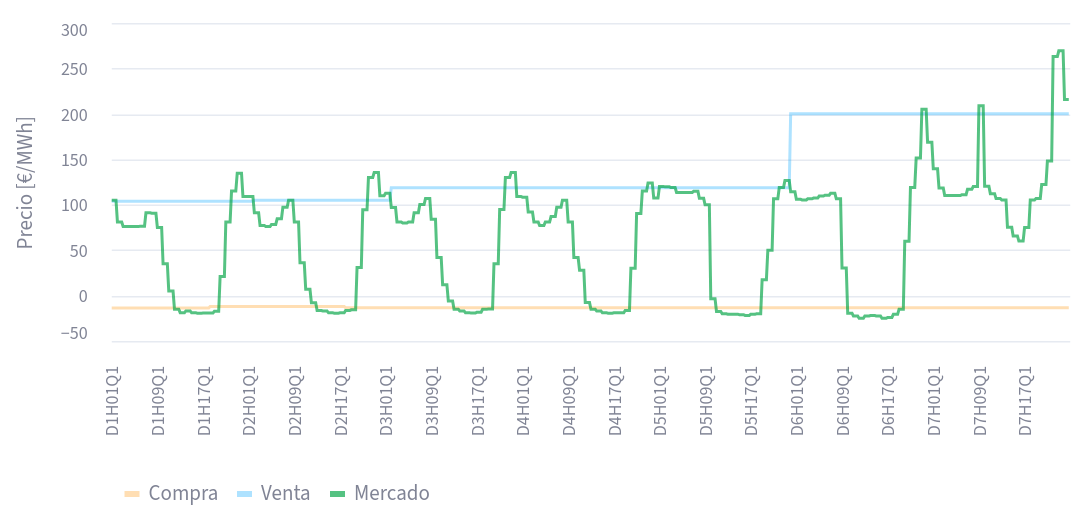
\includegraphics[width=0.5\linewidth]{figures/temporalidad-mercado.png}
  \caption{Variación del precio de mercado según el día de la semana}
  \label{fig:temporalidad-mercado}
\end{figure}

La figura~\ref{fig:temporalidad-mercado}, que representa el ciclado energético ilimitado de una batería en diferentes condiciones de mercado a lo largo de la semana, muestra la variación de los momentos oportunos de arbitraje. Lamentablemente, el ciclado de los sistemas de almacenamiento de energía debe mantenerse limitado para mantener un ritmo predecible.

Un agente de mercado operando el cuadro de mandos del sistema, en cambio, puede conocer la temporalidad del mercado eléctrico y aprovechar los altibajos para indicarle al sistema un ritmo más alto o bajo del ciclado de las baterías.

Este modo de operación se conoce como arbitraje colaborativo y es recomendable para ajustar el comportamiento del sistema en busca del mayor beneficio, siendo en consecuencia el adoptado por la entidad de mercado.

\cleardoublepage%

\chapter{Conclusiones y trabajo futuro}%
\label{makereference8}

\section{Conclusiones}%
\label{makereference8.1}

En conclusión, se ha diseñado, desarrollado, desplegado y validado satisfactoriamente un sistema de optimización de baterías a lo largo de múltiples instalaciones vinculadas a la entidad energética pertinente en la península, el cual mueve docenas de megavatios hora al día y genera millones de euros de ingresos esperados al año mediante el ciclado de \glspl{bess}, satisfaciendo así el objetivo principal propuesto. El flujo de información del sistema se representa en la figura~\ref{fig:arquitectura-control}.

\begin{figure}
  \centering
  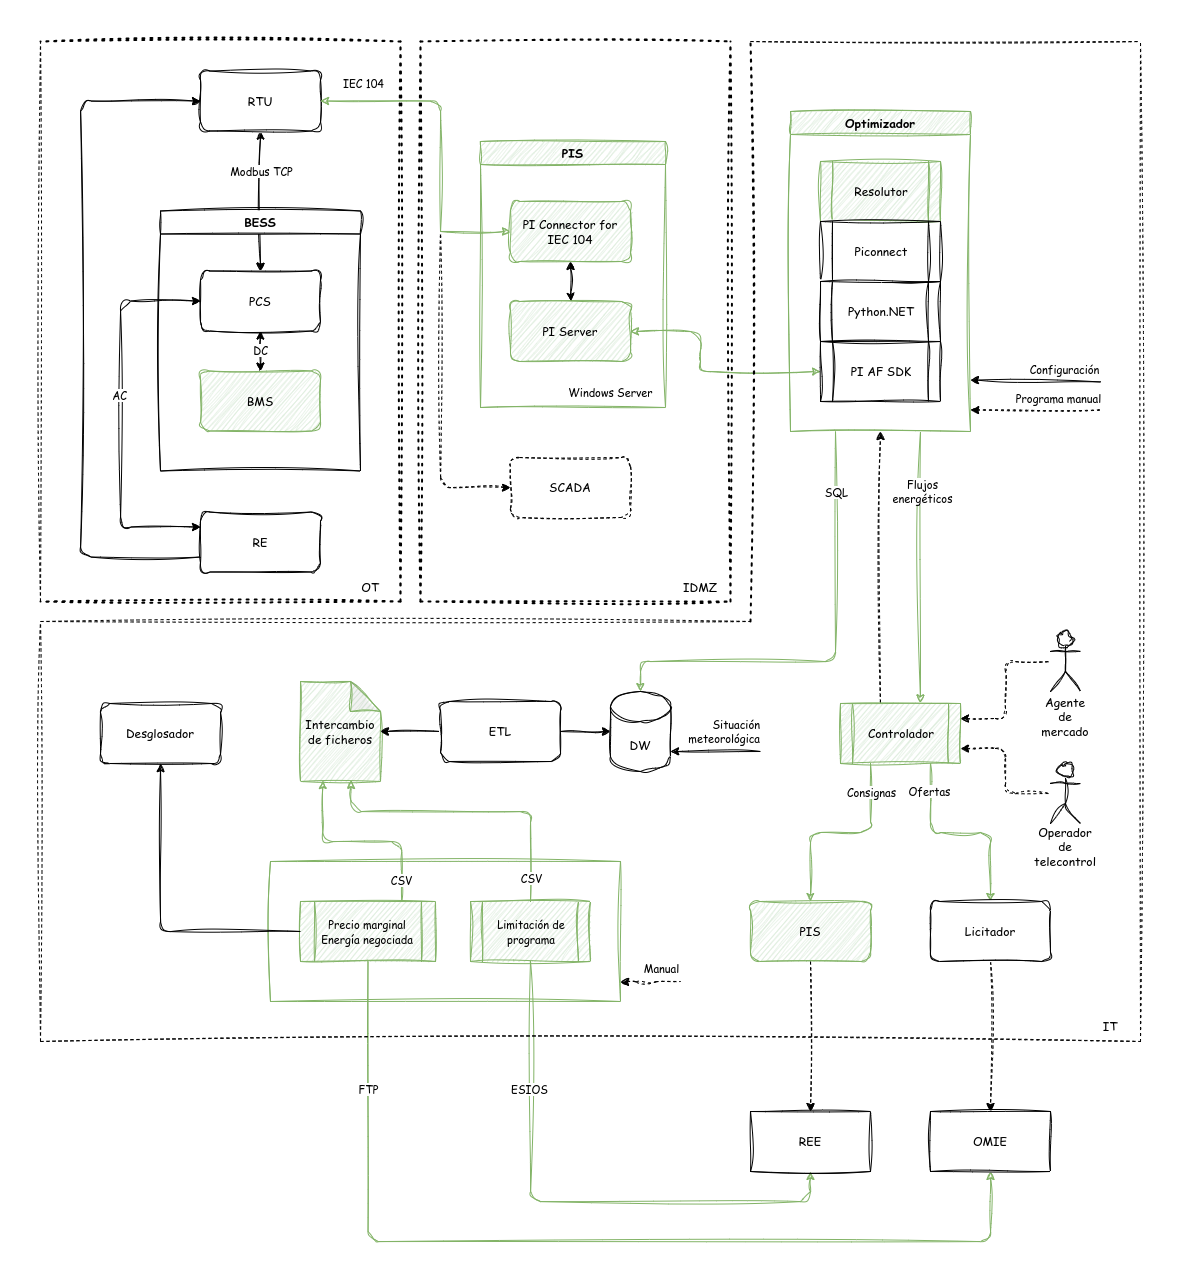
\includegraphics[width=0.9\linewidth]{figures/arquitectura.png}
  \caption[Arquitectura del sistema.]{Arquitectura del flujo de información del sistema, diferenciando los elementos pertinentes al proyecto. En términos generales, los datos de las señales de los activos son obtenidos a través de la comunicación del \gls{pis} con la red operativa, mientras que la información de mercado es extraída de las instituciones regualtorias por tareas temporizadas y depositada en ficheros a insertar en el \gls{dw}. El optimizador consulta las dos fuentes según la session de mercado y calcula los flujos de energía óptimos a realizar por los activos energéticos. Con ellos, el controlador los transforma en consignas mandadas de vuelta al \gls{pis} y ofertas a licitar. A su vez, los agentes de mercado y operadores de telecontrol son capaces de interactuar con el sistema a través del cuadro de mandos, informando al optimizador de las operaciones a realizar.}%
  \label{fig:arquitectura}
\end{figure}

A su vez, desde la perspectiva del cumplimiento de los objetivos secundarios, se ha buscado de la maximización de la rentabilidad mediante la optimización de las posiciones del mercado, junto con la consideración del desgaste de las baterías, ciclándolas de forma estable y controlada a través de la lógica de negocio de la modelización. Además, se han cumplido con los requisitos regulatorios, principalmente definidos por el operador del sistema en forma de límites técnicos, evitando así posibles penalizaciones económicas. Se ha garantizado la seguridad de la operación desplegando parte de la integración con la infraestructura física en una \gls{idmz}, evitando la exposición de la información de los activos energéticos a redes no autorizadas. También, el diseño mantiene una arquitectura generalizada, siendo capaz de operar en múltiples instalaciones sin modificación alguna de la lógica del sistema. Se han dado facilidades a los agentes de mercado y operadores de telecontrol para la monitorización del sistema y se ha tenido en cuenta la respuesta automática ante fallos, como la falta de disponibilidad. Finalmente, se ha efectuado un análisis de viabilidad económica donde se muestran resultados medibles.

Por otro lado, según el punto de vista de la arquitectura, después de analizar las configuraciones topológicas con las que trabaja el sistema, se ha unificado e implantado la nueva infraestructura operacional para tanto la adquisición de datos de los \glspl{bess} como el control de la carga y descarga de la misma, con el resto de componentes ya existentes de la red. Concretamente, se ha hecho uso de protocolos de comunicación industriales para intercambiar información con los activos energéticos e introducir la integración de las baterías con el \gls{pis}, que realiza la labor de historiador guardando los estados de las señales físicas a lo largo del tiempo para su posterior consulta. Con ello, se ha configurado la política de obtención de datos mediante mecanismos espontáneos y de \gls{gi} y se ha facilitado su lectura. De esta forma, se dibuja una paralela con las conocidas fases de un proyecto de \gls{iiot}, sensorización, procesamiento, gestión y actuación.

Junto a esto, se ha obtenido la información del entorno de mercado a través de las interfaces proporcionadas por las instituciones oficiales correspondientes, el \gls{mo} y el \gls{tso}. La información se ha procesado y transformado en el formato adecuado para su almacenamiento masivo en el \gls{dw}, la cual ha tenido que ser consultada eficientemente. Para ello, se ha hecho uso de procesos periódicos temporizados según los programas de mercado.

Más allá, se ha realizado un trabajo de modelización estructural de la situación física de las instalaciones, con el propósito de determinar la solución optima al problema de ciclado de energía de las instalaciones. Mediante un lenguaje de modelado abstracto, se han definido los comportamientos físicos de todos los tipos de instalaciones, desde las menos complejas, como las aisladas, a las más complejas, como las híbridas. Precisamente, se ha incorporado en el modela la lógica de la totalidad de los activos energéticos, tanto de almacenamiento como de generación.

Por último, se ha definido apropiadamente el comando y control del sistema, en forma de consignas de selección del perfil de potencia de las baterías y la vuelta al mínimo técnico de las mismas, junto con el calculo de los precios de oferta de mercado de las posiciones de compra y venta, mediante un algoritmo de oferta por semiciclo de carga. Además, para facilitar la supervisión a los agentes de mercado y operadores de telecontrol, se ha desarrollado un cuadro de mando a través del cual monitorizar el comportamiento automático del sistema y tomar el control manual si es necesario.

De esta forma, se ha habilitado el arbitraje de energía en el mercado en las instalaciones controladas. De no ser por el sistema desarrollado, al no existir ninguna otra solución alternativa desplegada en la península en la actualidad, las instalaciones a controlar registradas en el mercado tendrían que perder las oportunidades de arbitraje correspondientes o ser comandadas manualmente por los operarios de telecontrol, situación absolutamente inadmisible debido a la complejidad de la operación.

Cabe destacar que tanto los \glspl{bess} como, por lo tanto, los sistemas de optimización de baterías en el mercado eléctrico, se encuentran todavía en su infancia, por lo menos en el territorio europeo. Precisamente, según un estudio sobre el uso de las tecnologías de almacenamiento~\cite{hu2022potential}, ``el principal sistema de almacenamiento de energía en Europa sigue siendo el bombeo hidroeléctrico''. Esto significa que, viendo como el panorama de las tecnologías eléctricas pone su foco cada vez más en estas tecnologías de almacenamiento, es probable que salgan al mercado sistemas más sofisticados de control. Aunque, actualmente, las instalaciones con \glspl{bess} sean pocas en comparación al resto, las entidades energéticas buscan implantarlas en toda las instalaciones de generación para mejorar el aprovechamiento de la energía. Por ello, si bien el sistema implantado ha sido satisfactoriamente desplegado a lo largo de todo el país, quizás sea necesario tomar nuevas consideraciones al respecto y tener en cuenta dichas alternativas cuando la energía ciclada diariamente iguale o supere las cantidades de las de otros activos energéticos ampliamente asentados. El código disponible no confidencial censurado está disponible en GitHub\footnote{\url{https://github.com/josugoar/optibat} (unlicensed)}

\section{Trabajo futuro}%
\label{makereference8.2}

En cuanto al trabajo futuro, \textsc{Optibat} se encuentra limitado al arbitraje en los mercados spot: diario, intradiarios y continuo. Aún así, existen otros mercados más o menos rentables~\cite{cnmc2024balance}, como los mercados de \gls{mfrr} y \gls{afrr} que negocian disponibilidades. Resulta interesante añadir soporte a estos mercados para completar así el perfil de arbitraje de estas tecnologías de almacenamiento, ya que las baterías también son idóneas para la operación en dichos mercados debido a sus altas capacidades de conmutación.

Si bien la integración con los mercados de regulación es definitivamente la mejora más notable a realizar, también aporta beneficio refinar la modelización del desgaste de las baterías~\cite{shamarova2022review}. Mediante la incorporación de señales aún más granulares y las especificaciones del \gls{bms} (adaptando el sistema a cada batería), es posible modelizar incluso el imperceptible desgaste mismo del \gls{soc} de las baterías en reposo. Ciertamente, aunque no sea un aspecto sumamente prioritario, debido al constante ciclado de las baterías que, por naturaleza, no busca precisamente el mantenimiento en estado estacionario, el aporte sustancial toma forma del aumento de fidelidad de los procesos físicos modelados. Además, un análisis en profundidad del desgaste sufrido por la batería, más allá del consumo de los ciclos para los que está calificada por el fabricante, brinda claridad a posibles optimizaciones del beneficio obtenido bajo condiciones más adversas que las experimentadas.

Junto a ello, el trabajo futuro más realista viene dado en forma de la implantación del sistema de optimización desarrollado en el creciente número de nuevas instalaciones híbridas con activos energéticos de almacenamiento en incorporación continua a la red. Como ya se ha detallado anteriormente, los \glspl{bess}, al ser todavía una tecnología no tan ampliamente establecida, se encuentran en continuo crecimiento. De hecho, incluso durante el proceso de desarrollo se hizo disponible un nuevo sistema de almacenamiento.

Cabe destacar que se han esfuerzos para el mantenimiento y mejora del trabajo desarrollado dentro de la entidad energética pertinente, con el objetivo de garantizar la continuación de su ciclo de vida, de tal forma que su operación y despliegue prosigan bajo la supervisión de un equipo diferente.


\nocite{*}
\bibliographystyle{plainnat}
\bibliography{references}
\addcontentsline{toc}{chapter}{Bibliografía}

\appendix
\cleardoublepage

\glsaddall
\printacronyms[title=Acrónimos]


\end{document}
